% Copyright (c) 2024 by Toby Thurston. This material may be distributed only}
% subject to the terms and conditions set forth in the Open Publication License,
% v1.0 or later (the latest version is presently available at
% http://www.opencontent.org/openpub/).
 
% \loop\iftrue 
% \errmessage{This manual is copyrighted and should not be compiled as is.}
% \repeat
\documentclass[a4paper,landscape]{article}
\usepackage{luamplib}
\mplibtextextlabel{enable}
\everymplib{beginfig(0);} \everyendmplib{endfig;}
\usepackage{fontspec}
\newfontfamily{\demo}{TeX Gyre Pagella}
\DeclareTextFontCommand{\textdemo}{\demo}
\usepackage[inner=1in,textwidth=5in,textheight=6in, marginparsep=0.5in, marginparwidth=4.2in]{geometry}
\usepackage{sectsty}
\allsectionsfont{\normalfont\sffamily\bfseries}
\usepackage{graphicx}
\usepackage{mflogo}
\def\mfbook{\textsl{The \MF\kern1pt book}}
\def\texbook{\textsl{The \TeX\kern1pt book}}
\usepackage{shortvrb}\MakeShortVerb{"}
\usepackage{enumitem}
\usepackage{dwmpcode}
\title{Drawing with Metapost}
\author{Toby Thurston}
\date{March 2017 – October 2024}
\overfullrule=2pt
\def\kw#1{\begingroup\def\_{\kern.04em\vbox{\hrule width.3em height .6pt}\kern.08em}%
\ifmmode\mathop{\textbf{#1}}\else\textbf{#1}\fi\endgroup}
\def\op#1{\begingroup\def\_{\kern.04em\vbox{\hrule width.3em height .6pt}\kern.08em}%
\ifmmode\mathop{\textrm{#1}}\else\textrm{#1}\fi\endgroup}
\def\id#1{\begingroup\def\_{\kern.04em\vbox{\hrule width.3em height .6pt}\kern.08em}%
\ifmmode\mathop{\textit{#1}}\else\textit{#1}\fi\endgroup}
\def\cycle{\textrm{cycle}}
\def\vpic#1#2{\moveright5.5in\vbox to 0pt{\hsize4in\vskip#1\centerline{\includegraphics{#2}}\vss}}
\def\mpic#1#2{\vadjust{\moveright5.5in\vbox to 0pt{\hsize4in\vskip#1\centerline{\includegraphics{#2}}\vss}}}
\def\mnote#1#2{\vadjust{\moveright5.5in\vbox to 0pt{\hsize4in\vskip#1\noindent #2\par\vss}}}
\def\mwpic#1#2{\vadjust{\moveright5.5in\vbox to 0pt{\hsize4in\vskip#1\centerline{\includegraphics[width=4in]{#2}}\vss}}}
\def\mxpic#1#2#3{\vadjust{\moveright5.5in\vbox to 0pt{\hsize4in\vskip#1\centerline{\includegraphics[width=#2]{#3}}\vss}}}
\def\nb{$\vcenter{\begin{mplibcode}
for t=0 upto 3: fill unitsquare scaled 4 shifted right shifted up rotated 45 rotated 90t;
endfor currentpicture := currentpicture scaled 1/2; \end{mplibcode}}$\ }
\def\unit#1{\ifmmode\,\else\thinspace\fi\hbox{#1}}
\def\to{\mathrel{\ldotp\ldotp}}
\def\<#1>{\ensuremath{\langle\hbox{#1}\rangle}}
\usepackage{pifont}
\def\hey{\llap{{\ding{43}}\ }}
\newcommand\fleuron{\begin{mplibcode}
  -z1 = z4 = 7 dir 8; 
  y2 - y1 = y4 - y3 = 3(y4 - y1);
  z2 - z1 = z4 - z3 = whatever * dir 50;
  draw z1 .. controls z2 and z3 .. z4 
    withpen pencircle xscaled 1.2 yscaled 0.2 rotated 50;
  currentpicture := currentpicture rotated - angle z4;
\end{mplibcode}}
\newcommand\continued{\moveright 296pt\vbox to 0pt{\vskip -36pt
\begin{mplibcode}
  ahangle := 30;
  drawarrow origin {right} .. {dir 60} 42 dir 60;
  label.lft("\small \dots continued", origin);
\end{mplibcode}\vss}}
%
\begin{document}
\let\folio\thepage
\renewcommand{\thepage}{\rlap{\hbox to 5in{\hss\small\folio}}}
\pagestyle{myheadings}
\raggedbottom
% title & toc in the margin
\makeatletter
\moveright 6in\vbox to
0pt{\vskip23pt\noindent\sffamily{\Large\bfseries\@title}\par\bigskip
    \noindent\@author\ --- \@date\par
    \bigskip\noindent
    \includegraphics{archimedes.pdf}
\vss}
\makeatother
\thispagestyle{empty}
\section{Start here}

This document contains a collection of ideas and techniques for producing attractive
technical drawings with John Hobby’s \MP\ language.  I’m assuming that you already
know the basics of the language, that you have it installed as part of your up to
date \TeX\ ecosystem, and that you have established a reasonable workflow that
let’s you write a Metapost program, compile it, and include the results in your
\TeX\ document.  If not, you might like to start at the \MP\ page on CTAN, and read
some of the excellent tutorials, including "mpintro.pdf".  If you have already done
this, please read on.

These notes are partly based on the examples I have developed as answers
to questions about technical drawing on the \TeX\ Stack Exchange site.  In
accordance with their terms and conditions, I’ve only included material here that
I’ve written myself --- if you want other people’s code then visit the site;
while most answers there focus on writing \LaTeX\ documents, there are a great
many questions about drawing, and some of the answers are very illuminating.

My approach here will be to explore plain \MP, with examples grouped
into themes.  One approach to using this document would be to read it end to end.
Another would be to flick through until you see something that looks like it might
be useful and then see how it’s done.

And when I say \textit{plain} \MP\ I mean \MP\ with the default format (as defined
in the file "plain.mp") loaded and only a few simple external packages (like
"colorbrewer") occasionally.  Nearly all of the examples here are supposed to be self
contained, and any macros are defined locally so you can get to grips with what’s
going on.  \MP\ is a very subtle language, and it’s possible to do some very clever
and completely inscrutable things with it;  but here I have tried to be as clear as
possible in my examples.

\vbox to 0pt{
\vskip 1in
\noindent
\begingroup\footnotesize\blue{
Copyright \copyright\ 2024 by Toby Thurston. This material may be distributed only
subject to the terms and conditions set forth in the Open Publication License,~v1.0
or later (the latest version is presently available at
"http://www.opencontent.org/openpub/").}\endgroup\par\vss}

\newpage
\section{Some features of the syntax}

\begin{itemize}
    \item Assignment or equation:  the equation "a=3;" means “"a" is the same as "3" throughout the
        current scope”; the assignment "a:=3;" means “update the value of "a" to the value "3"
        immediately”.  The difference becomes apparent when you try to update a
        variable in the same scope.
        \mwpic{0pt}{tiling}

        This difference also lets you write linear equations
        like "a=-b;".  After this, as soon as you give  a value to "a", \MP\ immediately works
        out the value of "b".
        This is clever but has its limitations.  As the following snippet reveals:
\begin{code}
  % if you run this       you will get this in the log
  a + b = 0; show (a,b);  % >> (a,-a)
  a=42;      show (a,b);  % >> (42,-42)
  a:=43;     show (a,b);  % >> (43,-42)
\end{code}
        As soon as you assign to variable with ":=" \MP\ breaks any previously
        established equations.

    \item Variable types:

        —
        \<numeric> "a",
        \<pair> "(a,b)"

        —
        \<color> "(r,g,b)",
        \<cmykcolor> "(c,m,y,k)"
        \<transform> "(x,y,xx,xy,yx,yy)"

        —
        \<string>,
        \<path>,
        \<picture>


        If you don’t declare a variable, it’s assumed that it’s a \<numeric>.
        When you do declare a variable --- \<numeric> or otherwise — any value that it
       already had in the current scope is removed.

    \item Implicit multiplication: \MP\ inherits a rich set of rules about numerical
        expressions from \MF, and of special interest is the scalar multiplication
        operator.  Any simple number, like "42", "3.1415", or ".6931", or any simple
        fraction like "1/2" or "355/113" standing on it’s own (technically at the
        primary level) and not followed by "+" or "-" becomes a scalar
        multiplication operator that applies to the next token (which should be variable
        of some appropriate type).
        So you can write things like "3a", or even "1/2 a"
        (the space between the number and the variable name is optional). This
        lets you write very readable mathematical expressions. It’s quite
        addictive after a while.

\end{itemize}

\vskip -22pt
\moveright5.5in\vbox to 0pt{\vss\hsize 4in\noindent
The \mpl{sqrt} operator is defined at the same (top) level of precedence, so
that \mpl{sqrt2+1} is read as \mpl{(sqrt2)+1} and not \mpl{sqrt(2+1)}, but fractions
trump even that, so \mpl{sqrt 1/2 = 0.7071} is true.}

\newpage
\section{Workflow}

This document is not meant for beginners, so you won't find step by step tutorials
for something so simple as running \MP.  But since you might not find it all that
simple, and since the basic tutorials can go out of date, here are descriptions of
my own workflows that you might find helpful.  You might also think I'm being really
inefficient; if so please drop me a line and suggest an improvement.

The common features of each of these workflows are: Mac~OS, the MacVim editor to
edit \MP\ source code, and
Skim.app to view PostScript and PDF files.  I have the complete MacTeX distribution
installed; any commands mentioned below are supplied by MacTeX.

\subsection{Stand alone graphics with plain \MP}\label{sec:plain-flow}

\MP\ source files have the extension ".mp", when I open a file in MacVim that
matches "*.mp", my editor profile sets the file type to "mp" (which picks up the
highlight and indentation rules supplied with MacVim), and adds some relevant
directories to the search tree.  Finally, if the file is a new file, then the
profile loads this template:
\begin{smallcode}
prologues := 3;
outputtemplate := "%j%c.%{outputformat}";
beginfig(1);

endfig;
end.
\end{smallcode}
The first two lines are important: "prologues := 3;" makes \MP\ put the full font
details in the output so that the files are self-contained; the "outputtemplate"
line means that the output will be written to files with an extension that matches
the chosen output format, which will be "png", "svg", or more usually "eps", which
is the default (and suggests that the output is Encapsulated PostScript).

\smallskip

I then add drawing and label commands, using all the traditional facilities for
typesetting labels described in section \ref{sec:trad-labels}.  I compile the source
with "mpost". I usually do this from within MacVim using the command line ":!mpost %"
where "!" means “this is an external command” and the "%" picks up the current file
name.  Usually I need several attempts to get a diagram right, so I open Skim to preview the
output. 
\vadjust{\moveright5.4in\vbox to 0pt{\vss\hsize 4in\noindent
$$\includegraphics[width=4in]{workflow-plain.pdf}$$
Until recent (2024) versions of Mac~OS, it was possible to get Skim to view the
PostScript output directly, with automatic updates on recompile,
but the conversion from PostScript no longer works properly, so 
I now prefer to convert the EPS to PDF using "epstopdf". This 
slightly complicates the edit, compile, and preview loop.  On the other hand
the PDFs are generally more useful files to create, so it is worth the extra effort.  

I use a small Python script to automate the process: run
"mpost" with the "-recorder" option; scan the list of files to see what got
produced; check which ones are PostScript; call "esptopdf" to make each one into a
PDF file; remove each EPS file if successful.  Your mileage may vary.\par
}}

\subsection{Stand alone graphics with Lua\LaTeX}\label{sec:sa-lua-flow}

For graphics with more complicated text formatting, I prefer now to use
\texttt{lualatex} with the \texttt{luamplib} package.  \mpic{0cm}{workflow}
The work flow is a bit simpler because there are no intermediate EPS files to worry
about.  Instead of compiling with plain "mpost" I use "lualatex" with the "luamplib"
package, which calls \MP\ from within the Lua environment.  The \MP\ engine actually
used is exactly the same.  Here is
the template I use:
\begin{texcode}
\documentclass[border=5mm]{standalone}
\usepackage{luamplib}
\mplibtextextlabel{enable}
\begin{document}
\begin{mplibcode}
\end{texcode}
\vskip-12pt
\begin{smallcode}
    beginfig(1);

    endfig;
\end{smallcode}
\vskip-12pt
\begin{texcode}
\end{mplibcode}
\end{document}
\end{texcode}
As you can see, we have \MP\ source code wrapped up in a minimal \LaTeX\ document
using the \texttt{standalone} class, which automatically adjusts the page size to
fit the contents of document, so is ideal for single diagrams.  One small
disadvantage is that you can only produce a single PDF output file, so you need to have a
separate file for each picture, but the good news is that you get a much simpler and
more effective integration with \LaTeX, in particular with the font environment, but
as this only works with "lualatex" you have to use the "fontspec" package, as
explained in section \ref{sec:neo-labels}.\vadjust{\moveright5.5in\vbox to 0pt{\vss\hsize 4in\noindent
\hey\small If you like the fancier \MP\ format provided with Con\TeX t, you can use it directly with this
"luamplib" approach.  Just add this option to your preamble:
\begin{texcode}
\mplibsetformat{metafun}
\end{texcode}}}

\subsection{Integrated graphics with Lua\LaTeX}\label{sec:lua-integrated}

If you are ready to use "lualatex" for processing your entire document, then you can
directly embed your \MP\ drawings in a series of "mplibcode" environments.  Each one
produces a horizontal-mode box.  For details try "texdoc luamplib".  The only
drawback of this all-in-one approach is that you have to compile all the drawings
every time you compile the document, which might slow you down --- although on a
modern machine this is not really an issue any more.

\newpage
\section{Making and using paths}
\label{plain-shapes}

In \MP\ there are two sorts of paths: open and closed.
\mpic{-12pt}{closed-triangles}
A closed path is called a cycle, and is created with the \mpl{cycle} primitive like this:
\begin{code}
path t; t = origin -- (55,0) -- (55,34) -- cycle;
\end{code}
You can think of \mpl{cycle} as meaning ‘connect back to the start and close the path’.
Note that you have explicitly put \mpl{cycle} to make a closed path.  If you wrote 
\begin{code}[xrightmargin=-32pt]
path u; u = origin {right} .. (55,0) .. (55,34) .. {-2,-1} origin;
\end{code}
then $u$ would be an open path even though the last point is the same as the
first.  Any path that does not have \mpl{cycle} at the end is an open
path.\mpic{-12pt}{open-triangle}

You can use \mpl{draw} with either sort of path, but you can only use \mpl{fill} with a
cycle.  This concept is common to most drawing languages but it’s often hidden:  an
open path might be automatically closed for you when you try to fill it.  \MP\ takes
a more cautious approach; if you pass an open path to \mpl{fill} you will get an error
that says ‘Not a cycle’, even if the first and last points are the same like path
$u$ above.  

If you want to write a macro that deals differently with the two types
of path, then you can use \mpl{cycle} in a boolean context to test
whether a given path $p$ is closed:
\begin{code}
    if cycle p:
        % do something for closed path p
    else:
        % do something for open path p
    fi
\end{code}

\smallskip\noindent
\MP\ inherits the rich path-making syntax directly from \MF, so if you want a
general refresher, or you are not
quite sure what the five joiners do, $\longrightarrow$\marginpar{%
    \vbox to 0pt{\vss\halign{\kern .5in\mpl{#}\hfil\quad&#\hfil\cr
..&free curve\cr
...&bounded curve\cr
--&straight line\cr
---&tense line\cr
\&&splice.\cr}\vss}} or you would like to bone up on exactly what \mpl{curl} and
\mpl{tension} are for, then you are recommended to review Chapter 14 of \mfbook.  

\vfill\noindent
Most of the examples in this document use only the two simple joiners \mpl{--} and
\mpl{..} with the occasional use of a direction-specifying pair before or after a
point.

\clearpage
\subsection{Predefined closed paths}

There are several closed paths defined for you in plain \MP.
\mpic{-36pt}{closed-standards}
\begin{itemize}
    \item "unitsquare" is defined as the path
        \mpl{(0,0)--(1,0)--(1,1)--(0,1)--cycle}.  It runs counter-clockwise from the
        origin, and you can use it to draw any rectangle with appropriate
        use of \mpl{xscaled} and \mpl{yscaled}, or a parallelogram with \mpl{slanted},
        or a diamond with \mpl{rotated} --- but note that the definition means
        that is it centred on point \mpl{(1/2, 1/2)} so you might want to 
        shift it by \mpl{-(1/2,1/2)} before you transform it.

    \item "fullcircle" which you can use to draw any circle or ellipse with
        appropriate use of \mpl{xscaled} and \mpl{yscaled}.  Unlike the square, it is defined so that it is centred
        at the origin.  But beware that it has unit \textit{diameter}, so its radius
        is $0.5\unit{bp}$ long.  The path runs counter-clockwise and starts at 3
        o’clock; which means \mpl{point 0 of fullcircle = 1/2 right} is true. 

    \item "superellipse()" which creates the shape beloved of the Danish designer Piet Hein.  Unlike the
        other two, this one is defined as a function rather than a \<path> constant, so you need to call it
        like this:
\begin{code}
path s; 
s = superellipse(1/2 right, 1/2 up, 1/2 left, 1/2 down, 13/16);
\end{code}
        to create a ‘unit’ shape that matches \mpl{fullcircle} as shown above.
        The fifth parameter is the ‘superness’: the value \mpic{-132pt}{closed-superellipses}
        1 makes it look almost square; $\frac12$ gives you a diamond; a value somewhere
        between $\frac34$ and $\frac78$ looks about right.\quad$\longrightarrow$\\
        Values outside the range $(0.5,1)$ give you rather weird propeller
        shapes.

\noindent
\hey Note that, unaccountably, $\id{superellipse}()$ is defined in
        \texttt{plain.mp} with a \kw{def} rather than a \kw{vardef}.  This means you
        need to enclose it in a group before you can transform it in any way. One
        way to do this is to use parentheses; or you can assign it to a \<path>
        variable, as shown above.

\end{itemize}


\newpage\subsection{Points on the standard closed paths}

\noindent\mpic{-10pt}{closed-points}%
\textsc{Here are the three shapes} centred on the origin and labelled to show the points
along them.  \textbf{Note} that the \textit{unitsquare} shape has been shifted so that it is
centred on the origin in all of these examples.  The small red circle marks the
\textit{origin}, and the labelled red dots are the points of each path.  The
\textit{unitsquare} has four points, while the other two shapes both have eight.
The small
arrows between point~0 and point~1 of each shape indicate the direction of the path
that makes up the shape.

\vfill\noindent
If you want to highlight a segment of your shape, there’s a neat way to define it
using "subpath".  Assuming "p" is the path of your shape, then this:
\begin{code}
center p -- subpath(1,2) of p -- cycle
\end{code}
creates a useful wedge shape which looks like this in our three ‘standard’
shapes.

\vfill\noindent
Better still, you are not limited to integer points along the path of your closed shape.
So if you wanted a wedge that was exactly $1/5$ of the area of your shape, you
could try
\begin{code}
center p -- subpath(0,1/5 length p) of p -- cycle
\end{code}
Clearly this works rather better with more circular shapes.  Indeed for a circle you
can convert directly between circumference angle and points along the path.  So you
have defined path $c$ to be scaled copy of \mpl{fullcircle}, then \mpl{point 1 of c}
is $45^\circ$ round and 1~radian is \mpl{point 1.27324 of c}, (because $4/\pi \simeq
1.27324$).

\vfill\noindent
In a closed path, the point numbering in \MP\ wraps round: so in a
circle, point $n$ is the same as point $n+8$; and in general point $n$ is the same as
point $n+\kw{length} p$.  This works with negative numbers too, so we could use
\begin{code}
center p -- subpath(-1,1) of p -- cycle
\end{code}
to get wedge that extends either side of point 0.
The same idea was used to draw the arrows in the first row:
\begin{code}
drawarrow subpath(1/2, length p + 1/2) of p;
\end{code}

\newpage
\subsection{Regular polygons of a given radius}\label{polygons}

\noindent\mpic{-10pt}{closed-polygons}%
\textsc{Regular polygons} with a given radius can be defined or drawn directly with a simple inline loop:
\vadjust{\moveright -60pt \vbox to 0pt{\vskip-3pt\includegraphics{little-hexagon.pdf}\vss}}
\begin{code}
draw for i=0 upto 5: 20 dir 60i -- endfor cycle;
\end{code}
which works because \mpl{dir d} expands to \mpl{right rotated d}.  But
you might prefer to make a macro:
\begin{code}
vardef polygon(expr n, r) = 
    for i=0 upto n-1: (r, 0) rotated (360/n * i) -- endfor cycle 
enddef;
\end{code}
This produces a closed path to represent an $n$-sided polygon that fits in a circle
of radius $r$ centred at the origin and that starts at \mpl{(r, 0)}, like the
corresponding circular path, as shown in this polygonal version of the
previous segment chart.\rlap{\ $\rightarrow$}\\
If you need polygon paths that start at the top, you can just swap the
coordinates:
\begin{code}
vardef polygon(expr n, r) = 
    for i=0 upto n-1: (0, r) rotated (360/n * i) -- endfor cycle 
enddef;
\end{code}
$$\includegraphics[width=0.66\textwidth]{closed-polygon-tops.pdf}$$
\hey Note also that some extra care is required to find the centres of these shapes. The
\mpl{center} macro defined in "plain.mp" gives you the centre of the bounding box,
but this is not the same as the centre of the polygon when the number of sides is
odd.  What you need instead is the geometric center or \textit{centroid}:
\begin{code}
vardef centroid primary p = 
  origin for i=1 upto length p: + point i of p / length p endfor
enddef;
\end{code}
This should work for any closed path, not just regular polygons.  For ways to 
label the vertices neatly, as shown above, see §\ref{sec:new-dynamic}.

\newpage
\subsection{Regular polygons of a given side length}\label{polygons-given-side}
But you might want a polygon with a fixed side instead of a fixed radius. This needs
a little trigonometry, using the sine rule:\mpic{-60pt}{closed-fixed-polygon}
\smallmpexternal[firstline=7, lastline=11]{closed-fixed-polygon.mp}
\noindent
Which you can use like this to produce a nest of polygons \rightarrowfill
\smallmpexternal[firstline=12, lastline=16]{closed-fixed-polygon.mp}

\vfill
\noindent
These polygon paths are centred on $(0, 0)$ but
sometimes it is more convenient to construct a polygon on a known segment
rather than working out how to rotate and shift it into place.  
$$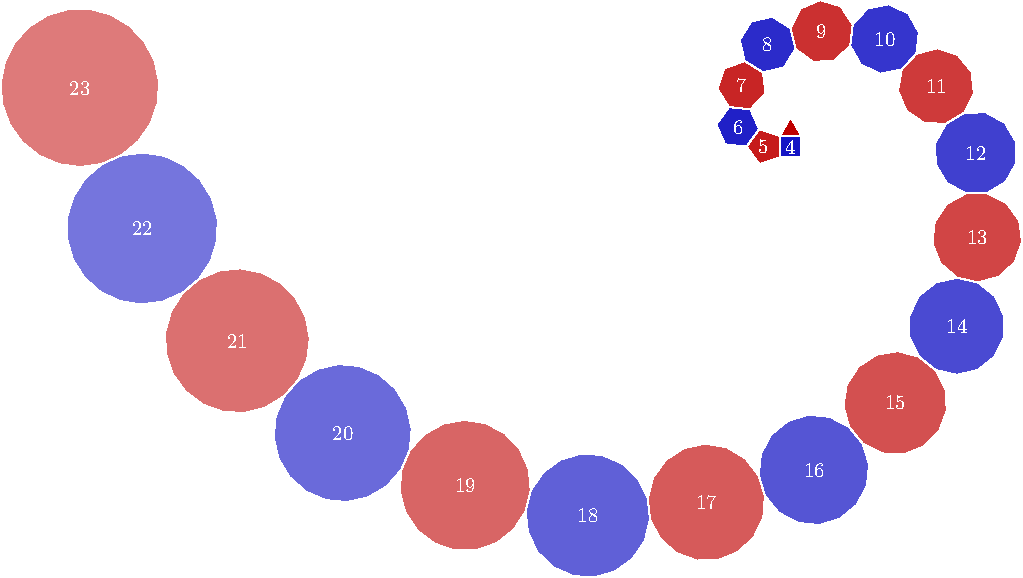
\includegraphics[width=0.9\textwidth]{closed-polygon-chain.pdf}$$
Here is a way to do that using the “\mpl{of}” syntax in the macro construction \rightarrowfill
\vadjust{\moveright 384pt\vbox to 0pt{\vss
\smallmpexternal[firstline=6,lastline=22]{closed-polygon-chain.mp}
\vskip -42pt}}

\newpage\subsection{Curved polygons}

\textsc{The regular polygons} above are all defined with straight edges using the
\mpl{--} connector that makes a tense path.  If you changed each connector to
\mpl{..} you would get a circle, and contrariwise, if you try
\mpl{tensepath(fullcircle scaled 20)} you will get a regular octagon.  But we can
also adjust the directions at the corners to make a variety of closed polygon shapes
with closed edges.  

One of the most pleasing is the Reuleaux polygon, with circular arcs for edges.
$$\includegraphics[width=0.9\textwidth]{closed-reuleaux-set.pdf}$$
The figure on the right attempts to explain the geometry.\mwpic{-160pt}{closed-reuleaux-geometry}
\begin{code}
vardef reuleaux(expr n, r) =
  save a; numeric a; a = 90/n;
  for t = 0 step 4a until 359:
    (0,r) rotated t {left rotated (a+t)} .. {left rotated (3a+t)}
  endfor cycle
enddef;
\end{code}
If you swap the directions at each point you get shapes that are not quite like
hypocycloids; play about a bit more to get flower shapes or windmills.
$$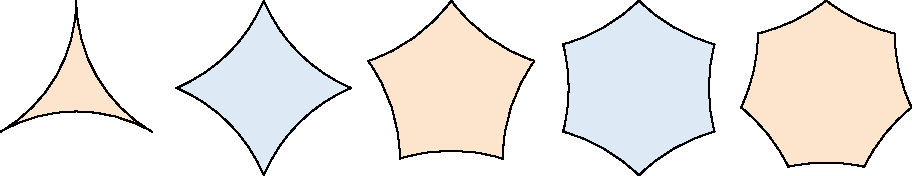
\includegraphics[width=0.9\textwidth]{closed-antireuleaux-set.pdf}$$

\newpage
\subsection{A triangle of Schläfli polygons}\label{sec:gcd}

Apart from the curious polygon patterns in the display, the main \MP\ point of interest
is the recursive "gcd" macro to find the greatest common
divisor.\mpic{-108pt}{closed-schlafli-polygons}

\mpexternal[firstline=6,lastline=26]{closed-schlafli-polygons.mp}

\noindent
The macro also leads directly to an efficient way to find the least common multiple:
\begin{code}
vardef lcm(expr a, b) = a / gcd(a, b) * b enddef;
\end{code}
As always in \MP, it is safer to divide as early as possible to reduce the chance of arithmetic
overflow.


\newpage\subsection{Building cycles from parts of other paths}

Plain \MP\ has a built-in function to compute the intersection points of two paths, and
there’s a handy high level function called "buildcycle" that uses this function to
create an arbitrary closed path.
\mpic{-36pt}{closed-area-under-graph}
The arguments to the function are just a list of paths, and providing the paths all
intersect sensibly, it
returns a closed path that can be filled or drawn.  This is often used for colouring an
area under a function in a graph.
Here is an example. The red line has been defined
as path "f" and the two axes as paths "xx", and "yy".  The light blue area was defined
with
\mpexternal[firstline=18,lastline=18]{closed-area-under-graph.mp}
\noindent
Note the re-use of the $y$-axis path shifted along by different amounts.

\vfill\noindent
There are similar examples in the \MP\ manual, but "buildcycle" can also
be useful in more creative graphics.
Here’s a second example that uses closed paths to give an illusion of depth to a simple
graphic of the planet Saturn.
\mpic{0pt}{closed-saturn}
\marginpar{\hbox{}\vskip1.3in\raggedright\noindent\textbf{Notes}\begin{itemize}
    \item The first five paths are just circles and ellipses based on \mpl{fullcircle}.
    \item The drawing is done inside an \mpl{image} simply so that the final result can
        be drawn at an angle
    \item \mpl{unfill gap} means: \mpl{fill gap withcolor background}
    \item The subpaths passed to \mpl{buildcycle} are chosen carefully to make sure we
        get the intersections at the right points and so that the component paths
        all run in the same direction.  Note that \mpl{subpath (8,4) of globe} runs
        clockwise (that is backwards) from point 8 to point 4.
\end{itemize}}
\mpexternal[firstline=7,lastline=23]{closed-saturn.mp}

\newpage\subsection{The implementation of \texttt{buildcycle}}
\textsc{The implementation} of \mpl{buildcycle} in plain \MP\ is interesting for a number of
reasons.  Here it is copied from "plain.mp" (with minor simplifications) $\longrightarrow$
\vadjust{\moveright5.5in\vbox to 0pt{\kern-1cm%
\begin{code}
vardef buildcycle(text input_path_list) =
  save ta, tb, k, j, pp; path pp[];
  k=0;
  for p=input_path_list: pp[incr k]=p; endfor
  j=k;
  for i=1 upto k:
    (ta[i], length pp[j]-tb[j])
      = pp[i] intersectiontimes reverse pp[j];
    if ta[i]<0:
      errmessage("Paths " & decimal i &
                  " and " & decimal j & " don't intersect");
    fi
    j := i;
  endfor
  for i=1 upto k:
    subpath (ta[i],tb[i]) of pp[i] ..
  endfor cycle
enddef;
\end{code}
\vss}}

\noindent
Notice how freely the indentation can vary; this is both a blessing
(because you can line up things clearly) and a curse (because the syntax may not
be very obvious at first glance).  Notice also the different ways we can use a
\mpl{for}-loop.  The first two are used at the ‘outer’ level to repeat complete
statements (that end with semi-colons); the third one is used at the ‘inner’ level
to build up a single statement.

The use of a \mpl{text} parameter allows us to pass a comma-separated list as an
argument; in this case the list is supposed to be a list of path expressions that
(we hope) will make up a cycle.  The first \mpl{for} loop provides us with a standard
idiom to split a list; in this case the comma-separated value of "input_path_list"
is separated into into a more convenient array of paths called "pp" indexed by "k".
Note that the declaration of the array as \<path> forces the argument to be a list of
paths.

The second \mpl{for} loop steps through this array of paths looking for intersections.
The index "j" is set to be "k" when "i=1", and then set to the previous value of "i"
at the end of the loop;   in this way
"pp[j]" is the path before "pp[i]" in what is supposed to be a cycle.
The macro uses the primitive operator \mpl{intersectiontimes} to find the intersection
points, if any. Note that we are looking for two path times: the time to start a
subpath of the current path and the time to end a subpath of the previous path; the
macro does this neatly
by reversing the previous path and setting the $b$-point indirectly by subtracting
the time returned from the length of the path.

If all has gone well, then "ta" will hold all the start points of the desired
subpaths, and "tb" all the corresponding end points.  The third and final \mpl{for}
loop assumes that this is indeed the case, and tries to connect them all together.
Note that it uses \mpl{..} rather than \mpl{&} just in case the points are not quite
co-incident; finally it finishes with a \mpl{cycle} to close the path even though
point \mpl{tb[k] of pp[k]} should be identical (or at least very close) to point
\mpl{ta[0] of pp[0]}.

This implementation of \mpl{buildcycle} works well in most cases, provided that there
are enough components to the cycle of paths.  If you only have two paths, then the
two paths need to be running the same direction, and the start of each path must not
be contained within the other.  This is explored in the next section.

\newpage
\subsection{Strange behaviour of \texttt{buildcycle} with two closed paths}

The implementation of "buildcycle" in plain \MP\ can get confused if you use it with
just two paths.  Consider the following example: \mpic{0pt}{overlaps-missing-filler}

\mpexternal[firstline=7,lastline=14]{overlaps-missing-filler.mp}

When we compile this example, we get no error message from "buildcycle", but there
is no fill colour visible in the output.  The problem is that the points found by
"buildcycle" are the same both times that it steps through the middle loop, so
the closed path it returns consists of two identical (or very close) points and the
so the fill has zero area.

Now observe what happens when we rotate and reverse each of the paths in
turn.\mpic{-24pt}{overlaps-default-fillers}
Number 1 corresponds to the example shown above; point~0 of~$A$ is inside the closed
path $B$.  In~2 we have rotated path $A$ by 180° so that the start of path~$A$ is no
longer inside $B$, and now "buildcycle" works ‘properly’ --- but this is the only
time it does so.  In~3, we've rotated $B$ by 180° as well, so that $B$ starts inside
$A$ and as expected "buildcycle" fails.  In 4 we've rotated $A$ back to it's
original position, so that both paths start inside each other; and we get the
union of the two shapes.  In 5--8, we've repeated the exercise with path $A$
reversed, and "buildcycle" fails in yet more interesting ways.

You could use this behaviour as a feature if you need to treat $A$ and $B$ as sets
and you wanted to fill the intersection, union, or set differences, but if you just
wanted the overlap, then you need to ensure that both paths are running in the same
direction and that neither of them starts inside the other.

\newpage
\subsection{Find the overlap of two closed paths}

As we have seen, in order to get the overlap of two closed paths from "buildcycle",
we need both paths to be running in the same direction, and neither path should
start inside the other one.  It's not hard to create an "overlap" macro that does
this automatically for us.  The first element we need is a macro to determine if a
given point is inside a given closed path.  Following Robert Sedgwick's
\textit{Algorithms in C} we can write a generic "inside" function that works with any
simple closed path.  The approach is to extend a horizontal ray from
the point towards the right margin and to count how many times it crosses the closed
path; if the number is odd, the point must be inside.\vadjust{\moveright5.5in\vbox
    to 0pt{\kern-4.05cm
\begin{code}
vardef inside(expr p, ring) =
  save t, count, test_line;
  count := 0;
  path test_line;
  test_line = p -- (infinity, ypart p);
  for i = 1 upto length ring:
     t := xpart(subpath(i-1,i) of ring
                  intersectiontimes test_line);
     if ((0<=t) and (t<1)): count := count + 1; fi
  endfor
  odd(count)
enddef;
\end{code}
\vss}}\label{function:inside}

Equipped with this function we can create an "overlap" function that first uses the
handy "counterclockwise" function to ensure the given paths are running in the
same direction, and then uses "inside" to determine where the start points are.
\begin{smallcode}
vardef front_half primary p = subpath(0, 1/2 length p) of p enddef;
vardef back_half primary p = subpath(1/2 length p, length p) of p enddef;
% a and b should be closed paths...
vardef overlap(expr a, b) =
  save A, B, p, q;
  path A, B; boolean p, q;
  A = counterclockwise a;
  B = counterclockwise b;
  p = not inside(point 0 of A, B);
  q = not inside(point 0 of B, A);
  if (p and q):
    buildcycle(A,B)
  elseif p:
    buildcycle(front_half B, A, back_half B)
  elseif q:
    buildcycle(front_half A, B, back_half A)
  else:
    buildcycle(front_half A, back_half B, front_half B, back_half A)
  fi
enddef;
\end{smallcode}
Using this "overlap" macro in place of "buildcycle" produces less surprising
results.\mpic{-2in}{overlaps}

\newpage
\section{Numbers}

This section discusses plain \MP's scalar numeric variables
and what you can do with them.
\MP\ inherits its unusual native system of scaled numbers from \MF;  like many of
Knuth's creations it is slightly quirky, but works very well once you get the hang
of it.  The original objective was to make \MF\ produce identical results on a wide
variety of computers.  By default all arithmetic is carried out using 28-bit
integers in units of $1/65536$.  This is done automatically for you, so you don’t
need to worry about it, but you should be aware of a couple of practical
implications:
\begin{itemize}
    \item All fractions are rounded to the nearest multiple of $1\over65536$, so
         negative powers of 2 ($1\over2$,
        $1\over4$, $1\over8$, $\dots$) are exact, but other common fractions are not:
        for example $1\over3$ is represented as
        ${21845\over65536} \simeq 0.333328$, and $1\over10$ as
        ${6554\over65536} \simeq 0.100006$.
        You should bear this in mind particularly when you
 choose fractional step-values in a "for" loop; the errors can accumulate so that
 you may miss your expected terminal value.\vadjust{\moveright5.5in\vbox to
 0pt{\kern-2in\hsize4in\noindent
        Compare the following two snippets:
     $$\vbox{\halign{#\hfil\quad&#\hfil\cr
     Code&Output\cr\noalign{\smallskip\hrule\bigskip}
\vtop{\begin{code}[xleftmargin=0pt, xrightmargin=160pt]
for i = 0 step 1/10 until 1:
    show i;
endfor
\end{code}}
     &
     \vtop{\parindent0pt\parskip-2pt\obeylines\hsize60pt\ttfamily
>> 0
>> 0.1
>> 0.20001
>> 0.30002
>> 0.40002
>> 0.50003
>> 0.60004
>> 0.70004
>> 0.80005
>> 0.90005
}
\cr\noalign{\bigskip}
\vtop{\begin{code}[xleftmargin=0pt, xrightmargin=160pt]
for i = 0 step 1 until 10:
    show i/10;
endfor
\end{code}}
     &
     \vtop{\parindent0pt\parskip-2pt\obeylines\hsize60pt\ttfamily
>> 0
>> 0.1
>> 0.2
>> 0.3
>> 0.4
>> 0.5
>> 0.6
>> 0.7
>> 0.8
>> 0.9
>> 1
}\cr\noalign{\bigskip\hrule}\cr
}}$$
Unless you run this with "-numbersystem=decimal", you will get
11 iterations in the second but only 10 with the first.
\vss}}

    \item The system limits you to numbers that are less than 4096 in absolute value.
        This can be an irritation if you are trying to plot data with large values,
        but the solution is simple:  scale your values to a reasonable range first.

    \item Intermediate calculations are allowed to be up to 32768 in absolute value
        before an error occurs.  You can sometimes avoid problems by using the
        special Pythagorean addition and subtraction operators, but the general
        approach should be to do your calculations before you scale a path
        for filling or drawing.

    \item You can turn a number up to 32768 into a string using the "decimal"
        command, and then you could append zeros to it using string concatenation.

\end{itemize}

If you are using a recent version of \MP\ you can avoid all these issues by choosing one of
the three new number systems: double, binary, or decimal, with the "numbersystem"
command line switch.  But beware that if you write programs that depend on these new
systems, they might not be so portable as others.  It's nice to have these new
approaches just in case, but you will not need to use them very often.

\newpage\subsection{Numeric constants}

Alongside the quirky number system,
plain \MP\ also inherits three numeric constants from \MF: \id{infinity}, \id{epsilon},
and \id{eps}:
\begin{itemize}
    \item $\id{eps}$ is defined to be a
small amount that is noticeable to \MF’s rounding algorithms, namely
${32\over65536}={1\over2048}\simeq 0.00049$.  As a distance on the page or screen it's invisible at
any resolution less than 150,000 dots per square inch.  If you were designing fonts
        in \MF, $\id{eps}$ could help you avoid bad choices of pixels at low resolutions, but in
\MP\ it's only really useful in comparisons that might suffer from rounding errors.
\id{eps} is tiny, but it's bigger than any rounding error you may encounter, so
you can safely test for equality with: $\kw{abs}(\id{a}-\id{b})<\id{eps}$.

\item $\id{epsilon}$ is defined to be $1\over65536$, the smallest positive scaled
    number.

\item $\id{infinity}$ is defined to be $4096-\id{epsilon}$, which is the largest
    number you will normally deal with. This is useful when you just want a quantity
    larger than any other in the immediate vicinity.  For an example, look at the
    definition of the "inside" function in
    section~\ref{function:inside}.
\end{itemize}
These three quantities retain (approximately) the same value even if you choose one of the
alternative, higher precision, number systems.   This is probably the most sane
approach, but the constants lose their status as the smallest and largest numbers you can
have.
\vadjust{\moveright5.5in\vbox to 0pt{\kern-221pt\hsize 4.25in
\noindent
Running the toy program:
\begin{code}
show numbersystem, eps, epsilon, infinity; end.
\end{code}
gives the following results with the different
number systems:

\begin{code}
>> "scaled"
>> 0.00049
>> 0.00002
>> 4095.99998

>> "double"
>> 0.00048999999999999998
>> 1.52587890625e-05
>> 4095.9999800000001

>> "binary"
>> 0.00048999999999999999999999999999999993
>> 0.0000152587890625
>> 4095.9999800000000000000000000000001

>> "decimal"
>> 0.00049
>> 0.0000152587890625
>> 4095.99998
\end{code}
\vss}}

The messy set of results shown on the right arises because "plain.mp" defines these constants
like this (in version 1.005, which is current at the time of writing):
\begin{code}
eps := .00049;    % this is a pretty small positive number
epsilon := 1/256/256;   % but this is the smallest
infinity := 4095.99998;    % and this is the largest
\end{code}
If you want cleaner constants, feel free to redefine the two decimals as:
\begin{code}
eps := 1/2048;
infinity := 64*64-epsilon;
\end{code}
These definitions are equivalent with "scaled" numbers, but more consistent at
higher precision.  In particular they ensure that we always have
$4096 = \id{infinity} +\id{epsilon}$ whichever number system is in use.

\newpage\subsection{Units of measure}
In addition to the very small and very large numeric variables, plain \MP\ inherits
eight more that provide a system of units of measure compatible with \TeX.
The definitions in "plain.mp" are very simple: $\longrightarrow$
\vadjust{\moveright 384pt\vbox to 0pt{\kern-24pt
\begin{code}
mm=2.83464;      pt=0.99626;        dd=1.06601;      bp:=1;
cm=28.34645;     pc=11.95517;       cc=12.79213;     in:=72;
\end{code}
\vss}}

When the output of \MP\ is set to be PostScript, then the basic unit of measure is
the PostScript point.  This is what \TeX\ calls a "bp" (for `big point'), and it is
defined so that $1\unit{inch}=72\unit{bp}$.  The traditional printers' point, which \TeX\
calls a~"pt", is slightly smaller so that $1\unit{inch}=72.27\unit{pt}$.

Normal use of these units relies on \MP's implicit multiplication feature.  If you write
`$\id{w}=10\,\id{cm};$' in a program, then the variable \id{w} will be set to the value 283.4645.
The advantage is that your lengths should be more intuitively understandable, but if
you are comfortable thinking in PostScript points (72 to the inch, 28.35 to the
centimetre) then there is no real need to use any of the units.\marginpar{Bizarrely, 28.35
is also the number of grammes to the ounce.}

It is sometimes useful to define your own units; in particular many \MP\ programs
define something like `$\id{u}=1\,\unit{cm};$' near the start, and then define all
other lengths in terms of \id{u}.  If you later wish to make a smaller or larger
version of the drawing then you can adjust the definition of \id{u} accordingly.
Two points to note:
\begin{itemize}
    \item If you want different vertical units, you can define something like
        `$\id{v}=8\,{mm}$' and specify horizontal lengths in terms of \id{u}, but
        verticals in terms of \id{v}.
    \item If you want to change the definition of \id{u} or \id{v} from one figure
        to the next, you will either have to use `$\kw{numeric} \id{u},\id{v};$' at
        the start of the your program in order to reset them, or
         use the assignment operator instead of the
        equality operator to overwrite the previous values.
\end{itemize}

The unit definitions in "plain.mp" are designed for use with the default scaled
number system; if you want higher precision definitions, then you can update them by
including something like this at the top of your program: $\longrightarrow$
\vadjust{\moveright 5.5in \vbox to 0pt{\kern-24pt
\begin{code}
% exact values to re-define the plain.mp units
numeric bp, in, mm, cm, pt, pc, dd, cc;
72 = 72 bp = 1 in;
800 = 803 pt = 803/12 pc;
3600 = 1270 mm = 127 cm;
1238 pt = 1157 dd = 1157/12 cc;
\end{code}
%\bgroup\obeylines\parindent0pt
%$\kw{numeric} \id{bp}, \id{in}, \id{mm}, \id{cm}, \id{pt}, \id{pc}, \id{dd}, \id{cc};$
%$72 = 72\id{bp} = 1\id{in}$;
%$800 = 803 \id{pt} = 803/12 \id{pc};$
%$3600 = 1270 \id{mm} = 127 \id{cm};$
%$1238 \id{pt} = 1157 \id{dd} = 1157/12 \id{cc};$
%\egroup
\vss}}

The effect of the $\kw{numeric}$ keyword is to remove the previous definitions; the
four equation lines then re-establish the units with very slightly more accurate
definitions.  You can safely use these definitions with "scaled", as they are
equivalent to the decimals currently given in "plain.mp", but the main point of the
example is to show how you can do implicit definitions with equations.


\newpage
\subsection{Integer arithmetic, clocks, and rounding}

Native \MP\ provides nothing but a "floor" function, but "plain.mp" provides several
more useful functions based on this.
\begin{itemize}
      \item `$\mathop{\kw{floor}} x$' returns $\lfloor x\rfloor$, $\hbox{the
          largest integer} \le x$.  You can use "x=floor x" to check that $x$ is an
          integer.
    \item `$\mathop{\kw{ceiling}} x$' returns $\lceil  x\rceil$,  $\hbox{the
        smallest integer} \ge x$.

    \item `$x \mathbin{\kw{div}} y$' returns          $\lfloor x/y \rfloor$, integer
        division.
    \item `$x \mathbin{\kw{mod}} y$' returns $x-y\times\lfloor x/y \rfloor$,
        integer remainder.

\end{itemize}
Note that $\kw{mod}$ preserves any fractional part, so $355/113 \mathrel{\kw{mod}} 3 = 0.14159$.

\smallskip
\parshape=1 0pt 3.4in
This behaviour is usually what you want.
\vadjust{\moveright 266pt \vbox to 0pt{\noindent  
\begin{mplibcode}
input clocks
draw clock(hour, minute) scaled 0.8;
\end{mplibcode}\vss}}
For example we can use it to turn the time of day into an appropriate rotation for
the hands of a clock.%
\vadjust{\moveright 384pt\vbox to 0pt{\kern-196pt
\mpexternal[firstline=9,lastline=46,xleftmargin=0pt]{clocks.mp}
\vss}}
In the program given on the right, this idea
is used to define functions that convert from hours and minutes
to degrees of rotation on the clock.
\MP\ provides two internal variables
\id{hour} and \id{minute} that tell you the time of day when the
current job started.  The clock face shown here was generated using
$$\kw{beginfig}(1);{}\mathbin{\kw{draw}}\id{clock}(\id{hour},\id{minute}); \kw{endfig};$$
to give a sort of graphical time stamp.

\vfill

There is also a "round" function that rounds a number to the nearest integer.  It is
essentially defined as $\kw{floor}(x+0.5)$ except that it is enhanced to
deal with \<pair> variables as well.  If you round a pair the $x$-part and
the $y$-part are rounded separately, so that $\kw{round}(3.14159, 2.71828)
= (3,3)$.

The "round" function only takes a single argument, but you can use it to round to a
given number of places by multiplying by the precision you want, rounding, and then
dividing the result. So to round to the nearest eighth you might use
`$\kw{round}(x\times8)/8$', and to round to two decimal places
`$\kw{round}(x\times100)/100$'.  The only restriction is that the intermediate value
must remain less than 32767 if you are using the default number system.

\newpage
\subsection{Integer powers}

\textsc{Occasionally} you might get
caught out by the implementation of the \mpl{**} operator.  As the table on the right shows, you may get
an approximate answer from \mpl{x ** y} even when $x$ and $y$ are both integers.
\vadjust{\moveright 384pt\vbox to 0pt{\kern -2pt
$$\begin{mplibcode}
%primarydef x ** y = 1 for n=1 upto y: * x endfor enddef;
for x=1 upto 19:
    for y = 1 upto 7:
        if x = 1:
            label("$x" if y>1: & "^{" & decimal y & "}" fi & "$", (52y, -20x));
        elseif y * mlog(x) < mlog(infinity):
            numeric r; r = x ** y;
            label(decimal r, (52y, -20x)) withcolor 3/4 if r = round(r): blue
            else: red fi;
        fi
    endfor
endfor
label.lft("Results of \mpl{x**y} for small values, using", lrcorner currentpicture shifted 36 up);
label.lft("the default \mpl{scaled} number system", lrcorner currentpicture shifted 24 up);
currentpicture := currentpicture scaled 0.8;
\end{mplibcode}$$\vss}}
Note that the squares are all integers, and the powers of two appear to be ok
(although if the page was wider you would see that \mpl{2**9} is $512.00002$), but
that with a couple of exceptions cubes and higher powers are all slightly off.  Changing
to one of the new number systems makes it worse; even $x^1$ is not always an integer.  The reason
can be found in the way that the \mpl{**} operator is defined in "plain.mp".
\begin{smallcode}[xleftmargin=0pt, xrightmargin=-36pt]
primarydef x ** y = if y = 2: x * x else: takepower y of x fi enddef;
def takepower expr y of x =
  if x > 0: 
    mexp(y * mlog x)
  elseif (x = 0) and (y > 0): 
    0
  else: 
    if y = floor y:
      if y >= 0: 1 for n=1 upto y: * x endfor
      else:      1 for n=-1 downto y: / x endfor
      fi
    else: 
      hide(errmessage "Undefined power: " & decimal x & "**" & decimal y)
    fi 
  fi 
enddef;
\end{smallcode}
This is inherited directly from plain \MF, and as it says in the \mfbook, it is
optimized for $x^2$ and takes care to handle correctly negative numbers and zeros.
But for all positive values of $x$ other than 2 it is implemented using logs, and
the results are therefore only approximate.  To avoid confusion where this might
matter (such as a particular offset into a recursively defined path) you could
simply use \mpl{round(7**3)} to get a whole number, or if you are sure that your $y$
values are all non-negative integers, you could temporarily replace the definition:
\begin{smallcode}
primarydef x ** y = 1 for n=1 upto y: * x endfor enddef;
\end{smallcode}


\newpage
\section{Pairs, triples, and other tuples}

\vpic{7pt}{random-selection}

\noindent
\MP\ inherits a generalized concept of number from \MF\ that includes ordered pairs.
Pairs are primarily used as Cartesian coordinates, but can also be used as complex
numbers, as discussed below.  \MP\ extends this gener\-al\-ization with 3-tuples and
4-tuples.  Just like pairs, the elements in these tuples can take any numeric value,
so in theory it would be possible to use them for three- and four-dimensional
coordinates, but there are no built-in facilities for this in plain \MP, so some
external library is needed.  \textit{All of the various attempts at three dimensions
in \MP\ are rather difficult to use, so none of them is discussed in this document}.

\smallskip\noindent
Unlike simple numerics, the extended tuple variables are not automatically
declared for you, so if you want to define points $A$ and $B$ you need to explicitly
write `$\kw{pair} \id{A},\id{B};$' before you assign values to them.  Once you have
declared them, you can equate them to an appropriate tuple using $=$ as normal.

\begin{code}
    pair A,B; A = B = (1,2);
    color R;  R = (1,2,3);
    cmykcolor C; C = (1,2,3,4);
\end{code}

The normal use of triples and quads is for colours (RGB colours and CMYK colours);
Triples are type \kw{color}, quads are type \kw{cmykcolor}.
You can't have tuples of any other length, not even as constants, except for
transforms.

A transform is how \MP\ represents
an affine transformation such as "rotated 45 shifted (10,20)".
They are represented as 6-tuples, but if you try to write:
\begin{code}
    transform T; T = (1,2,3,4,5,6); % <-- doesn't work
\end{code}
you will get a parsing error (that complains about a missing parenthesis after the 4).
You can examine and assign the individual parts using `$\kw{xpart} \id{T}$' etc.
More details below, and full details in the \MF\ book.


\newpage\subsection{Pairs and coordinates}
Now \textbf{pairs}:  if you enclose two numerics in parentheses, you get a \<pair>.  A
pair generally represents a particular position in your drawing with normal, orthogonal
Cartesian $x$- and $y$-coordinates, but you can use a pair variable for other
purposes if you wish.  As far as \MP\ is concerned it's just a pair of numerics.

\MP\ provides a simple, but slightly cumbersome, way to refer to each half of a
pair.  The syntax `$\kw{xpart} \id{A}$' returns a numeric equal to the first number in
the pair, while `$\kw{ypart} \id{A}$' returns the second.  The names refer to the
intended usage of pair variable to represent pairs of $x$ and $y$-coordinates.
Note that they are read-only; you can't
assign a value to an $\kw{xpart}$ or a $\kw{ypart}$.  So if you want to update only one
part of a pair, you have to do something like this: $\id{A} \mathrel{:}= (42,
\kw{ypart}\id{A});$

In addition there is a neat macro definition in plain \MP\ that allows you do deal
with the $x$- and $y$-parts of pairs rather more succinctly.
\vadjust{\moveright 384pt\vbox to 0pt{\kern-140pt
\noindent Plain \MP\ provides this definition
\begin{code}
vardef z@#=(x@#,y@#) enddef;
\end{code}
which you can use to find orthogonal points.

\bigskip\noindent
\includegraphics{random-function}
\vss}}%
The deceptively simple definition of $\id{z}$ as a subscripted macro allows you to
write "z1 = (10,20);" and have it automatically expanded into the equivalent of
"x1=10;" and "y1=20;".  You can then use "x1" and "y1" as independent numerics or
refer to them as a pair with "z1".  A common usage is to find the orthogonal points
on the axes in graphs, like so $\longrightarrow$

\smallskip
There is also a simple way to write coordinates using a polar notation
using\label{polar}
\mpl{dir}.  This macro is defined so that \mpl{dir 30} expands to \mpl{right rotated
30} and then to \mpl{(1,0) rotated 30}, which becomes \mpl{(cosd(30), sind(30)}
or \mpl{(0.86603, 0.5)}. So to get the polar notation
point $(r,\theta)$, where $r$ is the radius and $\theta$ is the angle in degrees
counter-clockwise from the positive $x$-axis, you can write `\mpl{r * dir
theta}'. As usual, with a constant you can omit the multiplication sign, so `\mpl{2
dir 30}' provides another way to define the point "(sqrt(3),1)".

\smallskip
Plain \MP\ defines five useful pair variables: \id{origin}, \id{right}, \id{up},
\id{left}, and \id{down}.  As so often, Knuth-Hobby definitions in "plain.mp" are
quite illuminating
$\longrightarrow$
\vadjust{\moveright 384pt\vbox to 0pt{\kern-36pt
\begin{code}
% pair constants
pair right,left,up,down,origin;
origin=(0,0); up=-down=(0,1); right=-left=(1,0);
\end{code}
\vss}}%
As you can see, pair variables can be used in implicit equations.

They can also be scaled using implicit multiplication, so writing
`$144 \id{right}$' is equivalent to writing `$(144,0)$' but possibly a bit more
readable.  In particular the idiom `$\kw{shifted} 200 \id{up};$'
works well when applied to a point, a path,
or an image.
Unfortunately, this convenient notation does not work well with units of
measure.  This is because implicit multiplication only works between a numeric constant and a
variable.  So `$2 \id{in}\, \id{right}$' does not work as you might expect; you can
write `$2\id{in} \mathrel{\ast}\id{right}$' but by that stage it's probably simpler to
write `$(2\id{in},0)$' or even just `$(144,0)$'.


\newpage
\subsection{Pairs as complex numbers}

As you might expect in a language designed by mathematicians, \MP's pair variables
work rather well as complex numbers.  To represent the number $3+4i$ you can write
"(3,4)".  To get its modulus, you write "abs (3,4)" (which gives $5$ in this case),
and to get its argument, you write "angle (3,4)" (which gives $53.1301$).  Note that
"angle" returns the argument in degrees rather than radians, and that the result is
normalized so that $-180 < \kw{angle} (x,y) \le 180$.

The standard notation for points supports this usage.  You can write "z0=(3,4);" and then
extract or set the real part with "x0" and the imaginary part with "y0".  If you
want to use other letters for your variable names, you can use "xpart" and "ypart"
to do the same thing. So after `\mpl{pair w; w=(3,4);}' you can get the real part with
"xpart w" and the imaginary part with "ypart w".
You can also use the polar notation shown above to write complex numbers.  For
$re^{i\theta}$ you can write `\mpl{r * dir theta}' where "r" is the modulus and
"theta" is the argument in degrees.

The predefined constants \mpl{up},
\mpl{down},
\mpl{left}, and
\mpl{right} also provide points on the unit circle corresponding to $i$, $-i$,
$-1$, and $+1$ respectively.  It's tempting to define `\mpl{pair i; i=(0,1);}', so that
you can write constants like "4i" directly, but this is not very helpful, because
"3+4i" will give you an error since \MP\ does not let you add a "numeric" to a "pair".

However \MP\ does let you add (and subtract) two pairs, so complex addition and
subtraction are just done with the
normal operators.
\vadjust{\moveright 384pt\vbox to 0pt{\vskip -3.74in
$$\includegraphics{complex-operators}$$
\mpexternal[firstline=6,lastline=30]{complex-operators.mp}
\vss}}%
To get the complex conjugate you
could use "reflectedabout(left,right)", but it's probably easier just to write
"(x0,-y0)" or define a simple function:
\begin{code}
    def conj(expr z) = (xpart z, -ypart z) enddef;
\end{code}
Complex multiplication is provided as part of the core language by the "zscaled"
operator.  This is defined with the same precedence as "scaled" or normal scalar
multiplication (which is what you usually want).  So "(3,4) zscaled (1,2)" gives
"(-5,10)" because $(3+4i)\times(1+2i) = 3+6i+4i-8 = -5+10i$.
"zscaled" is only defined to work on two "pair" variables, so you can't write
\mpl{(3,4) zscaled 4}.  To get that effect with "zscaled" you would have to write
\mpl{(3,4) zscaled (4,0)}, but this is the same as
\mpl{(3,4) scaled 4}, which is usually simpler to write.  If your pair is
stored as a variable you can write (for example) \mpl{4 z0} to get the same
effect.  Or \mpl{1/4 z0} or \mpl{z0/4} for scalar division.

There are no other complex operators available, but it is not hard to implement the
usual operations when they are required\dots

\newpage
\subsubsection{Extra operators for complex arithmetic}

Since multiplication by $z$ can be thought of as a transformation consisting of
rotation by the argument of $z$ and scaling by $|z|$, you can define the complex
inverse and complex square root simply using \mpl{angle} and \mpl{abs}.
\vadjust{\moveright5.5in\vbox to 0pt{\hsize4in\vskip -84pt
\centerline{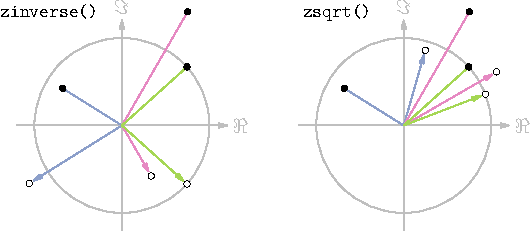
\includegraphics{complex-inverse-and-sqrt}}
\noindent
The drawing uses the two functions defined on the left.
\smallmpexternal[firstline=11,lastline=44,xleftmargin=0pt]{complex-inverse-and-sqrt.mp}
\vss}}

\smallskip\noindent
First an inverse function.  The idea here is to find a function that is the opposite
of complex multiplication, so we want something that gives
\begin{code}
z zscaled zinverse(z) = (1,0)
\end{code}
In other words you need to find a complex number with an argument that is the
negative of the argument of $z$ and a modulus that will scale $|z|$ to 1.
You can use the polar notation with "dir" to write this directly:

\mpexternal[firstline=6,lastline=6]{complex-inverse-and-sqrt.mp}

The complex division, $z/w$, can now be done as: \mpl{z zscaled zinverse(w)}.
The only difficulty with this function is how it deals with zero, or rather with
the point $(0,0)$.  Since `\mpl{abs (0,0)}' gives $0$, the function will give you
a `divide by zero' error if it's called with $(0,0)$.  But this is probably what you want
it to do, since there is no easy way to represent the point at infinity in the
extended complex plane on paper.

\medskip\noindent
For square root, you want a function `\mpl{zsqrt(z)}' that returns
a complex number with half
the argument of $z$ and a modulus that is the square root of the modulus of $z$, so that
`\mpl{zsqrt(z) zscaled zsqrt(z) = z}'.  This does the trick:
\begin{code}
def zsqrt(expr z) = sqrt(abs z) * dir 1/2 angle z enddef;
\end{code}
This function also has a difficulty with the point $(0,0)$, because "angle (0,0)" is
not well defined, and so \MP\ throws an error.  If you want a function that
correctly returns $(0,0)$ as its own square root, then try something like this:
\mpexternal[firstline=7,lastline=9]{complex-inverse-and-sqrt.mp}

\newpage
\subsubsection{Using complex numbers to draw fractals}

As an example of what you can do with complex arithmetic, here is a version of the
diagram from §4.1 of Knuth's \textsl{Seminumerical Algorithms} showing $S$, the set
of all points that can be written as $\sum_{k\ge1}a_k(i-1)^{-k}$.
\vadjust{\moveright5.5in\vbox to 0pt{\hsize4in\vskip -36pt
\mpexternal[firstline=7,lastline=42,xleftmargin=0pt]{double-dragon.mp}
\vss}}
$$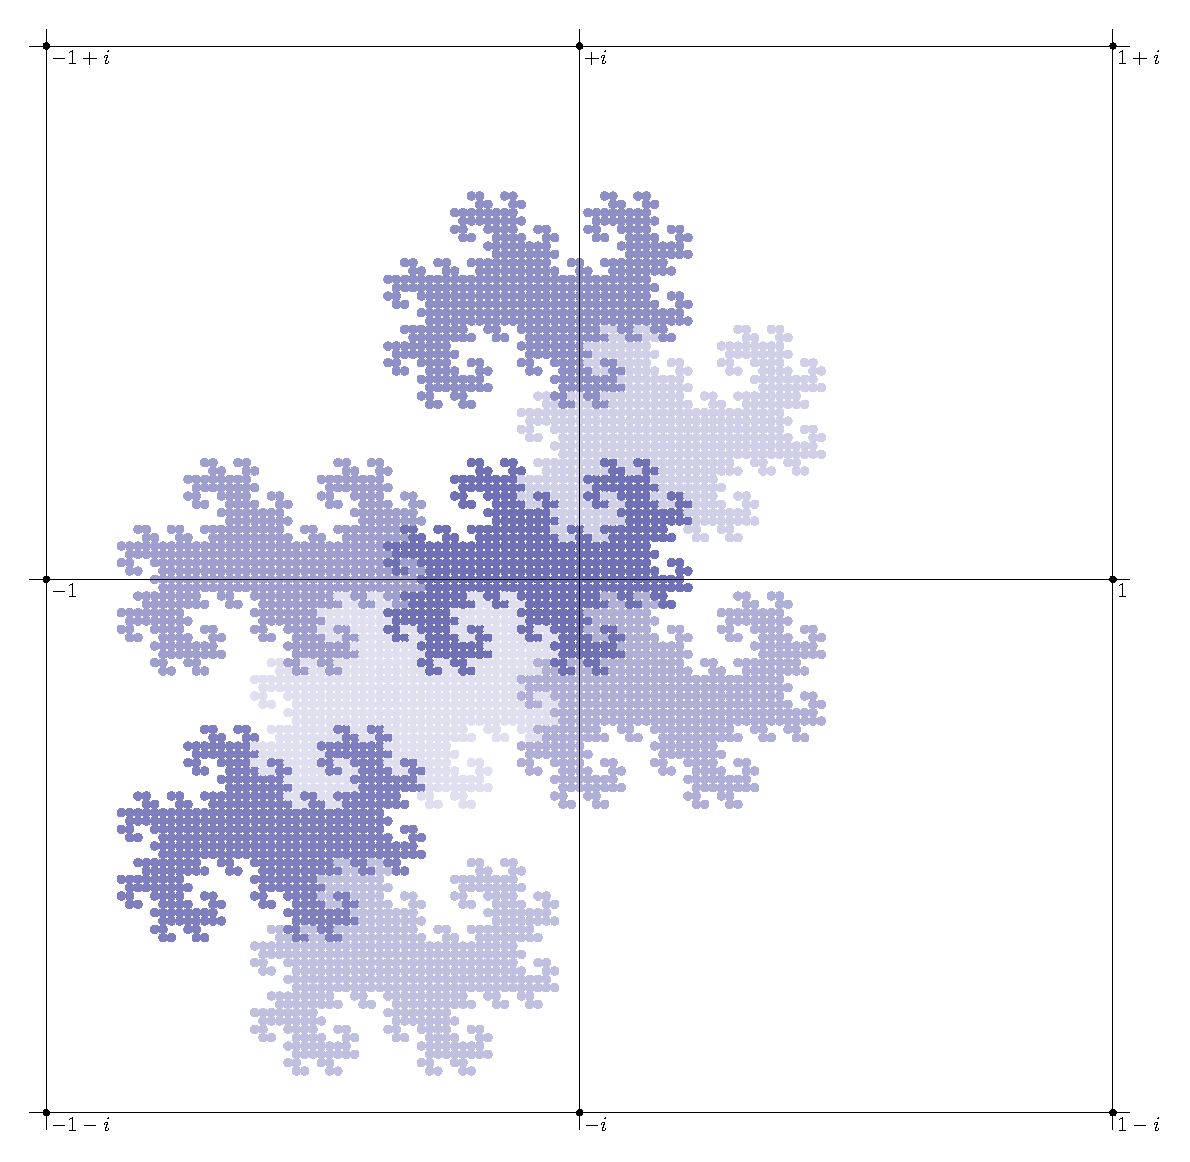
\includegraphics[width=\textwidth]{double-dragon.pdf}$$
\vbox to 0pt{\noindent\small\textbf{Note}: you can adjust the “resolution” with the parameter $t$, but don't
make it smaller than 1 if you are using the default number system; the diagram looks
a bit strange unless $t$ is an integer power of 2.\vss}

\newpage
\section{Colours}

\MP\ implements colours as simple numerics, or tuples of three or four numeric values.
Three-tuples (which are type \mpl{color}) represent RGB colours; four-tuples
(which are type \mpl{cmykcolor}) represent CMYK colours.  Simple numerics are used to
represent grey scale colours.

The numeric values of the colours can take any \kw{numeric} value, but \MP\ only considers the
range 0 to 1 ---  values less than zero are treated as zero, values greater than 1 are
treated as 1.
So British Racing Green with RGB code "(1,66,37)",
or Pillar Box Red with code "(223,52,57)", can be defined like this:
\begin{code}
    color brg, pbr;
    brg = (0.00390625, 0.2578125, 0.14453125);
    pbr = (0.87109375, 0.203125, 0.22265625);
\end{code}
or, slightly more idiomatically:
\begin{code}
    brg = 1/256 (1, 66, 37);
    pbr = 1/256 (223, 52, 57);
\end{code}
As you can see, you can apply implicit multiplication to a \mpl{color}, so after
the declaration above "2 brg" would be a valid colour, although you have to think
a bit to know what that means in terms of colour in your drawings.
\vadjust{\moveright 396pt\vbox to 0pt{\kern-144pt\noindent
To use RGB hex strings, you'll need to write a function:
\begin{code}
vardef hexrgb(expr Spec) =
  save r, g, b;
  numeric r, g, b;
  r = hex substring (1,3) of Spec;
  g = hex substring (3,5) of Spec;
  b = hex substring (5,7) of Spec;
  1/256(r,g,b)
enddef;
brg = hexrgb("#014225");
pbr = hexrgb("#df3439");
\end{code}
\noindent\hey The \mpl{hex} function is a built-in primitive operation.
\vss}}%

Plain \MP\ defines five basic colour constants: \mpl{red}, \mpl{green},
\mpl{blue}, \mpl{white}, \mpl{black}.  These are quite useful with leading
fractions: \mpl{2/3 red} gives a nice dark red, that's good for drawing lines you
want to emphasize; \mpl{1/2 white} gives you a shade of grey; and so on.  But since
\mpl{black} is defined as \mpl{(0,0,0)}, \mpl{1/2 black} just gives you \mpl{black}.

You can also add up \mpl{colors}.  So \mpl{red + 1/2 green} gives you a shade of
orange;  this is more long-winded than writing \mpl{(1, 0.5, 0)} but maybe slightly
easier to read.  Much more usefully, you can use the mediation notation to get a
colour that is part way between two others.  So \mpl{1/2[red, white]} gives you a
shade of pink, and \mpl{2/3[blue, white]} a sort of sky blue.  You can also use this
idea to vary colour with data, as in \mpl{(r)[red, blue]} where \mpl{r} is some
calculated value.  \vadjust{\moveright 396pt\vbox to 0pt{\kern-64pt
\mpexternal[firstline=6,lastline=18]{color-blend-toy.mp}
\vss}}
Here's a toy example:

\vbox to 0pt{\centerline{\includegraphics[scale=0.8]{color-blend-toy}}\vss}

\newpage
\subsection{CMYK colours}

\MP\ also implements a CMYK colour model, using tuples of four numerics.
In this model the four components represent cyan, magenta, yellow, and black.
White is \mpl{(0,0,0,0)} and black is anything where the last component is 1.

Beware that the five colour constants defined in "plain.mp" are defined as RGB
colours, and you can't mix colour models, so anything like \mpl{1/2[(1,1,0,0),
white]} will not work, unless you redefine the color constants as CMYK colours:
\begin{smallcode}
cmykcolor black, white, red, green, blue;
black = (0,0,0,1); white = (0,0,0,0);
red = (0,1,1,0); green = (1,0,1,0); blue = (1,1,0,0);
\end{smallcode}
$$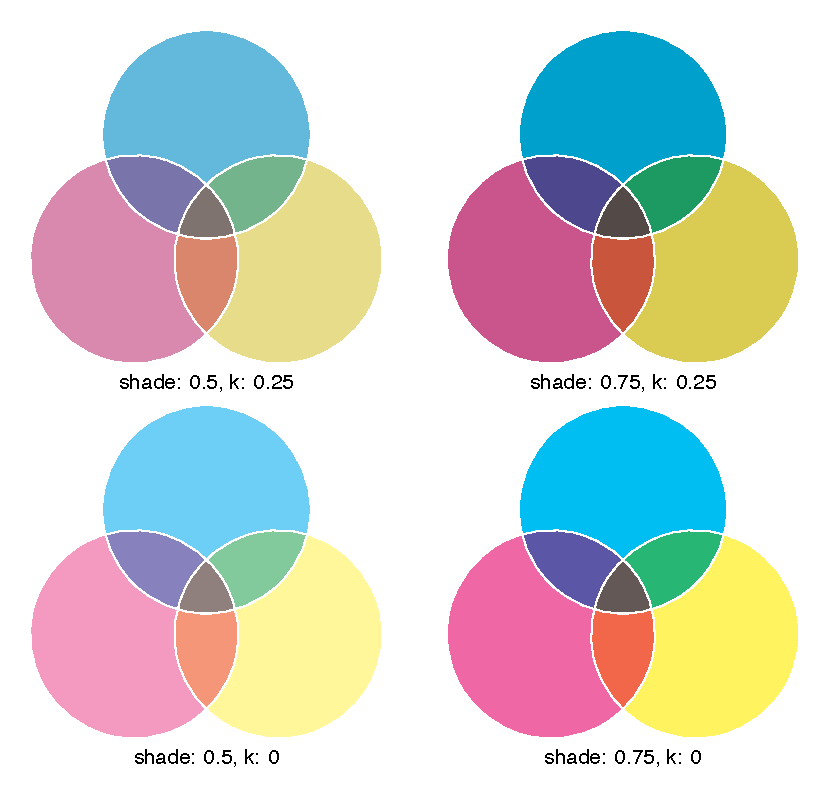
\includegraphics[width=0.7\textwidth]{blended-color-circles}$$
\hey The apparent blending of colours here is done by calculating the overlaps
and filling them in order.  With plain "mpost", there is no support for transparency in any of the
colour models; but "luamplib" gives you access to PDF transparency, see
§\ref{sec:transparent}.

\moveright 384pt\vbox to 0pt{\vss
\mpexternal[firstline=9,lastline=41]{blended-color-circles.mp}
}
\newpage
\subsection{HSV colours}

HSV colours are colours defined by a triple of hue, saturation, and value.
Unlike RGB and CMYK colours there is no native support in \MP\ but it is possible to
write a routine that maps HSV triples into RGB colours:
\mpexternal{color-hsv-macro.mp}
\noindent
This is based on information from the Wikipedia article on
on “HSL and HSV”.

\medskip\noindent
The hue values in HSV colours map nicely to the familiar spectrum
of the rainbow.  In the model used here 0 is red, 120 green, and 240 blue:
$$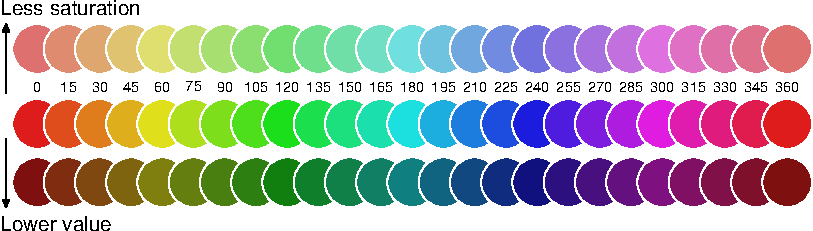
\includegraphics[width=0.85\textwidth]{color-hsv-gamut}$$
With less saturation the colours look faded; if you lower the value they get
darker.  Once you get the hang of them, they make choosing colours rather easier.
You can produce ranges of colour by changing hue, or make gradations of a single
colour by changing the saturation or value.

\moveright 376pt\vbox to 0pt{\vss
\mpexternal[firstline=5,lastline=31]{color-hsv-gamut.mp}}

\newpage
\subsection*{An HSV example of a graduated scale}

\noindent
This example requires the \mpl{hsv_color} macro from the previous page.
\mpic{2pt}{color-hsv-bathymetric}
\mpexternal[firstline=7,lastline=39, xleftmargin=0pt]{color-hsv-bathymetric.mp}

\newpage
\subsection{Grey scale}

\moveright5.4in\vbox to 0pt{\vskip6pt
\mpexternal[firstline=5,lastline=36,xleftmargin=0pt]{color-grey-escher.mp}
\vss}
\noindent
The \mpl{withcolor} command will also take a single \mpl{numeric} instead of a 3-tuple or
a 4-tuple.  This produces a colour in grey scale (or gray scale if you prefer the
Webster spellings).  Just as for the other colour types, values below 0 count as
zero and values above 1 count as one.  And since the smallest possible positive
number in plain \MP\ is: $\id{epsilon} = 1/256/256;$ then you can have at most 65,536 shades in
between.

Grey scale is appropriate for some printed media, and can make effective textures
and patterns. The pattern below was produced by this program \rightarrowfill
$$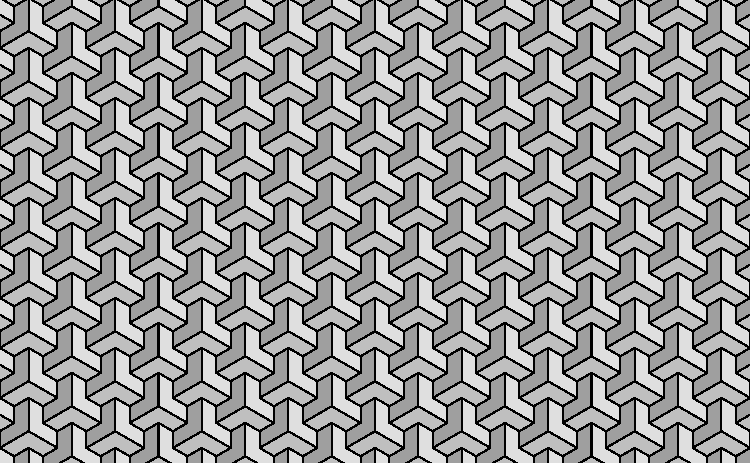
\includegraphics{color-grey-escher}$$
First a basic path (named $\id{atom}$) is defined, then in the first loop three
picture variables, $p_1$, $p_2$, and $p_3$, are defined, each one rotated
120° from the previous and filled with a slightly darker shade of grey.
The double loop then draws the three versions of the shape on an up-and-down grid.
Finally the picture is clipped to a neat rectangle.

\newpage
\subsection*{Drawing algorithmic shadows}
\moveright5.25in\vbox to 0pt{\vskip6pt
\mpexternal[firstline=5,lastline=32]{color-grey-shadows.mp}
\vss}
\noindent
Here is a more complex pattern, showing one way to create an
illusion of shadows with multiple fine lines.
$$
\includegraphics{color-grey-shadows}$$
The first part defines two wedge-shaped closed paths, $\id{w}$ being
the mirror image of $\id{b}$.  Like the standard \id{unitsquare} path, the
path $\id{b}$ is defined so that point 0 is the bottom left corner.

The two \<picture> variables are produced by drawing lines across the shapes from
bottom to top.  If you set the loop step small enough, these multiple lines blend smoothly to
give an even colour.  And by using higher powers of the index variable, an effective
shadow can be drawn ‘bunched up’ into the top of each shape.  Note that \MP\ likes
integer powers of two.

By repeating them alternately in a grid, we get an effective texture, which is
clipped at the end to a neat rectangle again.


\newpage
\subsection{Colorbrewer palettes}\label{colorbrewer}

\moveright 384pt\vbox to 0pt{\vskip144pt\raggedright\hsize4in\noindent
This map shows the "RdYlBu[9]" palette in action on a map of the Brexit vote in
London.  The outlines are the 33 London boroughs, and the colours show how we voted.
The size of the labels shows the turnout.  The data and the outlines are from
public domain sources.  They were prepared for \MP\ using various scripts, 
and they are available in the source for this document.

\vskip 48pt
Here is the code for the palette used as the legend:
\mpexternal[firstline=9,lastline=9]{color-brexit-map.mp}
\mpexternal[firstline=11,lastline=19]{color-brexit-map.mp}
\vss}

\noindent
The well-known Colorbrewer website ("http://colorbrewer2.org") provides a useful set
of colour palettes that are suitable for a wide range of applications.  They were
originally written for maps, but they are useful for many other types of drawing.
If you are using an up-to-date, and complete, \TeX\ distribution, you should find
that my implementation of them for \MP\ is already installed on your system,
otherwise you can get it from "https://ctan.org/pkg/metapost-colorbrewer".  The
package provides two files that define all the colour ranges; one for CMYK and
another for RGB; an example of usage is shown below on the right.

$$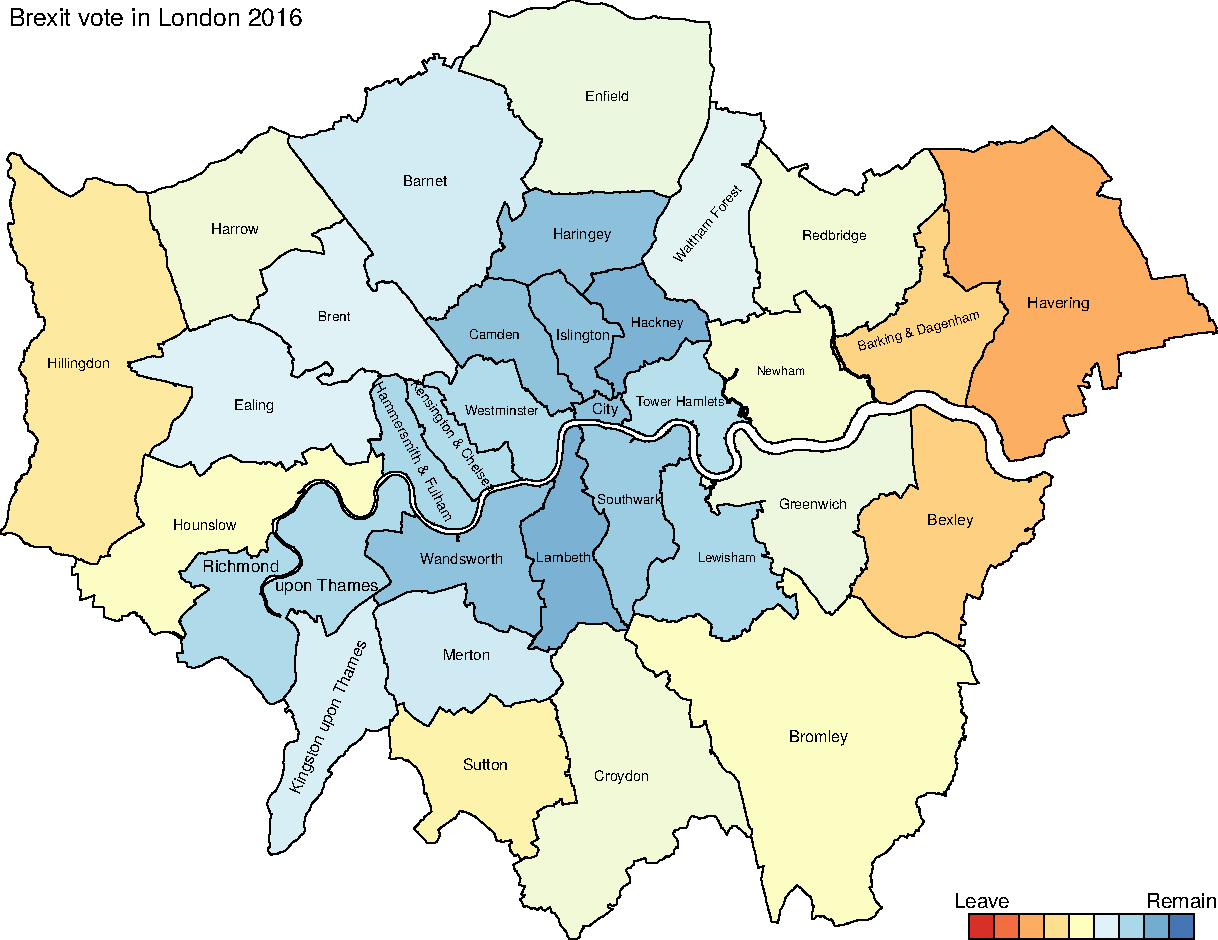
\includegraphics[width=\textwidth]{color-brexit-map.pdf}$$


%--------------------------------------------
\newpage
\section{Random numbers}

\MP\ provides us with two built-in functions to generate random numbers.
\vadjust{\moveright 372pt\vbox to 0pt{\kern-24pt
\mpexternal[firstline=5,lastline=39,xrightmargin=-36pt]{random-dice.mp}
$$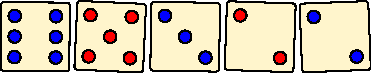
\includegraphics{random-dice}$$
\vss}}
\begin{itemize}
    \item `$\kw{uniformdeviate}\,n$' generates a random real number between $0$ and
        $n$.

        Note that the $n$ is required.  It can be negative, in which case you get negative random
        numbers; or it can be zero, but then you just get $0$ every time. In other words the
        implementation generates a number $r$ such that $0\le r<1$ and then
        multiplies $r$ by
        $n$.

        If you want a random whole number, use `$\kw{floor}$' on the result.
        So to simulate six-sided dice, you can use `$1+\kw{floor}\,\kw{uniformdeviate}6$'.

        If you use the new number systems, and you find that the numbers generated
        are all multiples of $n/4096$, so $\kw{uniformdeviate} 8192$ (for example)
        generates even integers instead of random real numbers, then you should
        update your \TeX\ distribution.  This `feature' was an accident of the
        original way that the scaled arithmetic routines were adapted.

    \item `\kw{normaldeviate}' generates a random real number that follows the
        familiar normal distribution. The algorithm used is discussed in \textsl{The
        Art of Computer Programming}, section~3.4.1.
        If you generate enough samples, the mean should
        be approximately zero, and the variance about 1.
        The chance of getting a number between $-1$ and 1 is
        about 68.3\%; between $-2$ and 2, about 95.4\%.
        \vadjust{\moveright 3.6in\vbox to 0pt{\hsize 1.6in \vskip21pt \noindent
        \small 10000 samples suggest\\\kw{normaldeviate} works.\par\vss}}
        $$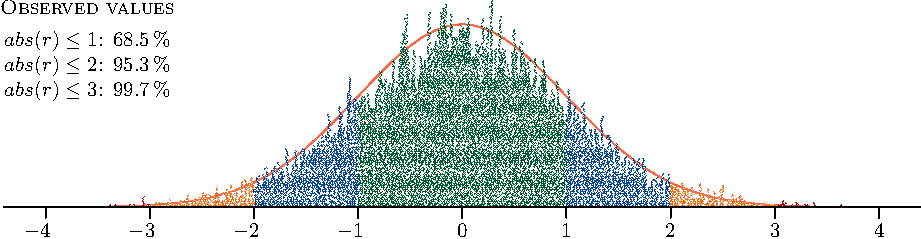
\includegraphics[width=4.6in]{random-gaussian}$$
        To relocate the mean, just add a constant.  To rescale the distribution,
        multiply by the desired standard deviation (the square root of the
        desired variance).


\end{itemize}


\newpage\subsection{Random numbers from other distributions}

The \kw{normaldeviate} function is provided as a primitive \MP\ operation. The
implementation is based on the `Ratio method' presented in \textsl{The Art of
Computer Programming}, section~3.4.1.   It turns out to be very straightforward to
implement the algorithm for this method as a user-level program $\longrightarrow$
\vadjust{\moveright5.5in\vbox to 0pt{\kern -112pt
\smallmpexternal{random-other-distributions.mp}    
\vss}}%

This version of \mpl{normaldeviate} is of academic interest only, in all real code
you should use the primitive operation, but there are a couple of programming notes.
If you put ‘\mpl{u = uniformdeviate 1}’, then you have $0 \le u < 1$, so $v/u$ might
give you a divides-by-zero error; using ‘\mpl{u = 1 - uniformdeviate 63/64}’ ensures
that $1/64 < u \le 1$, which not only avoids the possibility of a divide-by-zero
error, but also ensures that $|(v/u)| < 64$, so that you can square it without
overflow.  This is a useful general technique, and justified in terms of the
algorithm since large values of $v/u$ are rejected anyway.  Secondly, the expression
\mpl{sqrt(8/mexp(256))} is a constant ($ \sqrt{8/e} \simeq 1.71553 $) and could be
replaced by its value, but this does not make an appreciable improvement to the
speed of the routine.  On a modern machine, this routine is only very slightly
slower than using the primitive function.

\medskip\noindent
It is also fairly straightforward to implement random number generators that follow other statistical
distributions.  The mathematical details are in the section of \textsl{TOACP}
referenced above. Two examples, for the exponential distribution and the gamma
distribution, are shown on the right.  In both cases, note the care required to avoid
arithmetic overflow with the default scaled number system.

\medskip\label{mexp}\noindent
You can also see the special nature of \MP's \kw{mexp} and \kw{mlog}
functions. They are defined so that $\kw{mexp} x = \exp(x/256)$ and $\kw{mlog} x =256\log(x)$.
This is another artefact of the scaled number system.  \MP\ computes $x^y$ using the
formula \mpl{mexp(y*mlog(x))}, and the adjusted log values give more accurate results.
Note that this means that you have $e=\kw{mexp}(256)$.

It is sometimes useful to define macros for the usual versions of $\exp$ and $\log$
as shown on the right.   This not only helps you make fewer programming mistakes, and 


\newpage\subsection{Random walks}

You can use the random number generation routines to produce visualizations of
random walks, with various levels of analysis.
\vadjust{\moveright5.5in\vbox to 0pt{\hsize 4.4in\kern -2\baselineskip
\mpexternal[firstline=5,lastline=31,xleftmargin=0pt]{random-walks-red-blue.mp}
\smallskip\noindent
\hey Note the \mpl{undraw} line using a slightly thicker pen; this makes it 
easier to follow the lines as they cross each other.
\vss}}
$$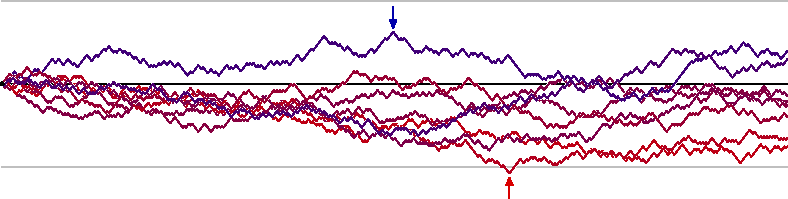
\includegraphics[width=\textwidth]{random-walks-red-blue}$$
In this example the random walk lines are coloured according to the final $y$-value,
and the global maximum and minimum points are marked.

Each walk is created with an `inline' for-loop; the loop is effectively expanded
before the assignment, so that each \id{walk} variable becomes a chain of connected $(x,y)$
pairs.  Inside the loop you can conceal yet more instructions in a `\kw{hide}' block.
These instructions contribute nothing to the assignment, but can change the values
of variables outside the block.

Note the first line of the \kw{hide} block adds $\pm1$ to $y$ with equal probability.
You can (of course) create different kinds of random walks, by changing the way you
set this delta value, for example by using a different type of random variate, or scaling
the value, or changing the odds in favour of one direction or the other.  For
example:
\begin{code}
y := y if uniformdeviate 1 < p: + 2 else: - 1 fi; 
\end{code}
will set the delta to $+2$ with probability $p$ and and to $-1$ with probability $1-p$.

\newpage
\subsubsection{Random walks with different constraints}

\textsc{Formally}, a random walk is constrained to move one unit at a time, but if you relax
that constraint and use `\kw{normaldeviate}' in place of `\kw{uniformdeviate}' you
may get more “realistic” patterns.
\vadjust{\moveright5.5in\vbox to 0pt{\hsize 4.2in\kern2\baselineskip\noindent
The drawing here is much the same as the previous page, except that the definition of
\id{walk} in the central loop is simplified to this:
\mpexternal[firstline=15,lastline=18,xleftmargin=0pt]{random-walks-normal.mp}
}}
$$\includegraphics[width=\textwidth]{random-walks-normal}$$
Alternatively you could add an extra constraint that the final value should be zero
(or some other desired target value); this is the so-called “brownian bridge”.
$$\includegraphics[width=\textwidth]{random-walks-normal-bridge}$$
To do this, you make a random walk path, as above, with \id{n} points, and then copy
it into a new path where the $i$-th point is adjusted by $i/n\times(t-y)$ where $t$
is the target value, and $y$ is the $y$-value of the last point on the walk path.
\vadjust{\moveright5.5in\vbox to 0pt{\hsize 4.2in\vss
\mpexternal[firstline=7,lastline=23,xleftmargin=0pt]{random-walks-normal-bridge.mp}
}}

\newpage\subsection{Brownian motion}

Relaxing all the contraints, can give you even more
interesting patterns.\vadjust{\moveright5.5in\vbox to 0pt{
\hsize4.2in\vskip -32pt
\mpexternal[firstline=6,lastline=20,xleftmargin=0pt]{random-two-dimensional-brownian.mp}

\kern 84pt
\noindent
Using these random number generators means that the output is
different each time because \MP\ produces a different sequence of numbers.  You may
find yourself running the program a few times until you find one you like. At this
point you will wish that you knew what "randomseed" had been used, so that you can
re-create picture.  Unfortunately \MP\ does not log the value used, unless you set it
manually.  So here's a trick to use in this situation: set your own random seed
using a random number at the top of your program.
\begin{code}
    randomseed := uniformdeviate infinity;
\end{code}
Now \MP\ writes the (random) value used in the log for you to copy. Note that if you are using
"luamplib" you need to add the "\mplibshowlog{enable}" option to get this value in
the log.
\vss}}
If you also allow the $x$-coordinates to
wander at random as well as the $y$-coordinates you get two-dimensional random
patterns.  And if you replace the straight line segments "--" with ".." so that \MP\
draws a smooth curve through the points, then the result is almost artistic.

\vbox to 0pt{\noindent
\hbox to \textwidth{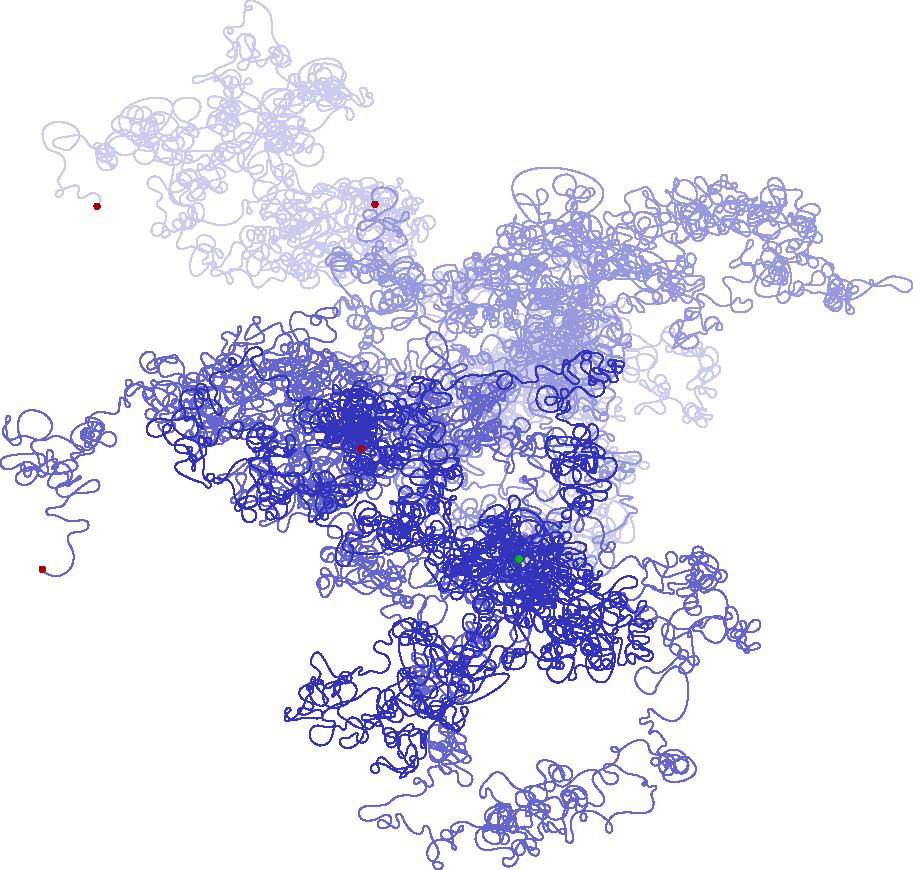
\includegraphics[width=1.2\textwidth]{random-two-dimensional-brownian}\hss}
\vss}

\newpage\subsection{Drawing freehand}

This idea is shamelessly stolen from the wonderful collection of \MP\ examples
available at "http://melusine.eu.org/syracuse/metapost/".  But since the
examples there are all in French (including all the names of the custom macros),
perhaps it would be better to say `translated' rather than `stolen';  moreover my
implementations are easier to use with plain \MP.\vadjust{\moveright5.5in\vbox to 0pt{
\hsize4in\kern -5.5\baselineskip
\smallmpexternal[firstline=5,lastline=42,xleftmargin=0pt]{random-freehand-circumcircle.mp}
\vss}}

\subsubsection{Making curves and straight lines look hand drawn}

$$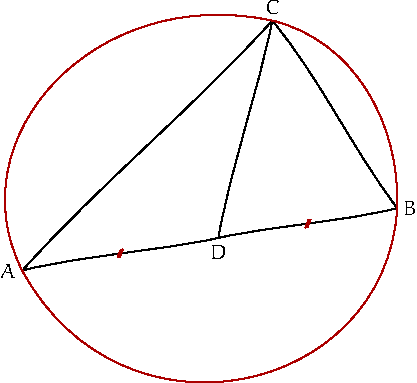
\includegraphics{random-freehand-circumcircle}$$
A small amount of random wiggle makes the drawing come out charmingly wonky.  Notice
that the "freehand_path" macro will transform a path whether it is straight or curved,
and open or closed.  Notice also that to find $D$ the mid-point of a $AB$, you need
to find the
point along the freehand path; if you simply put "1/2[A,B]" there's no guarantee
that the point would actually be on the free hand path between $A$ and $B$.  In this
case a little extra randomness has been added, and the
two segments $AD$ and $DB$ have been marked with traditional
markers to show that they are equal.  The "moved_along" macro combines shifted and
rotating to make the markers fit the wonky lines properly.
The Euler font complements the hand-drawn look; but
you might find that a little of this type of decoration goes a long way.

\newpage
\subsubsection{Extending straight lines slightly}\label{euler}

This second freehand figure uses a macro to draw a wonky line through two points
with a bit of overlap at each end.  The overlap size is given using the suffix
syntax.  The lines are drawn in sepia ink to enhance the hand-drawn look. The angle 
labels are positioned on invisible arcs between neighbouring wonky lines.
\vadjust{\moveright5.5in\vbox to 0pt{
\hsize4in\kern -4.5\baselineskip
\mpexternal[firstline=5,lastline=41,xleftmargin=0pt]{random-freehand-through.mp}
\vss}}

$$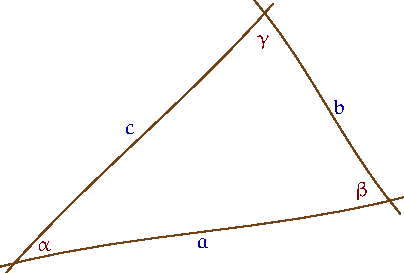
\includegraphics{random-freehand-through}$$

\vfill
\noindent\llap{\nb\ }The AMS Euler font available to \MP\ as "eurm10" is encoded as a subset of the \TeX\
math italic layout --- essentially it has all the Greek letters but none of the
arrows, nor the musical notation.
$$\includegraphics{euler-sampler}$$
If you can't get the upper case $\Gamma$ at \mpl{char 0}, then you might be running 
an old out-of-date version of "luamplib".

\newpage\subsection{Increasingly random shapes of the same size}

If you want a random-looking shape, the general approach is to find a method to make
a path that allows you to inject some random noise at each point of the path.
$$\hbox to \textwidth{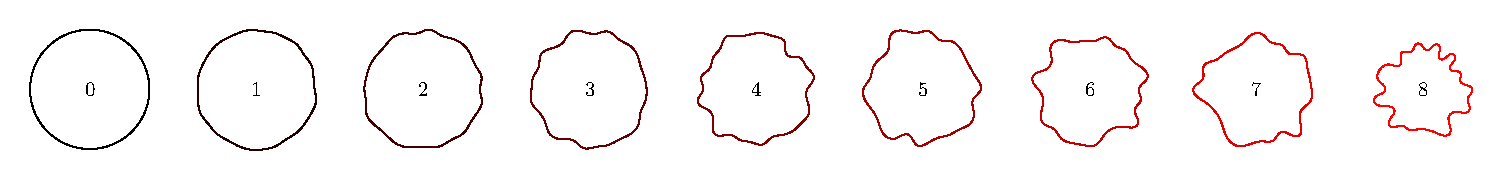
\includegraphics{random-shapes}\hss}$$
For these shapes the objective was to make them increasingly random, but to keep
them all the same length.\vadjust{\moveright5.5in\vbox to 0pt{
\hsize4in
\mpexternal[firstline=6,lastline=21,xleftmargin=0pt]{random-shapes.mp}
\vss}}
Each time round the outer loop the \id{shape} is redeclared to clear it, and
then redefined by an inline-loop with $n$ steps like
this:
\begin{code}
shape = for i=1 upto n: (s,0) rotated (360/n*i) .. endfor cycle;
\end{code}
except that some random noise is added to the $s$ at each step: when the noise is
zero ($\id{r}=0$) you get a circle; as the noise increases the circle is
increasingly distorted.

The scaling is done using the \mpl{arclength} operator.  This works like
\mpl{length} but instead of telling you the number of points in a path, it returns
the actual length as a dimension.  Dividing the desired length by this dimension
gives the required scaling factor for the random shape just defined.  Notice that
you have to do this in two steps, and update the shape using ":=".  This is because
you need to have defined \id{shape} before you can refer to it.


\newpage\subsection{Explosions and splashes}

Random numbers are also useful to make eye catching banners for posters,
presentations, and infographics.  Here are two simple example shapes \rightarrowfill
\mwpic{0pt}{random-explosions}
\mpexternal[firstline=8,lastline=29,xleftmargin=0pt]{random-explosions.mp}
\noindent
In this figure $n$ is the number of points in the shape, $s$ is the radius, and $r$
is the amount of randomness added to or removed from $s$.  In order to get a clear
zig-zag outline, the loop alternately adds or subtracts $r$; and then adds a random
amount on top to make it look random.  Notice that the only difference between the
"explosion" and "splash" is that how the connecting lines are constrained to be
straight or allowed to make smooth curves.
\vadjust{\moveright5.5in\vbox to 0pt{\hsize 4in\vss\noindent\small
The display font used here is Playfair Display Black.  If you have it installed 
as a system font, you can use "fontspec" and "luamplib" with "lualatex" as described 
in §\ref{sec:sa-lua-flow}, but if you are still using
plain "mpost", then you need to hunt for it in your local "psfonts.map".
If you run \MP\ with the "-recorder" option, it will create a list of all the files
used, with the current job name and an extension of ".fls".  This file will include
a line which tells you exactly which version of "psfonts.map" is being used.
The DVIPS documentation explains the format of the file, but for \MP's purposes the
first word of each non-comment line defines a font name you can try. When you find 
it you can add something like this to the top of the example:
\begin{smallcode}
defaultfont = "PlayfairDisplay-Black-osf-t1--base";
defaultscale = 3;
\end{smallcode}}}


\newpage\subsection{Simulating jagged edges or rough surfaces}

You can use the idea of adding a little bit of noise to simulate a rough surface.
\vadjust{\moveright5.25in\vbox to 0pt{\hsize 4in\vskip-12pt
\smallmpexternal[firstline=6,lastline=37,xleftmargin=0pt]{random-qed.mp}
\vss}}
$$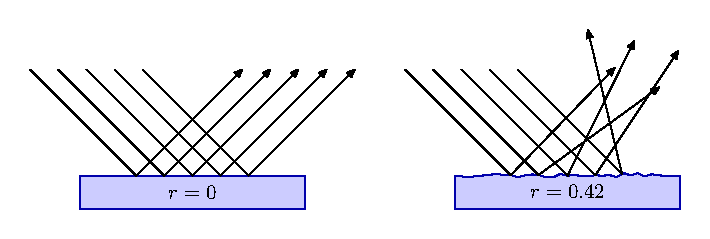
\includegraphics[width=0.95\textwidth]{random-qed}$$
These diagrams are supposed to represent light rays reflecting from a surface: on
the left the surface is smooth ($r=0$) and on the right it's rough ($r=0.42$).
The parameter $r$ is used in the \MP\ program as a scaling factor for the random
noise added to each point along the rough surface; the only difference in the code
to produce the two figures was the value of $r$.%
First the base block is created with some noise on the upper side.  Then five rays
are created.  Applying \mpl{ypart} to the pair of times returned by
\mpl{intersectiontimes} gives us the point of the base where the incident ray hits
it.  This point and the perpendicular at that point are then used to get the angle
for the reflected ray.  The diagrams are effective because the rays are reflected at
realistic looking angles.

The simple approach to adding noise along a path works well in most cases provided
there's not too much noise,  but it is always possible that you'll get two consecutive
values at opposite extremes that will show up as an obtrusive jag in your line.  To
fix this you can simply run your program again to use a different random seed value;
or you could try using ".." instead of "--" to connect each point, but beware that
sometimes this can create unexpected loops.

\newpage\subsubsection{Walking along a torn edge}

It's also possible to use a random
walk approach so that each random step takes account of the previous one to avoid
any big jumps.  Here's one way to do that.
$$
\includegraphics{random-torn-straight-edge}$$
\mpexternal[firstline=6,lastline=12]{random-torn-straight-edge.mp}

\noindent
The "walkr" routine works like the "incr" and "decr" commands; it updates the value of the
argument.  The idea is that the further away from zero you are, the more likely is
that the next value will take you back towards zero.
\mpexternal{random-torn-edge.mp}
You can use this to produce more realistic torn edges.  You can also apply this as a
form of jitter to a curved path, by adding a suitably rotated vector to enough
points along the path, as shown in the example on the right.\rightarrowfill

\moveright5.5in\vbox to 0pt{\kern-4in
\mpexternal[firstline=6,lastline=16]{random-torn-edge-circle.mp}
$$
\includegraphics{random-torn-edge-circle}$$
\vss}


\newpage
\section{Plane geometry}

\noindent\vadjust{\moveright5.5in\vbox to 0pt{\hsize4in\kern-9pt\noindent
Here is the equilateral triangle point macro in action.
$$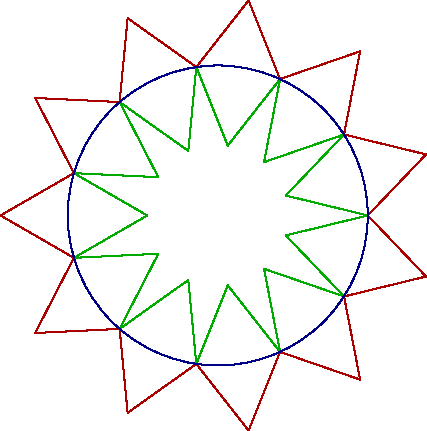
\includegraphics{geometry-triangles-on-circle}$$
\vskip -12pt
\mpexternal[firstline=8,lastline=21,xleftmargin=0pt]{geometry-triangles-on-circle.mp}
\vss}}%
This section deals with drawing geometrical figures that involve lines,
angles, polygons, and circles.  Plain \MP\ provides very few tools that are
explicitly designed to help draw geometric figures, but it is usually possible to
find an elegant construction using these tools and the relevant primitive commands.
It is tempting to build up your own library of special purpose macros, but
experience suggests that it is often better to adapt a general technique to the task
in hand, and to create a specific solution to your current problem.  One of the main
issues is catching exceptions; since it is hard to write completely general macros,
I have tried simply to present each technique so that you can understand it and adapt
it as required.

The classical constructions from Euclid's \textsl{Elements} are often useful
sources of inspiration for macros, but they do not always point in the right
direction.  For example consider the first proposition: \textit{given two points
find a third point, so that the three points make an equilateral triangle}.
Euclid's construction is to draw an arc, with radius equal to the length of the
segment between the two points, at each point and find the intersection.  This might
lead us to a function like this:
\begin{code}
vardef equilateral_triangle_point(expr a, b) =
  save c; path c; c = fullcircle scaled 2 abs(b-a);
  (c shifted a intersectionpoint c shifted b)
enddef;
\end{code}
This works but has a couple of issues.  First using \mpl{intersectionpoint} feels a
bit like cheating; secondly, and more seriously, the point returned depends on the
orientation of the points "a" and "b".  In some configurations the first
intersection found will be on the left, in others on the right.  We could fix this
by rotating the circle "c" by "angle (b-a)", but we can do better with a simple
rotation of the second point about the first:
\begin{code}
vardef equilateral_triangle_point(expr a, b) =
  b rotatedabout(a,60)
enddef;
\end{code}
And if you want to get right back to primitives you could even write that as:
\mpexternal[firstline=5,lastline=7]{geometry-triangles-on-circle.mp}


\newpage
\subsection{Bisecting lines and paths}

\moveright5.5in\vbox to 0pt{\hsize4in\noindent
$$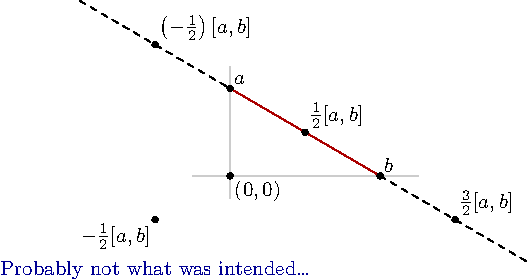
\includegraphics{geometry-mediation-pitfall}$$
\vskip 50pt
$$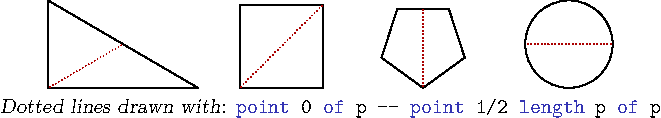
\includegraphics[width=4in]{geometry-mediation-shapes}$$
\bigskip
$$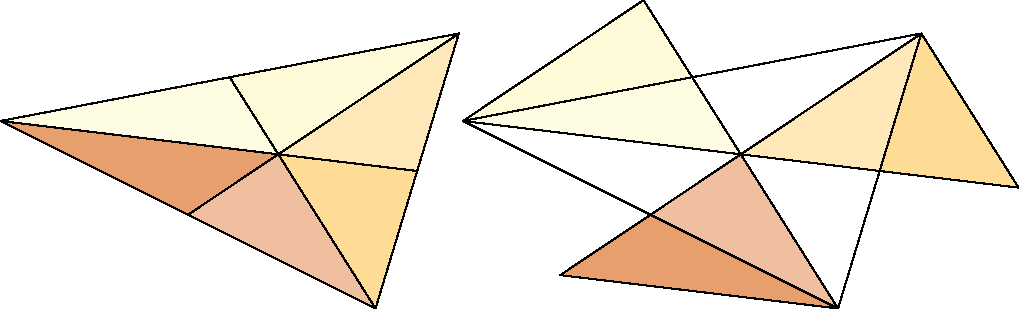
\includegraphics[width=4in]{geometry-mediation-sallows}$$
\centerline{\textsl{Lee Sallows' theorem of median triangles}}
\vss}
\noindent
\textsc{The best way to bisect} a line depends on how you have defined it.
If you have two \<pair>s $a$ and $b$, then the simplest way to find
the \<pair> that bisects them is to write "1/2[a,b]".  This mediation
mechanism is entirely general, so you can write "1/3[a,b]", "1/4[a,b]", and
so on to define other pairs that are part of the way from $a$ to $b$.
But the number before the left bracket does not have to
be confined to the range $(0,1)$.  If you write "3/2[a,b]" you will get a pair on
the extension of the line from $a$ to $b$ beyond $b$.  To get a pair going the
other way you can either reverse $a$ and $b$, or use a negative number; but don't
get caught out by the \MP\ precedence rules:  "-1/2[a,b]" is interpreted as
"-(1/2[a,b])" and not as "(-1/2)[a,b]", so either put in the parentheses or swap
the order of the pairs: "(3/2)[b,a]". See \rightarrowfill

If you want to work with a \<path> variable, rather than separate \<pair>
variables, you can
use the \mpl{point t of p}
notation to do mediation along the path.  For a simple straight path $p$ of length 1
then \mpl{point 1/2 of p} will give you the midpoint.  More generally,
\mpl{point 1/2 length p of p} will give you the midpoint of a path of any length.
This works fine for simple paths, along which \MP's time moves evenly,
but for more complicated, curved paths you have to use this rather cumbersome notation:
\begin{code}
    point arctime 1/2 arclength p of p of p
\end{code}
If your path makes a regular polygon, then you can bisect the shape with the line
\begin{code}
    point t of p -- point t + 1/2 length p of p
\end{code}
\noindent
\hey If the polygon has an odd number of sides, then $2t$ must be a whole number.

\vfill\noindent
\textsc{In a triangle} these bisecting lines are called medians.  The three medians intersect
at the centroid of the triangle.  The centroid is a good place to put a label on a
triangle.  You could find it using the macro from \ref{polygons}, or with
a construction using \mpl{whatever} on any two medians, but since we know that the centroid
divides each median in the ratio $2:1$ we can find the centroid of a triangle path
$p$ most simply with:
\begin{code}
    z0 = 2/3[point 0 of p, point 3/2 of p];
\end{code}
The median lines are the basis for several beautiful theorems about the geometry of the
triangle. The theorem shown here was first published in 2014.

\newpage
\subsection{Bisecting angles}\label{sec:bisect}
\moveright5.5in\vbox to 0pt{\hsize4in\noindent
$$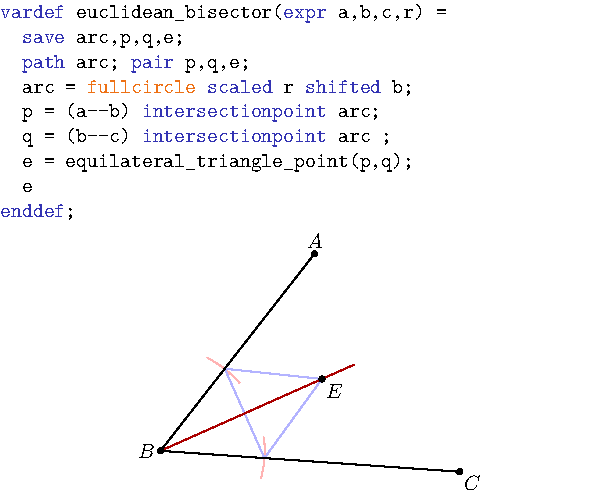
\includegraphics{geometry-bisection-euclidean}$$
\smallskip
$$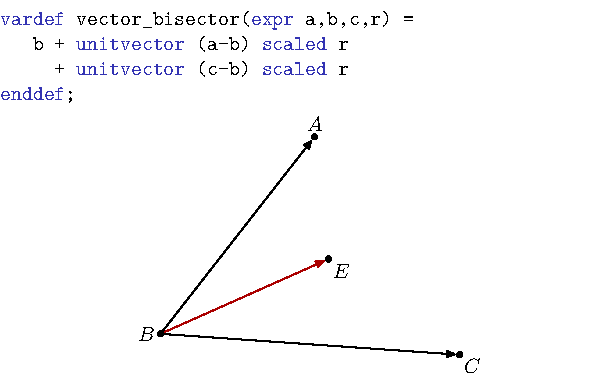
\includegraphics{geometry-bisection-vector}$$
\vss}
\noindent
In an equilateral triangle the medians also bisect the angles at each vertex; this
is the basis of Euclid's method of bisecting an angle set out in the Second
Proposition.  You can do the same in \MP, but it might not always be the best way.
Whatever approach you take, an angle is defined by three points; one that defines
the corner and two that define the lines extending from that corner.  In this
exploration I've used $a$, $b$, and $c$ to represent the points, with $b$ being the
one in the middle, and at the corner.

Euclid's method is to draw an arc centred at the corner, and then construct an
equilateral triangle on the two points where the arc crosses the lines. This is
shown on the right, with a macro that re-uses the equilateral triangle point macro
given above.  But if your aim were to find any point on the line bisecting $\angle
ABC$, then you could simplify this and make it more efficient by using
$e = \frac12[p,q]$
instead of calling the triangle macro at all.  However the macro is still making two
calls to \mpl{intersectionpoint}.  If you wanted to eliminate this you could use the
useful plain \MP\ macro \mpl{unitvector} to produce a solution based on adding two equal
length vectors from the corner to the two other points.  Another approach is to
exploit another geometric theorem that states that the bisector of an angle in a
triangle divides the opposite side in the ratio of the two other sides.
So if sides $AB$ and $BC$ have lengths $p$ and $q$ then the bisector will
be ${p\over p+q}={1\over1+q/p}$ from $A$ to $C$, and you can express this
simply using \MP's mediation syntax:
\vbox to 0pt{
$$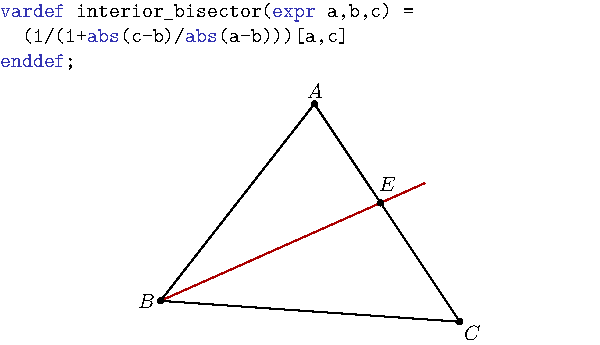
\includegraphics{geometry-bisection-interior}$$
\vss}

\newpage
\subsection{Trisections and general sections of angles}

There is no classical method to trisect an arbitrary angle, so you need to resort
to measuring and arithmetic in \MP.  If the angle is a given this is trivial:
\mpic{-12pt}{geometry-trisection-simple}
\smallmpexternal[firstline=6,lastline=17]{geometry-trisection-simple.mp} 

\noindent
But if you have only the coordinates of some points then you need to use the
\mpl{angle} primitive to measure the angle first; \mpl{angle} takes a \<pair>
argument and returns a numeric representing the angle in degrees measured clockwise
from the $x$-axis to a line through the origin and the point represented by the pair.
This definition means that if you have three points $A$, $B$, and $C$, then you can
measure $\angle ABC$ with \mpl{angle(C-B)-angle(A-B)}. Following the usual
convention this gives you the angle at $B$; if you list the points in clockwise
order you will get a positive result. If you don't care about the order, you
can make this into a more robust macro:
\begin{smallcode}
vardef measured_angle(expr P, Q, R) =
  (angle (P-Q) - angle (R-Q)) * turningnumber (P--Q--R--cycle) mod 360
enddef;
\end{smallcode}
The primitive \mpl{turningnumber} is explained on p.\thinspace 111 of \textsl{The
METAFONTbook}.  It takes a closed path and returns number of times that you would
turn through 360${}^\circ$ if you traversed the path.  We use this here to
negate the measured angle if necessary, so that you always get the interior angle.
The \mpl{mod 360} on the end ensures that the result is in the range $0 \le \theta <
360$.  Armed with a measured angle, all you then need is arithmetic.
\mpic{-160pt}{geometry-trisection-classical}
It might be possible to use the \id{solve} macro to simulate the Neusis construction
(that allows you to measure a length) illustrated on the right, but measuring the
angles is rather easier.

\newpage
\subsection{Intersections}\label{sec:intersect}

\moveright5.5in\vbox to 0pt{\hsize4in\noindent
\centerline{A puzzle square featuring some intersections}
$$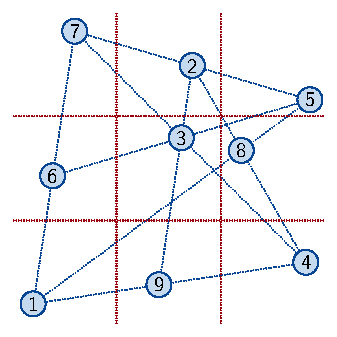
\includegraphics[width=3in]{geometry-magic-square-14}$$
The points were defined like this (the order was important).
\mpexternal[firstline=8,lastline=18]{geometry-magic-square-14.mp}
\vss}
\noindent
If you have line segments defined by their endpoints, then the
canonical way to find their intersection, is to use
the mediation syntax with \id{whatever} twice:
$$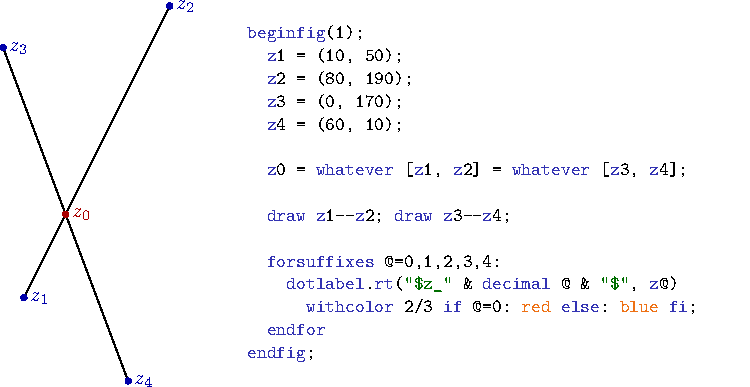
\includegraphics{geometry-whatever}$$
The mediation syntax works even if the intersection point does not actually lie on
either of the two line segments.  The intersection will be the point where the two
(infinite) lines through the pairs of points meet.  If the two lines are parallel,
you'll get an `inconsistent equation' error.  If you want to capture the calculated
values, then use undefined numeric variables instead of \id{whatever}:
\begin{code}
    z0 = alpha [z1, z2] = beta [z3, z4];
\end{code}
In this example you would find $\alpha=0.286$ and $\beta=0.5$.
If you are trying to find where the line through your points intersects a horizontal or vertical, then you only need one
mediation and a simple equation for the relevant $x$ or $y$ coordinate:
\begin{code}
    z0 = alpha [z1, z2]; x0 = 0;  % for example
\end{code}
If you have defined your lines as paths, and especially if they are more complicated
than straight lines, you need to use the \mpl{intersectiontimes} primitive or the
\mpl{intersectionpoint} macro, as explained on pp.136–137 of \mfbook.

\newpage
\subsubsection{The intersection algorithm}

\MP\ inherits a fast algorithm for finding the intersection between two paths from
\MF.  It is explained rather more gnomically than usual at the end of Chapter 14 of
\mfbook, with more detail given in the web source for \MF.  The core algorithm works
on paths of length 1. If you have longer paths, \MP\ works its way along the paths
applying the core algorithm to successive pairs of unit subpaths.  It does this is
lexicographic order; this means that, if you have two circles $A$ and $B$, and you do this:
\begin{code}
    (t, u) = A intersectiontimes B;
\end{code}
then \MP\ will first look for an intersection between subpath $(0,1)$ of $A$ and
subpath $(0,1)$ of $B$, then subpath $(0,1)$ of $A$ and subpath $(1,2)$ of $B$, and
so on, with $B$ varying faster, until you get to subpath $(7,8)$ of $A$ and subpath
$(7,8)$ of $B$.  But you may never get that far, as the process stops as soon as the
first intersection is found.  The upshot of this is that the intersection point
found will always be as early as possible on $A$.  Note that after the call above
point $t$ of $A$ will be very close to point $u$ of $B$, as they both refer to the
same intersection point.  If you want the alternative point that is earlier on $B$,
then use `$B \mathbin{\textrm{intersectiontimes}} A$'
instead.\mpic{-222pt}{geometry-intersection-AB-or-BA}

\vfill\noindent
When we get down to paths of length 1, the algorithm works something like this:

$$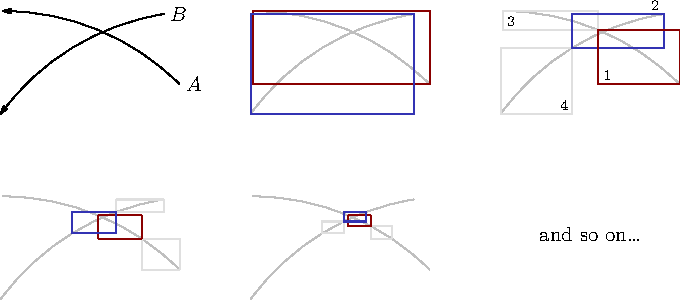
\includegraphics{geometry-intersection-algorithm}$$
\vadjust{\moveright 384pt\vbox to 0pt{\hsize 4.2in\vss \noindent
The two paths are represented as rectangles that enclose the end points and the
control points for each path.  If these rectangles don't overlap then there is
certainly no intersection. Otherwise \MP\ bisects each path and considers four
smaller rectangles, in the order $(1,2)$, $(1,4)$, $(3,2)$, $(3,4)$ (as shown).  In
this case it will pick $(1,2)$, discard 4, and push 3 onto a stack.  It carries on
doing this, back tracking as required, until it finds sufficiently small overlapping
rectangles.  The two times returned by \mpl{intersectiontimes} are the midpoints of
the subpaths enclosed by these two tiny rectangles, which is why they do not always
refer to exactly the same point.}}

\subsubsection{Finding all intersection points}\label{sec:allxp}

As noted above, the \mpl{intersectiontimes} algorithm will stop at the first
intersection of the two paths, but it is possible that the two paths will intersect
again further along.  If you want to find all the intersection points then the
simplest technique is just to unwrap the algorithm slightly, and loop through all
the unit subpaths applying \mpl{intersectiontimes} to each pair.  Using an array to
hold the points and a counter, you can get them with something like this:
\begin{smallcode}
pair P[], times; numeric n; n = 0;
for i = 1 upto length(A):
  for j = 1 upto length(B):
    times := subpath (i-1,i) of A intersectiontimes subpath (j-1,j) of B;
    if xpart times > -1:
      P[incr n] = 1/2[point xpart times of subpath (i-1,i) of A,
                      point ypart times of subpath (j-1,j) of B];
    fi
  endfor
endfor
\end{smallcode}
and then use them like this:
\begin{smallcode}
for i=1 upto n:
    draw fullcircle scaled 4 shifted P[i]; % or whatever
endfor
\end{smallcode}
There are a couple of \MP\ technical points to note.  The \mpl{intersectiontimes}
operation returns a pair, which we assign to a pair variable $\id{times}$
above; we have to use \mpl{:=} to re-assign it in each loop, and we have to
use an explicit pair variable because you can't assign to a literal pair;
\MP\ will give you an error if you try \mpl{(t, u) := A intersectiontimes B;}.
This may come as a surprise, because you \textit{can} legally do \mpl{(t, u) = A
intersectiontimes B}, but in a loop this causes an inconsistent equation error on
the second iteration.  If you need to avoid the repeated use of \mpl{xpart} and
\mpl{ypart}, one alternative is to do this inside the loop:
\begin{smallcode}
...
numeric t, u;
(t, u) = A intersectiontimes B;
...
\end{smallcode}
Now the numerics are reset each time and the equation is not inconsistent.
\vadjust{\moveright 384pt\vbox to 0pt{\hsize 4.2in\vss \noindent
T\textsc{he} technique discussed on the left, works well on paths where the points on one or
both of the paths are close together, so that the unit subpaths are short;
But it
is possible to create quite long paths of unit \mpl{length} and these may intersect
each other more than once, like so:
$$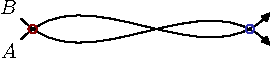
\includegraphics{geometry-intersection-only-two}$$
Here the two paths $A$ and $B$ are Bézier splines of with \mpl{length=1}, so the
normal \MP\ algorithm is only ever going to give you one of the intersections.  In
the diagram above, the
red circle marks the point given by \mpl{A intersectiontimes B}.  We can try
reversing the first path, and in this case you get the point marked in blue,
but what about the one in the middle?

The most reliable approach is to take a copy of one of the paths, and snip it off at
the intersection and try again until there is nothing left to snip.
$$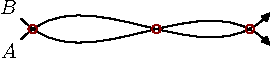
\includegraphics{geometry-intersection-all-three}$$
The three points marked here were captured like this:
\mpexternal[firstline=13,lastline=20]{geometry-intersection-all-three.mp}
\noindent
This technique also works on paths with \mpl{length} greater than one,
so you may prefer it as your general “get all the intersections” approach.
Note that the \mpl{cutbefore} macro is defined using \mpl{intersectiontimes}.

\kern 6.5pt
}}


\subsection{Parallel and orthogonal or whatever}\label{sec:parallel}

Given five known points --- $A$, $B$, $C$, $D$, and $E$ --- \MP\ can find the point $F$
on the line $A \to B$, so that $E \to F$ is parallel to $C \to D$ like this:
\mpic{0pt}{geometry-parallel}
\begin{code}
    F = whatever[A, B]; % F is on the line A..B
    E-F = whatever * (C-D) % E..F || C..D
\end{code}
In the second line the expressions \mpl{E-F} and \mpl{C-D} return \<pair>
variables and the equation with \mpl{whatever} says that they must be scalar
multiples of each other.  With the first equation, this is enough for \MP\ to work
out where $F$ should go.   Note that \mpl{whatever} can take any real value,
positive or negative, so it does not matter whether you put \mpl{E-F} or \mpl{F-E}.
Note also that for the same reason, while $F$ will lie on the \textit{line} through
$A$ and $B$, it might not lie on the \textit{segment} from $A$ to $B$.
But also note that you \textit{cannot} write the second equation as
\begin{code}
    E-F * whatever = (C-D); % <--- gives an error
\end{code}
because you can only apply \mpl{whatever} to known quantities.

\bigskip\noindent\llap{\nb}%
To define a line perpendicular to $C\to D$ rather than parallel, then you can write:
\begin{code}
    G = whatever[A, B];
    E-G = whatever * (C-D) rotated 90;
\end{code}
and obviously the "90" can be adjusted to whatever angle you please, if you want
something between parallel and orthogonal.

\smallskip\noindent\llap{\nb}%
To define the line through $E$ that is perpendicular to $A\to B$, you should just
use $(A-B)$ instead of $(C-D)$.  The diagram shows $H$, the point on $A\to B$
that is closest to $E$; you can (I trust) work out how to define that yourself.

\smallskip\noindent\llap{\nb}%
If you just need to compute the perpendicular distance from the point $E$ to a line $A\to
B$, rather than defining the point $H$, then you can use Knuth's ‘slick’ formula:
\begin{code}
    abs ypart ((E-A) rotated -angle (B-A))
\end{code}
This effectively rotates $E$ about $A$ by the angle of the line, so that the problem
is reduced to measuring the height of a point above the $x$-axis, which is what
\mpl{ypart} does, of course.

\moveright5.5in\vbox to 0pt{\hsize 4in\vss\noindent
There are some limitations to what you can do with \MP's linear equations; for one
thing you can't generally say things like \mpl{length(C-A) = 72}.  If you want to
find the two points on a line that are a given distance from an external point, it's
often simpler to find the intersection points of the line with a suitably scaled and
shifted circle, even if you don't actually then draw the circle.  You can usually
find the other point by reversing the circle.\par}

\newpage
\subsection{Drawing circles}\label{sec:circles}

The canonical way to draw a circle in plain \MP\ is to use the pre-defined path
\mpl{fullcircle} with a suitable transformation.
\mpic{-12pt}{geometry-drawing-circles}
The path is defined (in "plain.mp") using two \MP\ primitive commands:
\begin{code}
path fullcircle; fullcircle = makepath pencircle;
\end{code}
A \kw{pencircle} is the basic nib that is used to draw lines that digitize neatly;
it represents a true circle of diameter 1, passing through the points $(\pm.5, 0)$
and $(0, \pm.5)$.  When processed with \kw{makepath} it turns into a closed
polygonal path with eight points that closely approximates a circle with diameter
1\unit{bp} centred on the point $(0, 0)$.  To use it, you can scale it and shift it.
To draw a circle with radius 2\unit{cm} at the point $(34, 21)$ you would do:
\begin{code}
draw fullcircle scaled 4cm shifted (34, 21);
\end{code}
Remember to scale before you shift, and that \id{fullcircle} has unit
\textit{diameter}, not unit \textit{radius}.  To draw a circle centred at point $A$
that passes through point $B$ [\red{I}] try:
\begin{code}
draw fullcircle scaled 2 abs (B-A) shifted A;
\end{code}
There are of course an infinite number of circles that you can draw through two
points, but if the line between the two points is a diameter [\blue{II}], then you can do:
\begin{code}
draw fullcircle scaled abs (B-A) shifted 1/2[A,B];
\end{code}
Finally three points define a unique circle [\green{III}]:
\mpexternal[firstline=27,lastline=32]{geometry-drawing-circles.mp}
\noindent
Plain \MP\ also defines \id{halfcircle} and \id{quartercircle}, as the appropriate
subpaths of \id{fullcircle}, both starting at point 0 (3 o'clock). Curiously, this
differs from \MF\ where \id{quartercircle} is defined first, and the other two
composed from it. The reference point of these two paths is the center of the
complete circle of which they would be part; so if you did “\kw{draw}
\id{quartercircle} \kw{shifted} $(34, 21)$;”, you would get an quarter-circle arc from
$(34.5,21)$ to $(34,21.5)$.

\newpage
\subsection{Incircle and excircle of a triangle}

The incircle of a triangle is the largest circle contained in the triangle.
The centre of the incircle lies at the intersection of the internal angle bisectors.
So we can use ideas from §\ref{sec:bisect} and §\ref{sec:intersect} to define a
macro that returns the required path given points $A$, $B$, and $C$:
\mxpic{-1in}{5in}{geometry-incircle}
\mpexternal[firstline=11,lastline=18]{geometry-incircle.mp}

\bigskip\noindent
The excircles of a triangle are the three circles lying outside the triangle and
tangent to one edge and the extensions of the other two.  The centres of each
excircle lie at the intersection of one internal angle bisector and the external
angle bisector of one of the other corners.

To get the external angle bisector,
all you have to do is reverse the direction of one of the \mpl{unitvector} calls 
(can you see why?)
\mxpic{0pt}{5in}{geometry-excircle}
\begin{code}
vardef excircle(expr A,B,C) =
  save a, b, m, t; pair a, b, m, t;
  a = A + unitvector (C-A) - unitvector (B-A);
  b = B + unitvector (A-B) + unitvector (C-B);
  m = whatever[A,a] = whatever [B,b]; t = whatever[A,B];
  t-m = whatever * (B-A) rotated 90;
  fullcircle scaled 2 abs (t-m) shifted m
enddef;
\end{code}

\smallskip\noindent
To get the other excircles, call the macro with the points in a different order.

\newpage
\subsection{Circumcircle of a triangle}

The circumcircle of a triangle is the circle through the three corners, so if you
already have the corners of your triangle as separate \<pair> variables, you can
use the \mpl{circle_through} macro from §\ref{sec:circles}.  Or you can adapt the
macro to take a single triangular path:
\smallmpexternal[firstline=11,lastline=16,xleftmargin=0pt, xrightmargin=-60pt]{geometry-circumcircle.mp}
\noindent
Note that as the diagram on the right shows,\mxpic{-2in}{4.6in}{geometry-circumcircle}
the centre of the circumcircle is the intersection of all three of the perpendicular bisectors of
sides, but for the purposes of drawing in \MP\ you only need to find the
intersection of two of them.  You could write 
\begin{smallcode}[xleftmargin=0pt, xrightmargin=-60pt]
  m = whatever * (point 0 of T - point 1 of T) rotated 90 shifted point 1/2 of T 
    = whatever * (point 1 of T - point 2 of T) rotated 90 shifted point 3/2 of T 
    = whatever * (point 2 of T - point 3 of T) rotated 90 shifted point 5/2 of T; 
\end{smallcode}
but this does not add any more information to the equation for $m$, and
\MP\ will sometimes give you an “inconsistent equation” error if your triangle 
is long and thin.

\vfill
\noindent
\hey The marks that show line segments are equal were created by this macro.
\smallmpexternal[firstline=38,lastline=47]{geometry-circumcircle.mp}
Given the triangular \<path> $T$, the macro was used like this: 
$\longrightarrow$\vadjust{\moveright5.5in\vbox to 0pt{\vss
\smallmpexternal[firstline=49,lastline=51]{geometry-circumcircle.mp}
}}

\newpage
\subsection{The nine-point circle of a triangle}

The orthocentre of a triangle is the point at the intersection of the three
altitudes, shown as point $D$ below.
The point $N$, half-way from $D$ to the
circumcentre $M$ is the centre of the remarkable nine-point circle which passes
through the bases of the three altitudes and bisects the six line segments $AB$, $AC$, $AD$,
$BC$, $BD$, and $CD$.\vadjust{\moveright5.25in\vbox to 0pt{\hsize 4in\vskip-88pt\noindent
\smallmpexternal[firstline=6,lastline=52,xleftmargin=0pt]{geometry-nine-point-circle.mp}
\vss}}

\smallskip

$$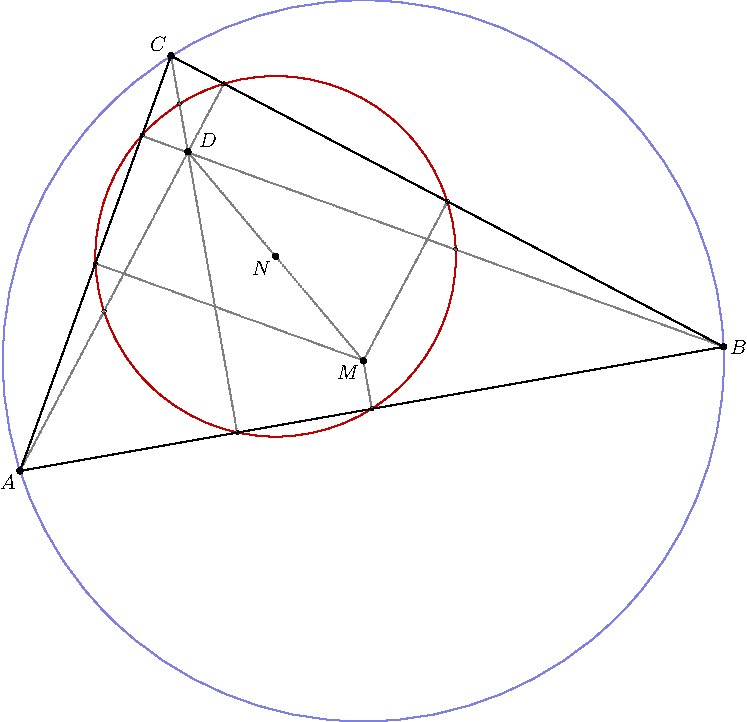
\includegraphics{geometry-nine-point-circle}$$

\newpage
\subsection{Lines tangent to a point on a path}

\MP\ represents paths internally as a sequence of nodes. Each node consists of three
pairs: the pre-control point, the point itself, and the post-control point. 
\mpic{0pt}{geometry-tangents-on-path}%
For a given path $p$ you can extract these points at time $t$ with these operators:
\begin{code}
precontrol t of p
point t of p
postcontrol t of p
\end{code}
Unless you explicitly set them differently, \MP’s curve fitting will make these
three points co-linear, so you can draw a tangent at point $t$ with 
\begin{code}
draw precontrol t of p -- postcontrol t of p;
\end{code}
The length of the tangent line drawn
like this depends on the size and shape of the curve, but it is somewhat arbitrary.
So you may prefer to extract a \<pair> representing the tangent at point $t$ with
\begin{code}
pair d; d = postcontrol t of p - precontrol t of p;  
\end{code}
In fact, this is so useful that
"plain.mp" provides \mpl{direction} as a shorthand:
\begin{smallcode}[xleftmargin=0pt, xrightmargin=-20pt]
vardef direction expr t of p = postcontrol t of p - precontrol t of p enddef;
\end{smallcode}
which can save you some typing.  But the clever bit is that $t$ does not have to be a whole
number.  If you set $t=\frac14$ (say), \MP\ works out the corresponding fractional
control points, so that you can use \mpl{direction t of p} to get a tangent at any point.  

The vector pairs returned have the right direction, but still have rather arbitrary magnitudes, so
the usual idiom is something like this:
\begin{smallcode}
path s; s = origin -- 36 unitvector(direction t of p);
drawarrow s shifted point t of p;
\end{smallcode}
or the snippet shown on the right $\longrightarrow$

\newpage
\subsection{Lines tangent to a circle}\label{sec:tangent-times}

The techniques of the preceding section can be used to add a tangent line to a
given point on a circular path, but not to find the tangent lines from a given point
outside a circle.  To do this, you need to adapt the standard geometrical
construction: for a given circle $C$ and a point $p$, find the midpoint of $p$ and
the center of $C$; draw a semicircle through $p$, centred on this midpoint; the tangent
point is where the semicircle intersects $C$. %
\mpic{-110pt}{geometry-tangents-point-to-circle}
Given a suitable \mpl{path C} and \mpl{pair p} you can do this:
\mpexternal[firstline=11,lastline=13]{geometry-tangents-point-to-circle.mp}

\noindent
No parentheses are needed around the second path, because \mpl{intersectionpoint} is
defined with \mpl{secondarydef}.

\medskip\noindent
Things are a little more complicated if you want the points as times along the path
$C$ and you care about which tangent point is which.  Here is a routine that returns
the tangent points from $p$ as two times $a$ and $b$ on $C$, with $b$ adjusted so
that $b > a$ in all cases regardless of the relative rotation of $C$ and $p$.  This
means that \mpl{subpath (a, b) of C} is always the “long way round” C, on the
opposite side from $p$, and \mpl{subpath (a, b-8) of C} is always the shorter
segment.

\mpexternal{geometry-tangent-times.mp}

\noindent
Note the elegant syntax here; if \mpl{z} is a \<pair> then the operation
\mpl{zscaled z} is equivalent to \mpl{scaled abs z rotated angle z}.

\vpic{-200pt\noindent Here is the macro in action.
Having obtained the two times $a$ and $b$ from the macro, the dashed line
was drawn along a path that was composed with:
\vrule depth 20pt width 0pt height 2pt
\mpl{p -- subpath (a,b) of C -- cycle}
}{geometry-tangent-times-on-circle}

\newpage
\subsection{Lines tangent to two circles (exterior)}\label{sec:adjust-times}

The same \mpl{tangent_times} macro can be reused to find the tangents that touch two
circles, using an approach like this: \mwpic{-36pt}{geometry-tangents-two-circles-exterior}

\smallmpexternal[firstline=9,lastline=24]{geometry-tangents-two-circles-exterior.mp}

Here $A$ and $B$ are the two circles you want to connect, and $A$ is larger than
$B$. $R$ is the radius of the larger, $r$ of the smaller. $C$ is an auxiliary circle
centred at the same point as $A$ and scaled so that its radius is $R-r$.  If we
then find the tangent points on $C$ from the center of $B$, the points we want are
the corresponding points on $A$ and $B$. 

Notice how the times are used with \mpl{subpath}; if $a>b$, then the path returned
from \mpl{subpath (a, b) of P} is the same as \mpl{reverse subpath (b, a) of P},
which means that \mpl{subpath (u,t) of B} would give you the wrong side.  The remedy
is to substract 8 from $u$ (or, more generally, to subtract the length of path $B$).
Because there are 8 points on a \mpl{fullcircle} path, point $u$ and point $u-8$
refer to the same place, but since $u-8 < t$, the subpath will run clockwise as
required.  

\vfill
\noindent\hey
This all works provided that all three 
circles $A$, $B$, or $C$ have the same rotation. 
But this may not always be the case.   
For example, you might have defined $B$ as 
\begin{code}
B = fullcircle scaled 60 shifted 240 dir 36;
\end{code}
and then point $t$ of $B$ would \textit{not} correspond to point $t$ of the
auxiliary circle $C$.  
\vadjust{\moveright5.5in\vbox to 0pt{\hsize 4in\vss\noindent
To cope with circles that might not have the same rotation, you need to adjust the
tangent times to take account of the different relative rotation.
\mpexternal[firstline=7,lastline=10]{geometry-tangents-two-circles-interior.mp}
\noindent
This macro exploits the relationship between \mpl{angle}
and points around a \mpl{fullcircle} path:  $360^\circ = 8\:\hbox{points}$.
You can see it in action on the followin page.
}}

\newpage
\subsection{Lines tangent to two circles (interior)}

To find the interior tangents, you just need to add the smaller radius rather than
subtract it, and add 4 to the times on the smaller circles, so that they are on the
other side:
$$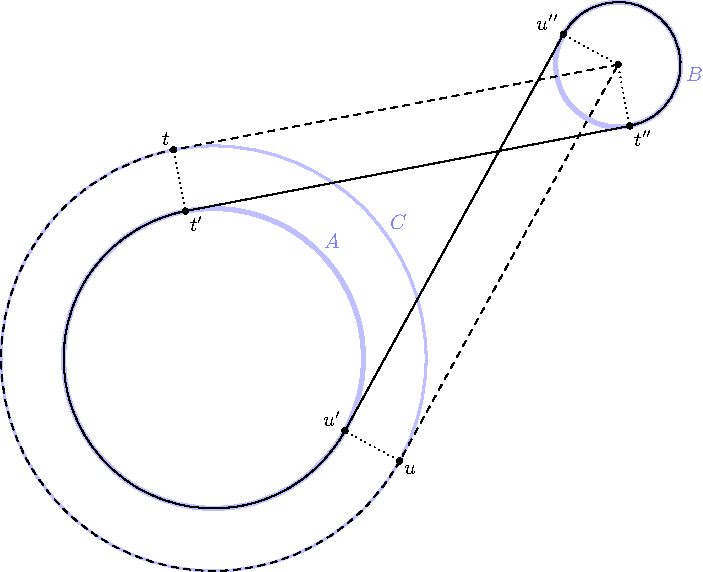
\includegraphics[width=\textwidth]{geometry-tangents-two-circles-interior}$$

\bigskip\noindent
The complete code for this is shown on the right.  It uses the same
routines given above; \mpl{tangent_times} from section \ref{sec:tangent-times}, and
\mpl{adjust_time} from section \ref{sec:adjust-times}.
\vadjust{\moveright5.25in\vbox to 0pt{\hsize 4in\vss\noindent
\smallmpexternal[firstline=12,lastline=54]{geometry-tangents-two-circles-interior.mp}
\vskip -72pt
}}

\subsection{Axis of similitude}\label{sec:axosim}

\vbox to 0pt{\vskip-\baselineskip\noindent\hbox to
\textwidth{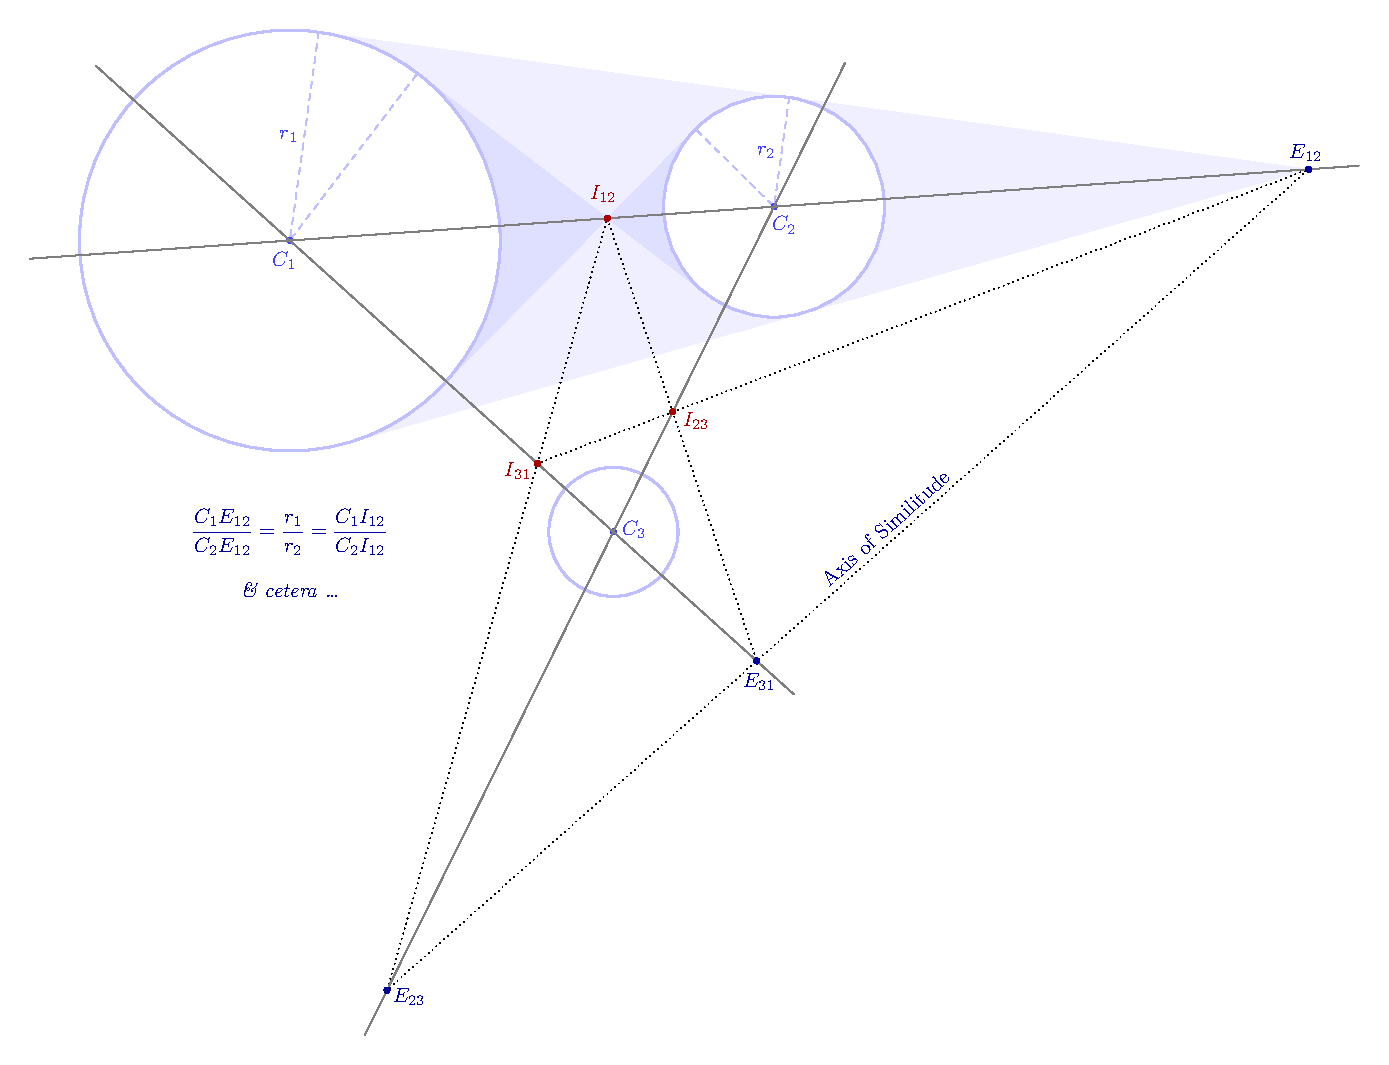
\includegraphics[scale=0.92]{geometry-axis-of-similitude}\hss}\vss}

\vfill
\moveright5.5in\vbox to 0pt{\hsize 4in\vss\noindent
Given three circles taken in pairs, you can use the techniques of the preceding
sections to find the three points where the common external tangents
intersect (shown here as $E_{12}$, $E_{31}$, and $E_{23}$) and the
three points where the common internal tangents intersect ($I_{12}$,
$I_{31}$, and $I_{23}$).  These points have a pleasing collinearity.
The line common to the three $E$ points is known as the \textit{Axis of
Similitude}.

The drawing is left as an exercise for the reader, except
to note that if \mpl{r1} and \mpl{r2} are \<numeric> variables representing
the radius of the circles centred at the \<pair> variables \mpl{C1} and \mpl{C2},
then:
\begin{smallcode}
E12 = (r1/(r1 - r2)[C1, C2]; I12 = (r1/(r1 + r2)[C1, C2];
\end{smallcode}
which is a bit quicker than working out all the tangent points. 
My version is in the file "geometry-axis-of-similitude.mp"
}

\newpage
\subsection{Inversion, pole, and polar}\label{sec:inversion}

Inversion in a circle is a generalization of reflection in a line.
\mpic{-48pt}{geometry-pole-and-polar}
It is useful for certain constructions in geometry, and easy to implement as a macro
\MP.  For given circle, and a given point $P$ lying outside the circle, the inverted
point $P'$ lies inside the circle at the intersection of the line from $P$ to the
centre of the circle, and the line between the tangent points
[§\ref{sec:tangent-times}] from $P$, shown here as $Q$ and $R$.\rlap{\quad$\longrightarrow$}

But $OPQ$ and $OQP'$ are similar triangles, so $r/OP=OP'/r$ and so $OP' =
r^2/OP$, and since $P'$ must lie on the line through $O$ and $P$, this is enough to
to find $P'$ directly given $P$, $O$, and $r$:
\begin{code}
P' = O + unitvector(P-O) scaled (r * r / abs (P-O));
\end{code}
But examining "plain.mp" shows that \mpl{unitvector} is a macro defined like this:
\begin{code}
vardef unitvector primary z = z/abs z enddef;
\end{code}
which suggests this alternative formulation:
\begin{code}
P' = O + (P - O) scaled (r / abs (P - O) * r / abs (P - O));
\end{code}
or as a macro, and dividing first to avoid overflow:
\begin{code}
vardef invert(expr P, O, r) = 
  save s; numeric s; s = abs(P - O);
  O + (P - O) / s * r / s * r
enddef;
\end{code}
This works well in most cases, but you could consider checking that $s$ is not too small.
If it is more convenient to deal with the \<path> of the circle of inversion
instead of the centre and the radius, you can get the macro to calculate 
them for you:
\mpexternal[firstline=6,lastline=11]{geometry-pole-and-polar.mp}

\vfill

\moveright5.5in\vbox to 0pt{\vss\hsize 4in\noindent
\noindent\llap{\nb}Inversion is reciprocal, so $P$ is the inverse of $P'$ above. Points
on the circle of inversion invert to themselves.

\smallskip
\noindent\llap{\nb}For any given line, the \blue{\textit{pole}} of
the line with respect to a circle, is the inverse of the point on the line closest
to the centre of the circle.

\smallskip
\noindent\llap{\nb}For any given point, the \blue{\textit{polar}} of
the point with respect to a circle, is the line through the inverse of the point
perpendicular to the line through the point and the center of the circle of
inversion.

\smallskip
\noindent\llap{\nb}The inversion of points on the polar (shown as blue dots)
lie on a circle through $O$ and $P'$.  The complete circle would be the inversion
of the infinitely extended polar.}

\newpage
\subsection{Radical axis and radical centre}\label{sec:radical}

The \textit{radical axis} of two circles is the line, orthogonal to the line between
the centres of the two circles which is the locus of points which have equal power
with respect to both circles; that is the points from which the tangents to each circle
are of equal length.  A circle centred at any point on the axis, and drawn with radius equal to the
length of the tangent will cut both circles at right angles.

\medskip\noindent\centerline{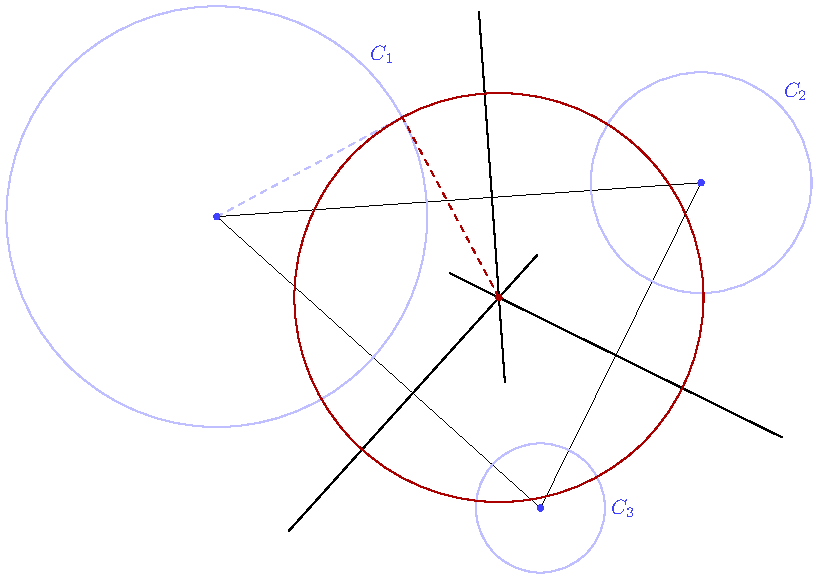
\includegraphics{geometry-radical-axis}}

\medskip\noindent
In a system of three circles as shown, the \textit{radical centre} ("radix") is the
intersection of the three mutual radical axes.  The tangents from this point to all three circles
have the same length, so a circle with this radius (shown above in \red{red})
cuts all three circles at right angles.

\moveright5.5in\vbox to 0pt{\vss\hsize 4in
\smallmpexternal[firstline=6,lastline=51]{geometry-radical-axis.mp}
\vskip -1in}

\newpage
\subsection{Circles tangent to other circles}

\vbox to 0pt{\noindent
\hbox to \textwidth{\includegraphics[height=\textheight]{geometry-apollonius}\hss}
\vss}

\vfill
\moveright5.5in\vbox to 0pt{\hsize 4in\vss\noindent
The classical Problem of Apollonius is to find a circle tangent to three others.
All of the approaches are rather involved, but Gergonne's is probably the simplest
to follow in \MP.

\smallskip\noindent For three given circles \blue{$C_1$, $C_2$, and
$C_3$}, you first find the external \blue{axis of similitude}
[§\ref{sec:axosim}]; then find the \textcolor{carrot}{poles} [§\ref{sec:inversion}] of this line with
respect to each of the three circles; and thirdly find the
\textcolor{squash}{radical centre}
[§\ref{sec:radical}].

\smallskip\noindent
The lines from the radical centre through each of the three
poles cut each circle in two places.  These six points show the tangent points for
the two \red{tangent circles}, and you can draw the circles using the three point circle
technique [§\ref{sec:circles}].

\smallskip\noindent
{\small
The drawing is left as an exercise for the reader, although you can find my
"geometry-apollonius.mp" in the source for this document. You might try to make a more
robust version or to find all the other tangent circles.}}


\newpage
\subsection{Coordinate geometry examples}

\kern-\baselineskip
\vpic{-24pt}{geometry-examples-desargues}

\mpexternal[xleftmargin=0pt,firstline=6,lastline=37]{geometry-examples-desargues.mp}
\moveright 340pt \vbox to 0pt{\vss
\mpexternal[xleftmargin=0pt,xrightmargin=-80pt,firstline=38,lastline=53]{geometry-examples-desargues.mp}
\vskip -42pt}

\newpage
\vpic{-36pt}{geometry-examples-trisections}
\vbox to 0pt{
    \mpexternal[xleftmargin=0pt,xrightmargin=-80pt,firstline=6,lastline=40]{geometry-examples-trisections.mp}
\vss}
\newpage
\kern-3\baselineskip
\vpic{0.25in}{geometry-examples-napoleon}
\vbox to 0pt{
    \mpexternal[xleftmargin=0pt,firstline=6,lastline=37]{geometry-examples-napoleon.mp}
\vss}
\newpage
\kern-3\baselineskip
\vpic{1in}{geometry-examples-projections}
\vbox to 0pt{
    \mpexternal[xleftmargin=0pt,firstline=6,lastline=41]{geometry-examples-projections.mp}
\vss}

\newpage
\moveright5.25in\vbox to 0pt{\hsize4.25in\noindent
\smallmpexternal[firstline=7,lastline=14,xleftmargin=0pt]{geometry-arbelos.mp}
\centerline{\includegraphics{geometry-arbelos}}
\vfill\noindent
\begingroup
\raggedleft\fontsize{8}{10}\selectfont\textsf{%
One must also recognize that any attempt to illustrate geometry\\
involves a basic fallacy.  For example, a straight line is unbounded\\
and infinitely thin and smooth, while any illustration is unavoidably\\
of finite length, of positive thickness, and rough edged.\\[2pt]
— Benoit Mandelbrot, \textsl{The Fractal Geometry of Nature}}
\par\endgroup
\vss}
\smallmpexternal[firstline=15,lastline=52,xleftmargin=0pt,xrightmargin=-72pt]{geometry-arbelos.mp}

\newpage
\subsection{Drawing angle marks}

\textsc{Observant readers} will have noticed that the occasional angle marks in the
preceding examples are generally drawn using plain \MP\ commands rather than a
macro.  This is partly in order to make the examples self-contained and partly to
show what can be done with the default plain \MP\ format. 

\smallskip\noindent
To mark a right angle at point $a$ on the line $a\to b$ you can do something like
this:
\begin{code}
draw unitsquare scaled 5 rotated angle (b-a) shifted a;
\end{code}
with a suitable pen and a suitable colour.  You \textit{could} write a macro to do
this, but it hardly seems worth the effort.%
\vadjust{\moveright 5.5in\vbox to 0pt{\hsize 4.2in\vskip -108pt\noindent
For example, this is one way to annotate a right-angle triangle:
\begin{code}
pair a, b, c; a = 10 dir 10; b = 160 dir 20; 
c - a = whatever * (b - a rotated 90); ypart c = ypart b;
draw unitsquare scaled 5 rotated angle (b-a) shifted a 
    withcolor 3/4;
draw a--b--c--cycle;
\end{code}
which produces this:
$$\begin{mplibcode}
pair a, b, c; a = 10 dir 10; b = 160 dir 20; 
c - a = whatever * (b - a) rotated 90; ypart c = ypart b;
draw unitsquare scaled 5 rotated angle (b-a) shifted a withcolor 3/4;
draw a--b--c--cycle; 
dotlabel.llft("$a$", a);
dotlabel.rt  ("$b$", b);
dotlabel.ulft("$c$", c);
\end{mplibcode}$$

\bigskip\noindent
Equipped with the macro shown on the left, you could add this:
\begin{code}
    draw angle_mark(a, c, b, 16) withcolor 2/3 red;
\end{code}
to get this:
$$\begin{mplibcode}
pair a, b, c; a = 10 dir 10; b = 160 dir 20; 
c - a = whatever * (b - a) rotated 90; ypart c = ypart b;
vardef angle_mark(expr P, O, Q, r) = 
  fullcircle scaled 2r rotated angle (P - O) 
    shifted O cutafter (O -- Q)
enddef;
draw unitsquare scaled 5 rotated angle (b-a) shifted a withcolor 3/4;
draw angle_mark(a, c, b, 16) withcolor 2/3 red;
draw a--b--c--cycle;
    dotlabel.llft("$a$", a);
    dotlabel.rt  ("$b$", b);
    dotlabel.ulft("$c$", c);
\end{mplibcode}$$
Or, using the fancier macro:
$$\begin{mplibcode}
pair a, b, c; a = 10 dir 10; b = 160 dir 20; 
c - a = whatever * (b - a) rotated 90; ypart c = ypart b;
vardef angle_label(expr P, O, Q, r) = image(
  save a; path a; a = fullcircle scaled 2r rotated angle (P - O) shifted O cutafter (O -- Q);
  fill O -- a -- cycle withcolor 7/8[red, white]; draw a withcolor 2/3 red;
    save t; string t; t = decimal (round(angle (Q-O) - angle (P-O)) mod 360) & "°";
    label(t, O + r * (unitvector(P-O) + unitvector(Q-O)));
) enddef;
draw unitsquare scaled 5 rotated angle (b-a) shifted a withcolor 3/4;
draw angle_label(a, c, b, 16);
draw a--b--c--cycle;
    dotlabel.llft("$a$", a);
    dotlabel.rt  ("$b$", b);
    dotlabel.ulft("$c$", c);
\end{mplibcode}$$
\vss}}

\smallskip\noindent
On the other hand, you might want to make a macro for a curved angle mark since, it
is a bit more cumbersome.  It is probably simplest make the macro create only the
required path, so you can use it with \mpl{draw} or \mpl{fill} as required.  The
idea here is that $P$, $O$, and $Q$ are \<pair> variables and $r$ is a \<numeric>
representing the desired radius.
\begin{code}
vardef angle_mark(expr P, O, Q, r) = 
  fullcircle scaled 2r rotated angle (P - O)
    shifted O cutafter (O -- Q)
enddef;
\end{code}
Note that \mpl{(P-O)} returns a \<pair>, but \mpl{(O--Q)} make a \<path>.  Less is
usually more in coordinate geometry diagrams, but you could go on to make it much
fancier if you wanted:
\begin{smallcode}[xrightmargin=-40pt]
vardef fancier_angle_label(expr P, O, Q, r) = image(
  save a, t; path a; string t;
  a = fullcircle scaled 2r rotated angle (P - O) shifted O cutafter (O -- Q);
  fill O -- a -- cycle withcolor 7/8[red, white]; draw a withcolor 2/3 red;
  t = decimal (round(angle (Q-O) - angle (P-O)) mod 360) & "°";
  label(t, O + r * (unitvector(P-O) + unitvector(Q-O)));
) enddef;
\end{smallcode}
Note that the angle label is calculated automatically.  But 
it is tediously time-consuming to make this sort of macro completely
general and fool-proof, so this example might not work for all angles.

\newpage
\section{The missing trigonometry functions}\label{trig}

\MP\ provides only two basic trigonometry functions, "sind" and "cosd".  This lack
appears to be a deliberate design;  in general it's much easier to use the "rotated"
and "angle" functions than to work out all the sine, cosines and arc-tangents
involved in rotating parts of your picture.  But if you really want the `missing'
functions they are not hard to implement.

First you might want versions that accept arguments in radians instead of degrees.
For this you need to know the value of $\pi$, but this is not built into plain \MP.
If you are using the default number system then it's enough to define it to five
decimal digits,%
\vadjust{\moveright 384pt\vbox to 0pt{\kern-144pt
\mpexternal[firstline=1,lastline=37]{trigonometry-functions.mp}
\vss}}
but if you are using one of the new number systems you might want more digits of
precision.  In fact there's no harm in always defining these extra digits; even when
you are using the default "scaled" number system, \MP\ will happily read as many
extra digits of $\pi$ as you supply, before it rounds the value to the nearest
multiple of $1\over65536$ (which turns out to be $3.14159$). The same applies to the
"double" number system, but the "binary" and "decimal" number systems will give you
an error if you supply more digits that the default precision.  So in general
it's best to use no more than 32 digits.  It's also possible, but not really worth
the trouble, to define a routine to calculate $\pi$ to the current
precision.\rlap{\raise1ex\hbox{\ $\smash{\nearrow}$}} 

However you define it, once you are armed with a value for $\pi$ you can
then define functions to convert between degrees and radians, and some more `normal'
versions of sine and cosine.

There's no built-in $\arccos$ or $\arcsin$ function but each is very easy to
implement using a combination of the "angle" function and the Pythagorean difference
operator.

\MP\ does have built-in functions for tangents; but they are called "angle" and
"dir" and they are designed for pairs. So $\kw{angle}\,(x,y)=\arctan(y/x)$ while
$\kw{dir}\,30$ gives you the point $(x,y)$ on the unit circle such that $\tan
30^{\circ} = y/x$.  You can use these ideas to define tangent and arctan functions
if you really need them, but often "angle" and "dir" are more directly useful
for drawing.  
You should also be aware that the "tand" function shown here does not
check whether $x$ is close to zero; if this is an issue, then add something like this 
at the appropriate point:
$$\kw{if}\,\id{abs}(x)<\id{eps}\!:\id{infinity}\: \kw{else}\!: y/x \kw{fi}$$

\newpage
\section{Traditional labels and annotations}\label{sec:trad-labels}

\moveright384pt\vbox to 0pt{\hsize 4.2in\vss\textcolor{blue}{\itshape This section describes labels and
annotations in what can be called the traditional \MP\ environment, where your
figures are compiled with "mpost".  The section after this describes labels \&
annotations in the newfangled (but better) world of "lualatex" and the
"luamplib" package.}\par\kern 16pt}

\noindent
\MP\ does not draw text directly; but it provides two different mechanisms to
turn some text into a \<picture>, which can then be treated like any other; 
saved as a variable, drawn directly, or transformed in some way with a
scaling, a reflection, or a rotation. The first mechanism is described below,
the second in §\ref{btex}.

\subsection{Simple strings in PostScript fonts with \texttt{infont}}\label{infont}

The first mechanism is the primitive binary operation \mpl{infont}.  As explained in
section~8.3 of the \MP\ manual, it takes two strings as arguments: the left hand
argument is the string of text to be printed; the right hand argument is the name of
the font to use; and the result is a "picture" primary.\vadjust{
\moveright384pt\vbox to 0pt{\kern -126.5 bp
    \hsize 4.2in\noindent
To find the name of a suitable font, you have to consult your local "psfonts.map"
file, and probably the PSNFSS documentation.
Here are a few of the many fonts available on my local \TeX\ installation; the name
to use with \mpl{infont} is in the first column.
$$\includegraphics{trad-font-samples}$$
The text example in the first line
of this table was produced with
\begin{smallcode}
draw "Hand in glove 42" infont "pagk8r" shifted (124,144);
\end{smallcode}
Note that in PostScript terms each of these font names refers to a combination of
three files: an encoding that maps the characters you type to the glyphs in the
font; a font metrics file that defines the sizes of the virtual boxes surrounding
these glyphs; and a set of PostScript routines that actually draw them.  In a \TeX\
installation
these combinations are defined in a font map file, usually called "psfonts.map".
If you run "mpost" with the "-recorder" switch it will write an extra log file (with
a ".fls" extension) that lists the names of all the files used in a job.
The actual font map file in use will be one of these.  You can then browse it to
find a definitive list of the font names you can use with your local \MP.
\vss}}

To make a suitable string you can enclose your text
in double quotes to make a string token, or to refer to a \<string> variable, or do
one of these:
\begin{itemize}
    \item Concatenate two other strings with \mpl{&}.

    \item Use \mpl{substring (a,b) of s} to get a substring of string \mpl{s}.

    \item Use \mpl{min(a,b,...)} or \mpl{max(a,b,..)} to find the lexicographically smallest
        (or largest) string in the list \mpl{a,b,...}.  The list must have at least two
        entries, and they must all be strings.

    \item Use \mpl{char} to convert a numeric expression to the corresponding ASCII
        code;
          the numeric expression is rounded to the nearest integer modulo
          256.

    \item Use \mpl{decimal} to get a string representing 
        the value of a numeric expression.

    \item Apply \mpl{str} to any suffix (and hence to any variable).  You get back a
        string representation of the suffix or variable name.

    \item Use \mpl{readfrom} to read one line from a file as a string.

    \item Use \mpl{fontpart} to extract the name of the font used in a picture created
        with \mpl{infont} --- the string will be empty if there's no text element in the
        picture.

    \item Use \mpl{textpart} to get the text used in a picture created by \mpl{infont} ---
        the string will be empty if there's no text element in the picture.

\end{itemize}

\newpage
\subsubsection{Character sets used by \texttt{infont} to set text}\label{sec:charsets}

Standard \MP\ is configured to accept as input only space and the usual 94 visible
ASCII characters (that is the characters numbered 32 to 126 in the tables at the
right), but you can use any 8-bit characters as the payload of a string.  However,
plain \MP\ is set by default to use "cmr10", the familiar Computer Modern typeface
developed by Knuth for \TeX, and unfortunately, this is encoded using the \TeX\ text
font encoding (also known as `OT1', and as shown in the first table in Appendix~F of
the {\sl \TeX book}).  \mpic{-108pt}{trad-font-tables} From the point of view of
using \mpl{infont} to make simple labels, this means that the characters for space
and seven other characters ("< > \ _ { | }") are in the wrong place.  You are likely
to notice this first if you try to set a label with two words; the space will come
out as a small diagonal stroke accent that is used in plain \TeX\ to make the
characters Ł and ł, used in Polish and other Slavic languages.

To fix this you should change the default font at the start of your program:
\begin{code}
defaultfont := "texnansi-lmr10";  % for Computer Modern Roman
\end{code}
If you want "cmss10", use "texnansi-lmss10" and so on.  The encoding is shown on the
right.  The characters printed in black correspond to the widely used ISO Latin~1
encoding.  If you want to use one of the standard PostScript fonts listed on the
previous page, then the encoding to use is either "8y" to get the same "texnansi"
arrangement or "8r" to get the arrangement shown in the lower table.

Choosing a font with one of these encodings means that if you use Windows code page
1252 or ISO Latin 1 as the encoding for your text editor, you can create labels with
accented characters using \mpl{infont} and without resorting to \mpl{btex ... etex}.
But if you are using UTF-8 characters (as many of us are now), then you have to do
some extra work to get them printed correctly with \mpl{infont}.  A solution is shown on
the next page.

When labelling a drawing, it is always possible to use \mpl{btex ... etex} to
produce your accented characters as discussed in section \ref{btex} below; but it
may be that you are using \MP\ to represent data and labels supplied from some other
program or a website.  In this case it can be useful to be able to work with at
least a subset of UTF-8 input.  This is discussed in the next section.

\newpage
\subsubsection{Mapping a subset of UTF-8 for \texttt{infont}}

UTF-8 is a way of
representing 16-bit Unicode characters with sequences of 8-bit characters. So your
UTF-8 aware editor may show you an é but \MP, knowing nothing about UTF-8,
will see this as é.  But you can write a fairly simple routine to decode a
commonly-used subset of
UTF-8.\vadjust{\moveright5.5in\vbox to 0pt{\hsize4in\vskip -9.5pt\parindent 0pt
\def\item{\leavevmode\llap{•~}}
\item You can extend this idea to cope with other UTF-8 characters, including
  those that use three bytes.  The UTF-8 page on Wikipedia shows you how it
  works.  Essentially you look at the values of the next 2 or 3 characters and
  then pick the appropriate character in your encoding with "char".  But your
  output is still, of course, limited to the 256 characters in your encoded font.

\item If you get tired of typing "decode", you could define a short cut with a
  shorter name.  You could even write it as a primary without parentheses like
  this:
\begin{code}
def U primary s = if string s: decode(s) fi enddef;
\end{code}
which would let you write:
\begin{code}
label.rt(U"café à la möde", (x,y));
\end{code}

\item \red{However, there's no point in making any of this too elaborate}.  If you
    really want proper Unicode support you should use \MP\ with Lua\TeX. (See 
    below in §\ref{sec:neo-labels}).
\vss}}
\mpexternal[firstline=6,lastline=23,xrightmargin=-10pt]{trad-utf8.mp}
\noindent
Use it with \mpl{infont} like this: ‘\mpl{decode("café") infont "ptmr8r"}’
to produce a normal \<picture> that can be passed to \mpl{draw} or saved as
usual.\vadjust{\moveright5.5in\vbox to 0pt{\hsize4in\vskip -9.5pt\noindent 
The fragment on the left produces:
$$\includegraphics{trad-utf8}$$
The \texttt{label} macro automatically calls \texttt{infont} with the current value
of \texttt{defaultfont}; notice how it also adds \mpl{labeloffset} space.
\vss}}
\mpexternal[firstline=25,lastline=29]{trad-utf8.mp}

\noindent
Note that you can't just use \mpl{draw} with a string variable; you have to use
\mpl{infont} to turn the string into a picture.  On the other hand, \mpl{label} calls
\mpl{infont} automatically, but you must explicitly set the default font, preferably
to one with an encoding that is compatible with ISO Latin~1.


\newpage
\subsubsection{Typographical minus signs with \texttt{infont}}

If you are producing labels for a numeric reference scale, like the axis of a chart,
it is convenient to be able to write a loop like this:
\begin{code}
for x=1 upto 3: label.bot(decimal x, (x*cm, 0)); endfor
\end{code}
to produce your labels, however if $x$ is negative this does not come out so well,
because the first character of the string produced by \mpl{decimal -1} is an
\mpl{ASCII 45},
which is the hyphen character.  What we need is the mathematical minus sign instead;
this is what you get with \mpl{btex $-1$ etex} of course, but that's harder to put in a
loop with traditional \MP.  Instead you can do this:\vadjust{\moveright5.5in\vbox to 0pt{\vss\hsize4in
$$\includegraphics{trad-minus}$$
\vss}}
\begin{code}
string minus_sign;
minus_sign := char 143; % if you are using the texnansi encoding
minus_sign := char 12;  % if you are using the 8r encoding
for x = -3 upto 3:
  label.bot(if x<0: minus_sign & fi decimal abs(x), (x*cm, 0));
endfor
\end{code}
Note that this does not work with the default encoding used in "cmr10" because
there is no minus sign available in that font.  Plain TeX uses \mpl{char 0} from
"cmsy10".

\subsubsection{Bounding boxes and clipping with \texttt{infont}}

Once the encoding is fixed, the other two parts of a PostScript font are the font
metrics and the programs that draw the actual glyphs.  The font metrics define the
width of each character and provide a kerning table to adjust the space between
particular pairs.\vadjust{\moveright5.5in\vbox to 0pt{\vss\hsize4in
$$\includegraphics{trad-infont-example}$$
}} This means that certain characters will overlap each other or stick out beyond
the bounding box of the picture produced by \mpl{infont}.  This is not normally a
problem unless the picture happens to be at the edge of your figure.  In the first
example observe how the last letter sticks out to the right; in the second a wider
baseline has been added to prevent this.  If you want this effect, but you don't
want to see the baseline, then draw it using the colour \mpl{background}.

\subsubsection{But what about the \texttt{label} command?}

As a convenience, the plain \MP\ format provides a \mpl{label} macro that
automatically turns strings into pictures for you using whatever font name is the
current value of \mpl{defaultfont} and scaled to the current value of
\mpl{defaultscale}.\vadjust{\moveright5.5in\vbox to 0pt{\vss\hsize4in
\noindent
Plain \MP\ defines a \mpl{label} macro (approximately) like this:
\begin{code}
def label(expr s, z) =
  draw s if string s: infont defaultfont
                      scaled defaultscale fi shifted z
enddef;
\end{code}
plus some clever code to align the label for you.
}}

\newpage
\subsubsection{Bounding boxes and alignment with \texttt{infont}}\label{textsize}
\label{infontbbox}

To allow you to align a text label on a specific point, \MP\ provides five unary
operators to measure the bounding box of a picture; they are shown in \red{red} in
the diagram, and you can use them to measure the width, depth, and height of a
textual picture.  You can also work out the location of the baseline of the text or
the x-height, provided you know how much your picture has been shifted.
The easiest way to do this is to measure the picture \textit{before} 
you shift it.\vadjust{\moveright5.5in\vbox to 0pt{\vss\hsize4in
$$\includegraphics[width=4in]{trad-infont-annotated}$$
\vss}}
\begin{code}
picture pp; pp = "proof" infont "pplri8r";
\end{code}
Here the picture \id{pp}
is created with the origin of the text sitting at coordinates $(0,0)$;
then you can get the dimensions like this
\begin{code}
wd = xpart urcorner pp;
ht = ypart urcorner pp;
dp = ypart lrcorner pp;
\end{code}
In this particular case you will find that you have $wd=20.47292$, $ht=7.19798$, and
$dp=-2.60017$.  The depth is negative because the descenders on the
\textdemo{\textit{p}} and the \textdemo{\textit{f}}
in the chosen font stick down below the base line.  The height is greater than the
x-height, because the \textdemo{\textit{f}} also sticks up, so you need to make another measurement:
\begin{code}
numeric xheight; xheight = ypart urcorner ("x" infont "pplri8r");
\end{code}
Armed with these measurements you can align your text labels neatly so that they are
all positioned on the base line or vertically centred on the lower case letters
regardless of any ascenders or descenders.  To draw your label left-aligned with its
origin at position $(x,y)$ you just need to use: \kw{draw} \id{pp} \kw{shifted} $(x,y)$.
To draw it right-aligned, you subtract
\id{wd} from the $x$-coordinate: \kw{draw} \id{pp} \kw{shifted} $(x-wd,y)$.  Or to
centre it, subtract $1/2\id{wd}$.  To center it vertically on the lowercase letters,
subtract $1/2\id{xheight}$ from the $y$-coordinate.  You might of course like to
wrap these adjustments up in your own convenient macro to help you maintain
consistency in a diagram with many labels.

Alternatively you can adjust the bounding box of your textual picture and then use
it with "label" as normal.  Assuming \id{wd} is set to the width of your picture
and \id{xheight} is set correctly for the current font, then
\begin{code}
setbounds pp to unitsquare xscaled wd yscaled xheight;
\end{code}
will make the "label" alignment routines ignore any ascenders or descenders.
\vadjust{\moveright5.5in\vbox to 0pt{\hsize 4in \vss \small
\noindent\llap{\nb}Beware that if the resulting label is right at the edge of your
drawing then any parts of the text that stick out of the adjusted bounding box will
be clipped.\\
See also §\ref{sec:rotated-boxes} for more on what happens if you rotate the text.}}

\newpage
\subsubsection{Setting Greek letters with \texttt{infont}}

\leavevmode\hbox{}
$$\includegraphics[width=0.5\textwidth]{trad-greek-homer}$$
While it's technically possible to set the whole of Homer's \textsl{Iliad} using the Greek
fonts available to \mpl{infont}, it's probably not a great use of time; on the other hand you
might want to label parts of a diagram with Greek letters, and for single Greek
letters \mpl{infont} is more than adequate.

The Greek letters for Computer Modern are in the maths-italic font "cmmi10", which
uses the encoding shown on p.\thinspace 430 of \textsl{The \TeX{}book}.  For historical
reasons there's no omicron available, so you are supposed to use the $o$~character
instead.  Fortunately you are unlikely to need more than the first few, and it's
quite easy to remember that $"char 11"=\alpha$, $"char 12"=\beta$, and so on.
Producing the upper case letters is a bit more of a fiddle with this encoding as you
need to know which ones use a Roman letter form; for details examine the program on
the right, or check the table in §\ref{euler} that shows
Herman Zapf's elegant Euler font, available as "eurm10". This
makes a refreshing change for some diagrams.\vadjust{\moveright5.5in\vbox to
0pt{\hsize4in\kern-164pt
\mpexternal[firstline=5,lastline=18]{trad-greek-default-encoding.mp}
\centerline{\includegraphics{trad-greek-default-encoding}}

\mpexternal[firstline=6,lastline=8]{trad-greek-gfs-encoding.mp}
\centerline{\includegraphics{trad-greek-gfs-encoding}}
\vss}}

\medskip\noindent
If you have fonts installed from the Greek Font Society, then you get a wider
choice, and a slightly more modern encoding.  All of the plain letters are available
in the normal ASCII positions, so you do not have to muck about with "char xx"
so much.  However in recent versions there is no character you
can use as a word space, so if you want to set Greek text rather than individual
letters, see §\ref{sec:neo-otf}.

\vbox to 0pt{\centerline{\includegraphics{trad-porson}}\vss}



\newpage
\subsection{Setting text with \texttt{btex ... etex}}\label{btex}

As soon as you need anything complicated in a label, like multiple fonts, multiple
lines, or mathematics, you will find it easier to switch from \mpl{infont} to the
\mpl{btex ... etex} mechanism that calls \TeX\ to create your textual picture.  In fact
you might prefer to use \TeX\ for all your labels, even simple strings, for the sake
of consistency.  The only downside is that this mechanism is a little bit slower.

The "btex" mechanism produces a textual picture just as \mpl{infont} does with a height,
width, and depth that you can measure, and adjust, as discussed in
section~\ref{infontbbox}.  And again, just like \mpl{infont} you can either use \mpl{draw}
to place the resulting picture directly, or pass it to the "label" macro.

What you need to be aware of is that \MP\ places everything you put between the
"btex" and "etex" into an "\hbox{...}" and processes it with plain \TeX.  This has
several implications: on the positive side you have easy access to italics and bold
letters, mathematical formulae, symbols like "$\alpha$", and anything else you can
normally put in an "\hbox{}"; but there are some restrictions especially if you want
to do anything more than produce a simple single-line label in the default Computer
Modern type face.  The next few sections deal with some of the things you might want
to do.

\subsubsection{Producing display maths}

One of the obvious restrictions that \TeX\ imposes in
restricted horizontal mode
is that you can't use "$$ ... $$" to produce display maths. This means that
the various mode-sensitive constructs like $\sum$ and $\int$ will come out in their
smaller forms.  And your fractions will look like they are $3\over4$ size.
If you want them big, then the solution is simple: just add
"\displaystyle" at the beginning of your formula $\longrightarrow$\vadjust{\moveright5.5in\vbox to 0pt{\hsize 4in\vss\noindent
\begin{code}
...
label(btex $\displaystyle \int_0^t 3x^2\, dx$ etex, (x,y));
...
\end{code}
}}

\subsubsection{Getting consistent baselines for your labels}

As already discussed §\ref{infontbbox}, you can fiddle with the
bounding box of a text picture to make
the \mpl{label} macro line things up on a common baseline, but there is a
much easier way with "btex" and "etex".  Plain \TeX\ provides a "\strut"
command that inserts an invisible rule that sticks up 8.5pt above the baseline
and 3.5pt below.  If you put one of these in each of the your labels,
then they will all have the same vertical size and will all line up
neatly:\quad\mpl{label(btex \\strut a etex, origin);}


\subsubsection{Multi-line text labels}

Another consequence of the "\hbox" feature is that there is no automatic text
wrapping done for you, but again you can work round this easily because \TeX\ lets
you nest a "\vbox" inside an "\hbox".  This gives you proper paragraph-like wrapping
but you will almost certainly need to adjust the line length, justification, and
indentation in order to get a satisfactory result \rightarrow 
\vadjust{\moveright5.5in\vbox to 0pt{\hsize 4in\vskip -64pt\noindent
\begin{code}
...
label(btex \vbox{\hsize 2in\parindent 0pt\raggedright
    An extended caption or label that will be set as a
    small paragraph with automatic hyphenation and
    line-wrapping.
} etex, z0);
...
\end{code}\vss
}}

\medskip\noindent
You may only need the full power of \TeX's paragraph making system occasionally
though: more usually you will just have one or two lines in each label, and you
might be quite happy to control the line breaks manually.  In this case it's helpful
to wrap a little tabular structure around your text.  Here's how to define something
suitable in plain \TeX.  First you need to define a suitable macro at the start of
your figure
\begin{code}
verbatimtex
\def\s#1{\let\\\cr\vbox{\halign{\hfil\strut ##\hfil\cr#1\crcr}}}
etex
\end{code}
then you can write labels like this:
\begin{code}
...
label(btex \s{Single line} etex, z1);
label(btex \s{Longer text split\\onto a new line} etex, z2);
...
\end{code}
Notice how you can still use the macro with single lines, you just get a one-line
table as it were.
Note also that the definition of "\s" as given will centre each line of the text under
the one above.  If you want them left aligned or right aligned, omit one of the
"\hfil" commands. \mpic{-212pt}{trad-split-labels}
The three examples given above are typeset over here $\longrightarrow$\break
The small red circle show the reference points and the pale blue lines the
bounding boxes of the pictures that \MP\ gets back from \TeX.

You can of course achieve the same effects using \LaTeX\ tabular structures, but
then you have to use the "-tex=latex" option to run \MP.

\smallskip\noindent
\textbf{Note}: In case it's not obvious, if you want text wrapping or tabular
arrangements as discussed here, you need to use \mpl{btex ... etex} to set your
labels.  There's no text wrapping with \mpl{infont}.  On the other hand if all of your
labels are done with \mpl{infont}, but you just want one extra that has two lines, you can split
the text into two separate labels and position them independently.

\newpage
\subsection{Pins and braces}\label{sec:braces}

\textsc{In some awkward corners}, you may find that you just can't get your label in
the right place with \mpl{dotlabel} even if you adjust \mpl{labeloffset}.  In these
cases there are two simple techniques you can use.  First, you could separate
drawing the dot from placing the label; given a point $P$ you can try:\mpic{0pt}{trad-callout}
\mpexternal[firstline=9,lastline=10]{trad-callout.mp}
\noindent
Using \mpl{dotlabeldiam} ensures that your dots match any others done with
\mpl{dotlabel}.
Secondly, if that's not enough, use a temporary pair to create a call out line:
\mpexternal[firstline=11,lastline=15]{trad-callout.mp}
\noindent
If you want to do this sort of thing often, then it might be worth making a macro;
it is hard to write anything completely general, but see §\ref{sec:extimage} for an
example.

\enlargethispage{24pt}

\vfill\noindent
\textsc{You might also want} to mark a straight line between two points.  
\vadjust{\moveright5.3in\vbox to 0pt{\hsize 4.2in\vspace{-2\baselineskip}
\smallmpexternal[firstline=6,lastline=19]{trad-braces.mp}
\smallmpexternal[firstline=28,lastline=28]{trad-braces.mp}
\noindent
Note that, as well as drawing the braces, the macro uses the grouping provided by \mpl{vardef} to return the 
mid point so that you can put a label next to it.
\vss}}
The simplest way to do this is just to use \mpl{drawdblarrow} on a copy of your straight
path shifted to one side, like so:
\begin{code}
drawdblarrow (z1--z2) shifted (12 up rotated angle (z2-z1));
\end{code}
If you combine this with temporarily setting \mpl{ahangle:=180}, you get the simple
dimension line shown in blue.
$$\includegraphics{trad-braces}$$
The red braces are a more complex variation on this theme $\longrightarrow$

\newpage
\subsubsection{Dynamic labels}\label{sec:old-and-dynamic}

If you are a maven of programming language syntax you may have noticed that
\mpl{btex ... etex} fits into the type system that \MP\ inherits from \MF\ as a "picture" and
not as a "string".  Effectively, "btex" and "etex" act as a special pair of quotation
marks that create a picture; however the contents are used verbatim, so that the
whole construction is a syntactical atom.  This means that you \textbf{cannot} write
this sort of thing:
\begin{code}
for i=0 upto 4: % this won't work
  label(btex "$p_" & decimal i & "$" etex, (10i,0));
endfor
\end{code}
Given this input \MP\ would attempt to get \TeX\
to typeset
\begin{texcode}
\hbox{"$p_" & decimal i & "$"}
\end{texcode}
which would probably result in a
`Misplaced alignment tab character' error.
To get round this problem, \MP\ provides a general mechanism to write out a
string to a file, and then read the file back in.  This is the mechanism used by the
"TEX()" macro that is provided alongside "plain.mp".  This allows you to write:
\begin{code}
input TEX
...
for i=0 upto 4:
  label(TEX("$p_" & decimal i & "$"), (10i,0));
endfor
\end{code}
This works because the TEX macro is expecting a "string" so the normal string
concatenation rules are applied.  The macro wraps the result with "btex" and "etex",
writes them out to a file, and then reads the file in again so that \MP\ gets the
correct contents to pass to \TeX.

The only trouble with this is that it makes \MP\ open a file,
write to it, close it, and then read it in again for each label one at a time; this
means that it's very slow.
The example on the right shows how to speed things up, by using the same file for
all the labels and only writing it once.
The "write" command is a \MP\ primitive, and "EOF" is defined in "plain.mp".%
\vadjust{\moveright5.5in\vbox to 0pt{\vss\hsize4in\noindent
\mpexternal[firstline=7,lastline=16]{trad-dynamic-labels.mp}
$$
\includegraphics{trad-dynamic-labels}
$$
Note that you can't use \mpl{decimal} on a \<pair> variable, but you can save the pair
as a "z"-variable and then use the "x" and "y" syntax.  The scaling trick used here
only works because "c" is centred on the origin.  If "c" were drawn elsewhere, you
would have to write:
\begin{code}
... point i of c shifted -center c
                 scaled 1.15
                 shifted center c ...
\end{code}
\vskip -12pt
}}

\newpage
\subsection{Matching fonts}\label{sec:fonts}

Despite the apparent restriction of using plain \TeX\ it is almost always possible
to match the font and format of an enclosing \LaTeX\ document.
The simplest approach is to use the plain
\TeX\ font mechanism with the names from "psfonts.map".
\begin{code}
verbatimtex
\font\rm=ptmr8r\rm
etex
\end{code}
Adding this at the top of your \MP\ program will set your text in Times New Roman,
although any maths will still be set using Computer Modern.
To fix this, all you
have to do is to redefine all the maths fonts in all sizes you need; this is not really
that hard but it is a fiddle to get all the details right.  Fortunately
the wonderful "font-change" package has done it all for you for a large range of
fonts; with this package installed you can use
\begin{code}
verbatimtex
\input font_times
etex
\end{code}
instead, and all of your \TeX\ labels, including bold letters, italics, small caps,
and mathematics will be set in Times New Roman.\vadjust{\moveright5.5in\vbox to
0pt{\hsize 4in\vss\noindent
Here are some samples of the fonts available in the "font-change" package.  For full
details, and especially details about using AMS symbols, see the package
documentation.
$$\includegraphics{trad-font-changes}$$
}}

If you still can't get your labels to match, you can force \MP\ to use \LaTeX\
instead of plain \TeX.  You need to use the "-tex" command line switch:
\begin{code}
    mpost -tex=latex
\end{code}
and also load the packages you need in a "verbatimtex" block at the top of your
file\rlap{\ $\longrightarrow$}\vadjust{\moveright 5.5in\vbox to 0pt{\hsize 4in\raggedright
\vskip -42pt
\noindent
\begin{smallcode}
verbatimtex
 \documentclass{article}
 \usepackage{mathpazo}
 \usepackage{xcolor}
 \begin{document}
etex
\end{smallcode}
Note that the "\documentclass" and the "\begin{document}" lines are required, but
\MP\ is smart enough to add an "\end{document}" for you.\vss}}

Plain "mpost" needs an old-fashioned ".dvi" file to work with, so you can only use
an engine that still produces one, like "latex" or "elatex", and not any of the
more modern engines, like "pdflatex".  Generating the labels takes a little bit
longer because you have to load rather more `infrastructure' for \LaTeX, and you
are limited to whatever font packages you have that work with the traditional
\LaTeX\ engine.  For a more modern approach, read on into section
\ref{sec:neo-labels}.

\newpage
\subsection{Setting verbatim listings}\label{sec:verbatim}

\textsc{There is a good chance} that you will never need to set a verbatim 
listing in a \MP\ drawing, but if you do there are a couple of things to think
about. The issue about setting text verbatim with \TeX\ is that turning off the
control characters can be tricky, so if you have text for a label with characters
that are special in \TeX\ like the backslash or the underscore, then the simplest
thing to do is to avoid \TeX\ completely and use \mpl{infont} instead.
\mpic{-48pt}{trad-verbatim-with-infont}
\mpexternal[firstline=6,lastline=10]{trad-verbatim-with-infont.mp}
\noindent
But as you can see, (1) this is a bit of a disaster with the default font "cmr10"
because it does not have all the glyphs in the usual ASCII positions (as noted
above §\ref{sec:charsets}).  The solution is to use the version of the font
with the "texnansi" encoding (2), but you probably want it in the monofont (3) and
as you can see "cmtt10" has the “visible space” character instead of a regular
space.  If this is not what you want then use the alternative encoding (4).

\vfill
If you want more than this, then you really need to use \LaTeX\ to process the
label, as discussed in §\ref{sec:fonts}, and load the appropriate preamble. \rightarrowfill\break
\vadjust{\moveright5.5in\vbox to 0pt{\vskip -10\baselineskip
\smallmpexternal{trad-verbatim-listing.mp}
\noindent\hey Compile this with "mpost -tex=latex" and use "epstopdf" to make a PDF.
\vss}}
$$\includegraphics[width=0.9\textwidth]{trad-verbatim-listing}$$

\newpage
\section{Modern labels, annotations, and other goodies}\label{sec:neo-labels}

This section is a re-working of the previous section, that attempts to show how much
nicer it is to work in the new-fangled world of "luamplib".  If this is all new
to you, you probably should start by doing "texdoc luamplib" on your system
and reading the documentation provided with the package.  In order to use these
newfangled facilities you need to create your \MP\ diagrams inside a \TeX-wrapper
as explained above in §\ref{sec:sa-lua-flow}.

\medskip\noindent
The first thing to say is that everything in the preceding section
will continue to work more or less the same when you use "luamplib" with Lua\LaTeX.
It is designed to be backwards-compatible, so that existing \MP\ programs using \mpl{infont} and
\mpl{btex ... etex} will continue to work without change.  The only differences are:
that the "TEX()" macro is re-implemented with internal library functions
so that it no longer uses temporary files, and is therefore very much faster; and it
is easier to integrate your drawings into \LaTeX\ because you no longer need to muck
about with \mpl{verbatimtex} blocks.
So the example code shown on the right,\vadjust{\moveright5.5in\vbox to 0pt{\hsize4in\vskip-160pt
\begin{texcode}
\documentclass[border=5mm]{standalone}
\usepackage{fontspec}
\setmainfont{TeX Gyre Pagella} % <-- note chosen font
\usepackage{luamplib}
\begin{document}
\begin{mplibcode}
\end{texcode}
\vskip-\baselineskip
\smallmpexternal[firstline=7,lastline=25]{neo-labels.mp}
\vskip-\baselineskip
\begin{texcode}
\end{mplibcode}
\end{document}
\end{texcode}\vss}}
will produce this:
$$\includegraphics{neo-labels.pdf}$$
Note that "defaultfont" is still "cmr10" with the encoding that has the small stroke
(that plain \TeX\ uses for the \L\ character) instead of a space, and that you can
still use PostScript fonts like "phvr8r".  But also notice that the "TEX()" macro
and the \mpl{btex ... etex} construction have picked up the font set by the \LaTeX\
wrapper.  As you can see they produce exactly the same output; "TEX()" is generally
more useful because you can pass a primary string variable as an argument, which
makes it easier to construct dynamic labels.  "TEX()" also has the synonym
"textext()" for compatibility with ConTexT.  You can use either name, as you
prefer.\\
But this isn't the clever bit\dots

\clearpage
\subsection{The magic of the \texttt{textextlabel} option}\label{ttlabel}

The clever bit is that "luamplib" allows us to turn on the "TEX()" behaviour by
default, so that you can just use plain strings with the \mpl{label()} macro, and
have them automatically processed through \LaTeX.  All you have to do is add this
to the preamble:
\begin{texcode}
\mplibtextextlabel{enable}
\end{texcode}
If you add this line to the example from the previous
page,\vadjust{\moveright5.5in\vbox to 0pt{\hsize4in\vskip-78pt
\begin{texcode}
\documentclass[border=5mm]{standalone}
\usepackage{fontspec}
\setmainfont{TeX Gyre Pagella}
\usepackage{luamplib}
\mplibtextextlabel{enable}  % <--- added option
\begin{document}
\begin{mplibcode}
\end{texcode}
\vskip-\baselineskip
\smallmpexternal[firstline=8,lastline=26]{neo-labels-tte.mp}
\vskip-\baselineskip
\begin{texcode}
\end{mplibcode}
\end{document}
\end{texcode}

\vskip 58pt
\centerline{\red{$\star$ All the examples in the rest of this section $\star$}}
\centerline{\red{assume that you have set \texttt{\textbackslash
mplibtextextlabel}}}
\vss}}
you get this output:
$$\includegraphics{neo-labels-tte.pdf}$$
As you can see, they all come out the same.
When the magic option is enabled, "luamplib" redefines
the primitive binary operator \mpl{infont}.
Ordinarily, this command takes two strings (the text you want to show, and the name
of the font to use) and produces a picture object consisting of the text typeset in
the given font.
$$\<string> \mathbin{"infont"} \<string> \longrightarrow \<picture>$$
With the option enabled,
the right hand \<string> argument (which names the font) is completely ignored,
and the left hand \<string> argument (the text to show) is passed to the "TEX()"
macro. The result is still a \<picture> of course, but instead
of a simple rendering in a single font, the string will have been passed through
\LaTeX, so it can include maths, bold text, or any arbitrary typesetting
constructions.

Note that even with the option enabled, \MP\ will not let you pass a \<string>
to \mpl{draw}.   You have to put \mpl{infont "somefont"} after the string to get the
magic to work; the nice thing is that the \mpl{label()} macros do this for you.

If you experiment a bit, you will find that even though the font name argument is
completely ignored, you can't leave it out; you have to give at least an empty
string: \mpl{draw "my text" infont ""}.  However if you find yourself writing this,
you probably should try \mpl{draw TEX("my text")} instead.

\subsection{Using Unicode and matching style with OTF fonts}\label{sec:neo-otf}

If you read "texdoc luamplib" carefully, you will see that you \textit{can} use all
these new facilities with plain Lua\TeX, but this chapter is about using them with
Lua\LaTeX, and in particular it assumes some familiarity with the packages
"fontspec" and "unicode-math" that provide complete support for Unicode and OTF
fonts; you need this familiarity in order to use "luamplib" properly.
\mpic{1cm}{neo-unicode}

You also need an editor that will handle Unicode.  \MP\ still restricts you to using
printable ASCII in your source code, except within a string literal or a "btex"
\dots\ "etex" picture literal.  So it becomes very easy to write this sort of label:
\smallmpexternal[firstline=8,lastline=8]{neo-unicode.mp}
\noindent
or even whole paragraphs that use Unicode:
\smallmpexternal[firstline=9,lastline=14]{neo-unicode.mp}
But you also need a font that actually supports the Unicode characters you use.
The default Latin Modern font used by Lua\LaTeX\ has a good range for English and
most European languages, but is a bit lacking in (say) polytonic Greek.  So you will
need to define a suitable font in your preamble, and turn it on in your labels.
\begin{texcode}
\usepackage{fontspec} \newfontface\polytonic{GFS Porson}
\end{texcode}
then a box like this with proper polytonic Homeric Greek source
\begin{smallcode}
label(btex \vbox{\polytonic\halign{#\hfil\cr
   ...

    (polytonic greek source in UTF8 that won't show up in
    the Latin Modern Typewriter font being used here)

   ... \cr}} etex, 120 down);
\end{smallcode}
will produce the first few lines of the Iliad (just in case you wanted them).
Essentially if you can produce something in \LaTeX, you can produce exactly the same
in \MP\ using "luamplib".


\newpage
\subsection{Multi-line labels}

It is a rule of syntax in \MP\ that a string token has to be given all on one line.
So if you have very long labels, or paragraphs of text, then you have to split them
up into separate shorter string tokens:
\mpexternal[firstline=7,lastline=9]{neo-multi-line-labels.mp}
\noindent
taking care to include the necessary spaces, which can get fiddly.
\mpic{-15mm}{neo-multi-line-labels}

But this is where the \mpl{btex ... etex} construction comes into play, even with
"luamplib".  As we saw in the preceding section the construction fits into the \MP\
syntax scheme as a special pair of quotation marks that produces a \<picture>.
Unlike regular string token, a \mpl{btex ... etex} picture token can span several
lines of source code, so you can (more easily) write long \TeX\ labels like this:
\mpexternal[firstline=10,lastline=13]{neo-multi-line-labels.mp}
\noindent
Thanks to the backward compatibility of the implementation, this works very well
even when you have "mplibtextextlabel" enabled.

\vfill
\noindent
You also have comprehensive access to your \LaTeX\ environment, so with "luamplib"
you can get tables in in \MP\ using environments like "tabular":
\mpexternal[firstline=14,lastline=17]{neo-multi-line-labels.mp}

But keep in mind that whatever you ask the \mpl{TEX()} macro to typeset is going into
a restricted horizontal mode box;  so don't try to use floating environments like
"table" or "figure".  And if you want automatic paragraph wrapping, you will have
to wrap your text in a suitable "\vbox", as shown above.

\subsection{Display maths}

Because the \mpl{TEX()} macro typesets everything in restricted horizontal mode, you
cannot use "$$ .. $$" to create display maths directly.  This is not a \TeX\
\textit{v} \LaTeX\ issue, it is just that for compatibility with plain \MP\ (and
common sense), the designers of "luamplib" chose to typeset labels into
horizontal-mode boxes This is usually what you want.  If you prefer large integral
operators (etc) in your labels, then you should either add "\displaystyle" at the
beginning of your formula \rightarrowfill\break
\vadjust{\moveright5.5in\vbox to 0pt{\hsize 4in\vss\noindent
\begin{code}
...
label("$\displaystyle \int_0^t 3x^2\, dx$", z0);
...
label("\vbox{\hsize 2in $$\int_0^t 3x^2\, dx$$}", z1);
...
\end{code}
\vskip-1.5\baselineskip}}%
or wrap the formula in a "\vbox" with a suitable "\hsize".  Using "\displaystyle" is
probably simpler.


\subsection{Typographical minus signs and other dynamic labels}\label{sec:new-dynamic}

This is really easy with "mplibtextextlabel" enabled, because we can assemble a string
on the fly using standard \MP\ syntax:\mpic{0pt}{neo-simple-number-line}
\mpexternal[firstline=8,lastline=11]{neo-simple-number-line.mp}
\noindent
The normal operator precedence rules ensure that the string argument to
\mpl{dotlabel} is assembled before it is passed to the \mpl{TEX()} macro.
The individual parts of the string you assemble do not have to be
valid bits of \TeX\ in themselves; they only have to make sense once they
are actually passed to the macro.  With "luamplib" there are no slow
external files being used, so the complexities used above
[§\ref{sec:old-and-dynamic}] to label points around a
circle can be simplified without sacrificing speed:\mpic{-80pt}{neo-simple-circle-labels}
\mpexternal[firstline=7,lastline=12]{neo-simple-circle-labels.mp}

\smallskip\noindent\nb Note that you can't do this string concatenation with \mpl{btex ... etex};
although these operators might appear to be special quotation marks, they produce
\<picture> values, and in this context \mpl{&} only works with \<string> values.


\newpage
\subsection{Drawing on an external image}\label{sec:extimage}

A limitation of plain "mpost"'s use of \TeX\ is that 
"\special" commands are removed from the ".dvi" file that is made
into a \<picture> variable. So, in particular, you can’t use
"\includegraphics" in a \TeX\ label.  But "luamplib" removes this
limitation, so you can annotate images using the full array of \MP\
tools, as shown here \rlap{$\longrightarrow$}%
\vadjust{\moveright5.25in\vbox to 0pt{\vskip-60pt\hsize 4.5in\raggedright\noindent
\begin{texcode}
\documentclass[border=1mm]{standalone}
\usepackage{luamplib}
\usepackage{graphicx}
\usepackage{fontspec}\setmainfont[Scale=0.6]{Helvetica}
\mplibtextextlabel{enable}
\begin{document}
\begin{mplibcode}
\end{texcode}
\vskip -\baselineskip
\smallmpexternal[firstline=8,lastline=24,xleftmargin=0pt,xrightmargin=-10pt]{neo-marked-up-photo.mp}
\small
If you uncomment the \mpl{\% input neo-reference-grid} line, so that the 
code on \llap{$\leftarrow$\;}the left is included, you get this automatically-sized grid superimposed:
$$\includegraphics[width=3in]{neo-marked-up-photo-grid}$$
The grid makes it easier to find the coordinates for your annotations.
\vss}}

\medskip\noindent
\includegraphics[width=\textwidth]{neo-marked-up-photo}

\vfill\noindent
Here is a general purpose reference grid routine:
\smallmpexternal[firstline=3,lastline=16,xleftmargin=0pt,xrightmargin=-36pt]{neo-reference-grid.mp}

\newpage
\subsection{Using PDF transparency}\label{sec:transparent}

\textsc{Another limitation} of the plain "mpost" compiler is that it does not
support any transparent colours.  However, if you use the "luamplib" package with
"lualatex" you get access to the PDF 1.4 transparency functions.  Currently (2024) there
is little documentation for this support and no ‘official’ macro for it, but you can
add your own like this:
\begin{code}
def withalpha expr a = 
    withprescript "tr_alternative=2"
    withprescript "tr_transparency=" & decimal a
enddef;
\end{code}
and then use it like this, adding \mpl{withalpha} after the
colour specification:\mpic{-144pt}{new-fangled-transparency}
\begin{code}
path r, g, b; 
r = fullcircle scaled 40 shifted 10 up;
g = r rotated 120; b = g rotated 120;

numeric a; a = 0.5;
fill r withcolor 1/2[white, red] withalpha a;
fill g withcolor 1/2[white, green] withalpha a;
fill b withcolor 1/2[white, blue] withalpha a;
draw r withcolor 1/2;
draw g withcolor 1/2;
draw b withcolor 1/2;
\end{code}

\smallskip\noindent
The effect of changing the alpha value is shown on the right. The magic variable
names "tr_transparency" and "tr_alternative" are only understood by the "luamplib" code,
plain "mpost" simply ignores them. \textit{Note that since these are not documented anywhere
except in the source code, they might change in future}.
You can see from the figure that "tr_transparency"
controls the alpha value, but the other variable is slightly more mysterious ---
"tr_alternative" appears to control the PDF blending mode.  A value of 1 seems to apply PDF
‘normal’ mode, which makes colours completely opaque with when alpha is 1; a value
of 2, as used here, seems to apply PDF ‘multiply’ mode which blends all colours
evenly, so that the order that you fill overlaps does not matter.  This mode works
well with slightly lighter colours.

\newpage\noindent
Here is a slightly more ambitious example, using the same \mpl{withalpha}
macro.\mpic{-12pt}{new-fangled-trilobe}
\smallmpexternal[firstline=6,lastline=43,xleftmargin=0pt,xrightmargin=-44pt]{new-fangled-trilobe.mp}

\newpage
\section{Working with pictures}

\MP\ inherits the mechanism of \<picture> variables directly from \MF, except that
the contents of these variables are a bit more complex.  The system keeps track
of the active picture in a variable called \mpl{currentpicture}, which can be copied
to your own variables, or manipulated in various useful ways.  In \MF\ the contents
of the variable is a pattern of pixels for a font, in \MP\ the contents are vector
graphics commands.  This section reviews some of the things you can do with a
\<picture> variable — including putting one in a frame (see §\ref{sec:pictureframe})
like so\rlap{\ $\longrightarrow$}
\mpic{-96pt}{pics-youth}

\bigskip\noindent
Plain \MP\ provides two built-in \<picture> variables: \mpl{nullpicture}, which is
empty, and \mpl{currentpicture}, which accumulates the results of drawing
commands. When you compile your program, the \mpl{beginfig} macro will
set \mpl{currentpicture} to blank, and the \mpl{endfig} macro will make \MP\ write
the accumulated contents of the picture to an output file, usually as PostScript.
You can also do these things yourself at any point in a program, using these
macros from "plain.mp":
\begin{code}
def clearit = currentpicture := nullpicture enddef;
def shipit = shipout currentpicture enddef;
\end{code}

\smallskip\noindent
When you are creating a diagram with several independent elements, it is often
helpful to save the \mpl{currentpicture} in a \<picture> variable and start again.
In fact it is so useful that plain \MP\ includes an \mpl{image} macro that uses the
magic of macro grouping to make the process a bit easier.

\begin{code}
vardef image(text t) =
  save currentpicture;
  picture currentpicture;
  currentpicture := nullpicture;
  t; currentpicture
enddef;
\end{code}
The general idea is that you declare a variable and then save a drawing into it:
\begin{code}
picture P; P = image(...);
\end{code}
and then you have a picture element that can be manipulated or copied as needed.
The rows of decorative beads in the frame on the right were created like this.


\newpage
\subsection{Creating and transforming pictures}

After you have declared a variable with \mpl{picture P;} you can give it some contents
in a number of ways:
\begin{itemize}
    \item \mpl{P = nullpicture;} --- this makes $P$ empty.
    \item \mpl{P = currentpicture;} --- save a copy of your current picture (if any).
    \item \mpl{P = image(... MP tokens ...);} --- capture some drawing commands.
    \item \mpl{P = "string" infont "font-name";} --- capture an image of "string" set in the given font.
    \item \mpl{P = btex ... TeX tokens ... etex;} --- capture the result of passing some arbitrary
        tokens through \TeX.
    \item \mpl{P = TEX("string");} --- capture the result of passing some arbitrary
        string of tokens through \TeX, using the "TEX" macro.
\end{itemize}
You can read more about the details of type setting in §\ref{sec:trad-labels} and
§\ref{sec:neo-labels}, but the point here is that the results are normal \<picture>
variables that you can manipulate and use like any other.  You can apply any of the
normal \MP\ transformations to a picture, so it can be slanted, scaled, rotated, or
shifted like any \<pair> or \<path>. Each picture has a reference point that is the
position of the origin for pictures created with \mpl{image} or by saving
\mpl{currentpicture} directly, and is usually the bottom left-hand corner of a
typeset picture created by \TeX.  So to add three copies of $P$ to your current
picture, you could do:
\begin{code}
    for i=1 upto 3: draw P shifted (20i, 0); endfor
\end{code}
and \MP\ will add copies of $P$ with the reference points shifted to $(20,0)$,
$(40,0)$, and $(60,0)$. A selection of other transformations is shown on the right $\longrightarrow$
\vadjust{\moveright5.5in\vbox to 0pt{\hsize4in\vskip-240pt\centerline{\includegraphics[width=4in]{pics-twister}}\par
\centerline{\textit{\small The reference point for each compass is the small dot in the middle.}}
\vss}}

\smallskip\noindent
If you need to measure the size of your picture, you can get the coordinates of the
corners with the built-in corner commands, and do some arithmetic like this:
\begin{code}
    (wd, ht) = urcorner P - llcorner P;
\end{code}
You also get \mpl{ulcorner}, \mpl{lrcorner}, and \mpl{center}; plus \mpl{bbox} which
returns the rectangular path round the four corners, expanded by the current value
of \mpl{bboxmargin}. (See also §\ref{sec:rotated-boxes}).

\newpage
\subsection{Clipping and bounding boxes}

Once you have got your \<picture> variable, and possibly transformed it, the main
thing you can do with it is to use \mpl{draw} to add it to the current picture.  But
there are two other commands that are sometimes helpful that allow you to alter the
apparent size of the picture.
\begin{itemize}
    \item $\kw{setbounds}\ \<picture> \kw{to}\  \<path expression>$
    \item $\kw{clip}\ \<picture> \kw{to}\  \<path expression>$
\end{itemize}
Both commands set the boundary of your picture to the arbitrary path expression, and
then the \mpl{clip} command also erases all of the picture that lies outside the
boundary.
(Note that this is not the same as setting the bounding box.  The arbitrary path does
not have to be a rectangle; after either of these commands the bounding box will be
the rectangle that fits around the arbitrary path).

\MP\ inherits the \mpl{clip} command from PostScript; there is no equivalent in \MF.
It can be useful as an alternative to \mpl{buildcycle}, but it is most commonly used
for trimming a repeating pattern to a particular shape.  The usual approach is to
define a particular shape, $s$, then draw your pattern over a large area that covers
the shape, and finally call \mpl{clip currentpicture to s} to trim the pattern to
the shape.  This is best done after you define all your shapes, but before you draw
any others or add any labels.  The example on the right shows this approach in
action.

You can apply \mpl{clip} to any picture, so you might prefer to capture your
pattern in \<picture> variable with \mpl{image}, apply \mpl{clip} to that, and
then \mpl{draw}. This works nicely if you want to repeat the clipped image.
\vadjust{\moveright 5.5in\vbox to 0pt{\hsize 4.2in \vss
\noindent
\centerline{\includegraphics{pics-shady-circles}}

\medskip
\mpexternal[firstline=6,lastline=27,xleftmargin=0pt]{pics-shady-circles.mp}
\vskip -126pt}}

You can also use this technique to fill with a gradient: just reduce the gap
between each line and use the index variable to blend between two colours.
Something like \mpl{withcolor (i/r)[blue, white]} in the example shown.

\vfill\noindent
\hey Why would you ever want to use \mpl{setbounds}?  Mainly to help with aligning type set labels,
as discussed in §\ref{infontbbox}, or if you want to make boundaries of different
picture elements consistent in order to line them up more easily.  Or perhaps to set
a margin for the whole image by using something like this just before the
\mpl{endfig}.
\begin{code}
setbounds currentpicture to bbox currentpicture;
\end{code}
This has the effect of adding a \mpl{bboxmargin} wide strip all round.

\newpage
\subsection{Bounding boxes of transformed pictures}\label{sec:rotated-boxes}

When you rotate a text label, or otherwise transform a picture, the corner-points
also change, but not quite in the way you might think.  It turns out that
the \mpl{bbox} is always a rectangle aligned to the edges of your page.
Effectively, the corners are determined \textit{after} any transformation,
and the \mpl{center} is strictly the intersection of the lines between opposite
corners.\mpic{-68pt}{pics-corners}

You will notice this if you use the technique given on p.\thinspace29 of the \MP\ manual to draw a
label on a coloured (or erased) background;  if you have rotated the label, the
\mpl{bbox} may be larger than you want. One solution is to define your label
untransformed and then apply the transformation twice: first when you fill the bounding box
and again when you draw the label, for example:
\begin{code}
picture p; p = thelabel.top("Correctly", origin);
unfill bbox p rotated 30 shifted z0;
draw p rotated 30 shifted z0;
\end{code}

\vfill
\subsection{Using pictures to assemble a complex diagram}

If you have a diagram with several independent parts, like the comparison above then
there is a useful general technique: declare a subscripted \<picture> variable, and
then use \mpl{image} to draw each part separately.  The advantage of this is that
you do not have to worry about where the \mpl{origin} is, which often makes a
drawing simpler (for example because you can use \mpl{rotated} rather than
\mpl{rotatedaround}).  Once you have created all the parts you can then add them to
the final image using \mpl{draw} as shown on the right $\longrightarrow$
\vadjust{\moveright 396pt\vbox to 0pt{\hsize 4in \vskip -81pt
\noindent The illustration above was drawn using this general sub-picture
technique, approximately like this:
\begin{code}
picture P[];
P1 = image(
    % first drawing...
);
P2 = image(
    % second drawing...
);
draw P1 shifted 100 up; draw P2 shifted 100 down;
\end{code}
\vss}}

Sometimes it is more convenient to use \mpl{label} to place the pictures, taking
advantage of the automatic alignment provided.  Note also that, unless you have
explicitly or implicitly filled them with the \mpl{background} colour, the blank 
parts of each picture are really transparent so you can overlap them when appropriate.

\newpage
\subsection{Adding a caption to the current picture}

When you have finished a complicated picture, you may want
to add a caption or some other label which would look neat if it
were exactly centred at the bottom of the everything else. You could
keep track of exactly how wide and deep you have made the picture to do this, but
there is an easier way, that will adjust itself automatically if you change the
contents of the picture later.
\begin{code}
beginfig(1);
% ... complete drawing that needs a caption ...
label.bot("This picture needs a label at the bottom",
                           point 1/2 of bbox currentpicture);
endfig;
\end{code}
Through the automatic alignment routines in \mpl{label}, this
will produce a label neatly centred at the bottom.  If it is too close
you can either set a larger \id{bboxmargin} or use something like:
\begin{code}
label.bot("This picture needs a label at the bottom",
              point 1/2 of bbox currentpicture shifted 42 down);
\end{code}
Note that in both cases the addition of the label will move
the corner points of the picture, so that the bounding box
will have been expanded to include the new label.  You can use this feature to
add a series of centered labels.
But if this is not what you want, perhaps because you want to add two labels
side by side at bottom, then you can “freeze” the current bounding box like this:
\begin{code}
    picture bb; bb = bbox currentpicture;
    label.bot("Left label", point 1/4 of bb);
    label.bot("Right label", point 3/4 of bb);
\end{code}

\noindent
The path returned by \mpl{bbox} has four points starting at the lower left and
proceeding clockwise like a \mpl{unitsquare}.
So \mpl{point 1/2 of bbox currentpicture} is half way between lower left and lower
right, while \mpl{point 5/2 of bbox currentpicture} is half-way from upper right to
upper left.

Note that the path is defined even if the current picture is empty.  If you call
\mpl{bbox currentpicture} at the start of a picture you will get a square path
centered on the origin and scaled to $2 \id{bboxmargin}$.

\moveright5.5in\vbox to 0pt{\hsize 4in \vss
\noindent
Here is an example.
$$\includegraphics[width=4in]{pics-double-angle}$$
The labels at the bottom were added like this:
\begin{smallcode}
label.bot("$\triangle ACD \sim \triangle ABC$",
                 point 1/2 of bbox currentpicture shifted 24 down);

path bb; bb = bbox currentpicture shifted 12 down;
label.bot(btex \vbox{....} etex, point 1/4 of bb);
label.bot(btex \vbox{....} etex, point 3/4 of bb);
\end{smallcode}
The second call to \mpl{bbox currentpicture} gets the bounding box
that includes the first centered label.}


\newpage
\subsection{Drawing pictures with various colours and pens}

Consider the \<picture> with different colours and pens in the example here
$\longrightarrow$
\vadjust{\moveright5.5in\vbox to 0pt{\vskip
-1.5\baselineskip
\smallmpexternal[firstline=8,lastline=29]{pics-draw-picture.mp}

\vskip 48pt\noindent
\begin{minipage}{4in}
\begin{itemize}
    \item Example 1 shows that by default \mpl{draw} uses the colours and pens
        defined in the picture

    \item Examples 2, 3, and 4 show what happens if you change the pen, or the
        colour, or both.

    \item Example 5 shows you how to make a pretzel in \MP.

    \item Example 6 shows you the slightly tricky syntax to extract the paths, pens,
        and colours from the \<picture> and adjust them as needed.
\end{itemize}
\end{minipage}
\vss}}
With this captured in a \<picture> variable, you can \mpl{draw} it with
different colours and pens to obtain a variety of effects:
$$\includegraphics[width=\textwidth]{pics-draw-picture}$$
The picture is supposed to represent a fancy knot (a “Carrick bend”), and to show
the red and blue strands crossing each other.  The \mpl{overdraw} macro tries to do
this by undrawing with a thick pen, then redrawing the upper strand on top.

\newpage
\subsection{Simulating transparency with pictures}\label{sec:simulated_alpha}

Filling with transparent colour can sometimes be a very effective graphic technique,
but plain \MP\ provides no colour model that directly supports transparency for any
output format.  If you are using "mpost",  you will have to resort to layering and
managing the colour blending yourself.  This section presents an example of the
basic technique, that could be adapted to more general purpose macros as
required.\\
\hey \red{But, the technique is quite laborious so you might prefer to switch to "luamplib"
which provides support for the PDF transparency model, as discussed in
§\ref{sec:transparent}}.
\vadjust{\moveright5.5in\vbox to 0pt{\vskip -128pt
$$\includegraphics[width=3in]{pics-fake-transparency}$$

Omitting the simple grid, this drawing was produced like this:
\smallmpexternal[firstline=28,lastline=48]{pics-fake-transparency.mp}
\vss}}%

\smallskip\noindent
The two useful tools in the plain \MP\ kit bag are:
\begin{itemize}
    \item The ability to loop through all the elements of a picture
    \item The ability to blend colours using the mediation syntax
\end{itemize}
The example drawing on the right consists of a regular grid and a text picture, with
a bubble drawn over the top.   The bubble can be made to look transparent like this:
\begin{enumerate}
    \item Define the shape that you want to be transparent, decide on how opaque
        you want it, and the colour to use.
    \item Capture the current drawing in a \<picture> variable.
    \item Loop over all the elements in that picture, redrawing each one with
        a blended color, and capture all this in another \<picture>.
    \item Add some decoration; here there is an internal margin, and a hint of a
        reflection line to make it look shiny.
    \item Clip the new blended-colour picture to the shape.
    \item Fill the shape with the filler colour.
    \item Draw the blended-colour parts on top.
    \item Finally, add a neat edge (if needed).
\end{enumerate}
As you may appreciate, with this approach, you need to do the transparent parts
after you have drawn everything else in your drawing.

\newpage
\subsection{Adding a background and other post-processing}\label{backgrounds}

The \<picture> capture technique provides a simple way to add a background or do
other post-processing on your drawing.  The advantage is that you do not have to
work out the size of your drawing before you start.

\moveright5.5in\vbox to 0pt{\vskip -96pt\hsize 4.2in
\noindent\includegraphics{pics-graph-paper-example}

\smallmpexternal[firstline=8,lastline=11, xleftmargin=0pt]{pics-graph-paper-example.mp}
\noindent
This is "pics-graph-paper-inch.mp":
\smallmpexternal[xleftmargin=0pt]{pics-graph-paper-inch.mp}

\noindent
And this is "automatic-grid.mp"
\smallmpexternal[xleftmargin=0pt]{automatic-grid.mp}
\vss}

\smallskip\noindent
You could add a subtle off-white background fill like this:
\begin{smallcode}
picture P; P = currentpicture; fill bbox P withcolor (1,1,31/32); draw P;
\end{smallcode}
Or you can be more ambitious, as shown in the example on the right
\rightarrowfill\break
In general, you draw any background you want, like this:
\begin{smallcode}
picture P; P = currentpicture; currentpicture := nullpicture;
% do complex background drawing...
clip currentpicture to bbox P; draw P;
\end{smallcode}
Or you can do things like make automatic adjustments to the scale.  If you wanted
to be sure that your drawing was not more than 5 inches wide, you could try this
just before the \mpl{endfig}:
\begin{smallcode}
numeric wd; wd = xpart (urcorner currentpicture
                                        - llcorner currentpicture);
if wd > 360: currentpicture := currentpicture scaled (360/wd); fi
\end{smallcode}

\bigskip\noindent
If you wanted to apply one of these changes to all the figures in your "mpost" input file then
you can use the hook provided by plain \MP:
\begin{smallcode}
extra_endfig := "picture P; P = currentpicture;" &
                "fill bbox P withcolor (1,1,31/32); draw P;";
\end{smallcode}
The definition of \mpl{endfig}, includes the line \mpl{scantokens extra_endfig;} so
that any contents of the string variable \mpl{extra_endfig} are automatically
processed before the figure is produced.
If you are using "luamplib" then you can use the alternative hook that it provides
so that you do not even have to type \mpl{endfig}:
\begin{smallcode}
\everyendmplib{picture P; P = currentpicture;
fill bbox P withcolor (1,1,31/32); draw P; endfig;}
\end{smallcode}

\newpage
\subsection{Adding a ruler}

\textsc{If you wish} to check the dimensions of your drawing, it can be useful to
add a temporary ruler that shows you the dimensions of the bounding box like this:
$$\includegraphics{pics-icosahedron}$$
The red rulers were added by putting \mpl{input ruler-cm} at the end of the figure.
\vadjust{\moveright5.5in\vbox to 0pt{\vss\hsize 4in\noindent
Here is the implementation of "ruler.mp":
\mpexternal{ruler.mp}
\noindent
The inner loop draws successively shorter lines at each of the
minor units, and numbers at the major units.

Note that this macro  designed to be used a temporary input added at the
bottom of a drawing to see how big it is.  You would not usually leave it in place
in a final drawing. This is why none of the variable names is protected.
To make the macros more robust you could enclose them with \mpl{begingroup} and
\mpl{endgroup}, and \mpl{save} the names, and clear \mpl{drawoptions}.
\vss}}
They are drawn round the bounding box, set here with the default
margin of 2\unit{bp}.
The "ruler-cm.mp" file looks like this:
\mpexternal{ruler-cm.mp}
\noindent and there is a companion "ruler-inch.mp" file that looks like this:
\mpexternal{ruler-inch.mp}
\noindent The idea is that you set a subscripted variable \mpl{u[]} to a number of unit sizes
where you want markers and then call \mpl{input ruler}.  


\newpage
\subsection{Adding a border}\label{pics-border}

\textsc{In most documents} the drawings look just fine without any decoration, but sometimes
you might want to add emphasis or pick out part of a drawing.  The examples here can
be applied to \mpl{currentpicture} or any other \<picture>
variable.\vadjust{\moveright 396pt\vbox to 0pt{\hsize 4in\vskip -42pt
$$\includegraphics{pics-border-rope}$$
Don't take this one too seriously\dots
\smallmpexternal[xleftmargin=0pt]{rope.mp}
\smallmpexternal[xleftmargin=0pt,firstline=9,lastline=10]{pics-border-rope.mp}
\vss}}

\bigskip

\noindent\includegraphics[width=.95\textwidth]{pics-border-shadow}

\bigskip

\noindent\includegraphics[width=\textwidth]{pics-border-dashed}

\newpage
\subsection{Adding a frame}\label{sec:pictureframe}

As promised at the start of this section, here is the code for the picture
frame drawn round Raphael's young man.
\smallmpexternal[firstline=6,lastline=11]{pics-youth.mp}
\noindent
All the heavy lifting is done by "frame" macro defined in
"picture_frame.mp" $\longrightarrow$
\vadjust{\moveright5in\vbox to 0pt{\hsize 4.2in\vskip-164pt
\smallmpexternal[firstline=18,lastline=64,xrightmargin=-40pt]{picture_frame.mp}
\vss}}

\noindent This macro also needs some colours:
\smallmpexternal[firstline=4,lastline=7]{picture_frame.mp}
\noindent a picture of a small silvery-gold ball:
\smallmpexternal[firstline=9,lastline=14]{picture_frame.mp}
\noindent and an internal variable that defines the width of the frame:
\smallmpexternal[firstline=16,lastline=16]{picture_frame.mp}
\noindent The macro takes a path or picture $P$ as an argument, and makes a thin rectangle $f$
that is scaled to the desired width and the longer of the two sides of the bounding
box.  This thin rectangle is then decorated with background colour, strips of colour
to suggest depth, a random spatter-pattern, and a row of little balls.  The macro
then makes two trapezium shaped copies of the decorated rectangle, pieces them
together around $P$, and returns the result as a \<picture>.

\newpage
\section{Drawing and decorating lines}

\textsc{This section} is all about making marks along a \<path> using 
\mpl{draw} and a number of other more sophisticated techniques.

\subsection{Choosing a pen}

\MP\ inherits a rather complicated system of pens from \MF.  As explained in \mfbook,
the original intention of this system was to improve the digitisation of font
characters so that low-resolution raster versions would look aesthetically pleasing.
This is not really a problem for graphics that you might produce with \MP, and so
for most purposes you can stick to the default circular pen, and not worry about
using \mpl{pensquare}, \mpl{penrazor}, and \mpl{penspeck}, nor creating your own
\<pen> variables.  On the other hand, you probably will need to change the size and
shape of the pen occasionally, and it is good to understand the mechanisms
available.

The default, built-in, pen is \mpl{pencircle} -- at the start of every job
this pen is scaled to $0.5\unit{bp}$ and saved as \mpl{currentpen} and
\mpl{defaultpen}.  Every time you use \mpl{draw}, \MP\ automatically adds
\mpl{withpen currentpen} unless you have added your own \mpl{withpen}.
\begin{code}[xrightmargin=-42pt]
draw origin -- 20 right;  % uses "currentpen"
draw (0,10) -- (20,10) withpen pencircle scaled 2; % thick pen
\end{code}
If you get tired of typing \mpl{withpen}, 
you can change pens with the \mpl{pickup} macro;  essentially this just updates the value of
\mpl{currentpen}.\vadjust{\moveright 4in\vbox to 0pt{\bigskip
\begin{mplibcode}
draw origin -- 42 right;  % uses "currentpen"
pickup pencircle scaled 2; % use a thick pen
draw (0,-24) -- (42,-24); 
draw (0,-36) -- (42,-36); 
pickup defaultpen;  % change back to default
\end{mplibcode}\vss}}
\begin{code}
draw origin -- 42 right;  % uses "currentpen"
pickup pencircle scaled 2; % use a thick pen
draw (0,-24) -- (42,-24); 
draw (0,-36) -- (42,-36); 
pickup defaultpen;  % change back to default
\end{code}
If you are using a fat pen and you don't like the big rounded ends, then 
you can use \mpl{cutdraw} or set \mpl{linecap := squared;} — see
§\ref{sec:linecaps} for more.
\vadjust{\moveright5.5in\vbox to 0pt{\vss\hsize 4.4in\noindent
Here is an example that makes use of a circular pen transformed to a thin ellipse. 
\begin{texcode}
\documentclass[border=5mm]{standalone}
\usepackage{luamplib}
\newcommand\fleuron{\begin{mplibcode}
\end{texcode}
\vskip-\baselineskip
\begin{smallcode}
beginfig(1);
  -z1 = z4 = 7 dir 8; 
  y2 - y1 = y4 - y3 = 3(y4 - y1);
  z2 - z1 = z4 - z3 = whatever * dir 50;
  draw z1 .. controls z2 and z3 .. z4 
    withpen pencircle xscaled 1.2 yscaled 0.2 rotated 50;
  currentpicture := currentpicture rotated - angle z4;
endfig;
\end{smallcode}
\vskip-\baselineskip
\begin{texcode}
\end{mplibcode}}
\begin{document}
Here is a \fleuron\ mark.
\end{document}
\end{texcode}
This example shows how to use an elliptical pen to draw a little twiddle mark 
— and incidentally how to define a La\TeX\ command that draws a \MP\
figure — that comes out looking like this: \fleuron.  The idea is that you could use
it as a decoration.  

\medskip
\centerline{\fleuron\quad \textit{A typographical ornament} \quad\fleuron}
\medskip

\noindent 
With a little work, you could also use it as a fancy rule between
sections.
$$\includegraphics{pens-fleuron}$$
The important parts are that \mpl{pencircle} is scaled to be wider than it is tall,
and then rotated so that it is at the correct angle at the start and at the end of
the path. Think of it as a calligraphic nib. For another example, look at 
§\ref{sec:braces}, which uses a similar pen to draw the braces for the dimension
label.}}


\newpage
\subsection{Multiple lines}

\textsc{The pens available} in \MP\ are all simple convex polygons without holes, so
if you want to draw double or triple lines, you have to draw the individual parts of
the marks you want along the path.

The simplest approach is to draw the path with a thicker pen, then draw over it with
a thinner pen using the background colour, like this:
\begin{code}
path a; a = origin -- (48, 3) -- (96, -3) -- 144 right;
draw a withpen pencircle scaled 3/2;
draw a withpen pencircle scaled 1/2 withcolor background;
\end{code}
which produces this:
\begin{mplibcode}
path a; a = origin -- (48, 3) -- (96, -3) -- 144 right;
draw a withpen pencircle scaled 3/2;
draw a withpen pencircle scaled 1/2 withcolor background;
\end{mplibcode}\enspace
Notice that the lines have been drawn with the default rounded ends.  If you don't
want this then use \mpl{cutdraw} for the background lines (or set \mpl{linecap :=
butt}), so that you get ends that look open, like this:
\begin{mplibcode}
path a; a = origin -- (48, 3) -- (96, -3) -- 144 right;
cutdraw a withpen pencircle scaled 3/2;
draw a withpen pencircle scaled 1/2 withcolor background;
\end{mplibcode}\enspace
For triple lines, you will need to draw three times: first broad, then medium with
the background colour, then thin in the middle; and so on.

Beware that you will need to be careful if the line needs to have an arrowhead or to
touch another object.  Beware also that drawing with the background colour does not
erase anything, it just draws over the path with an opaque line that happens to be
the same colour as the background, so you will not see
anything that happens to lie under the line even if you want to.

If you want to draw real separate parallel lines, then the simplest approach is just to shift 
the path sideways using something like this:
\begin{smallcode}
path p; p = origin -- 100 dir 30; draw p; 
draw p shifted 4 unitvector(direction 1/2 of p rotated 90);
\end{smallcode}
If your path is a regular cycle, like a circle or a polygon, then another approach
is to draw a scaled copy.  
\begin{smallcode}[xrightmargin=-20pt]
path p; p = fullcircle scaled 100 shifted 42(normaldeviate, normaldeviate);
draw p; draw p shifted -center p scaled 0.98 shifted center p;
\end{smallcode}
but if your path is more complex, then you need something like the macro
shown at the right.  The piano-shaped path $p$ is drawn in black; the outer blue path
was drawn with \mpl{draw beside(p, 2)} and the red one with 
\mpl{draw beside(p, -2)}.

\moveright5.5in\vbox to 0pt{\vss\hsize 4.4in\noindent
\smallmpexternal[firstline=8,lastline=32,xleftmargin=0pt]{pens-besides.mp}
\noindent\includegraphics[width=4in]{pens-besides}
\vskip -60pt
}

\newpage
\subsubsection*{Making tubes}

Drawing with multiple lines can also produce a three-dimensional effect for 
knot diagrams (provided that you don't think of toothpaste).  
$$
\begin{mplibcode}
path a; a = origin .. (72, 10) .. (144, -10) .. (216, 0);
for i=4 step -1/8 until 1/2:
    draw a withpen pencircle scaled i withcolor (i*i/16)[white, 1/2 blue];
endfor
\end{mplibcode}
$$
This tube-like effect can be created with a loop like this:
\begin{smallcode}
path a; a = origin .. (72, 10) .. (144, -10) .. (216, 0);
for i=4 step -1/8 until 1/2:
  draw a withpen pencircle scaled i withcolor (i*i/16)[white, 1/2 blue];
endfor
\end{smallcode}
The idea is to 
draw a path repeatedly with lines that get thinner and use a lighter shade
Notice the colour fades from white to dark blue using the mediation syntax.
You might like to experiment with linear or quadratic transitions until you get a
gradient that you like.  In the loop above as $i$ varies from 4 down to $\frac12$, 
the mediation fraction varies from 1 down to $\frac1{64}$, like this:
$$\vbox{\halign{\hss #:\quad&&\hss #\hss\cr
$i$      & 4.00 & 3.75 & 3.50 & 3.25 & 3.00 & 2.75 & 2.50 & 2.25 & 2.00 & 1.75 & 1.50 & 1.25 & 1.00 & 0.75 & 0.50 \cr
$i^2/16$ & 1.00 & 0.88 & 0.77 & 0.66 & 0.56 & 0.47 & 0.39 & 0.32 & 0.25 & 0.19 & 0.14 & 0.10 & 0.06 & 0.04 & 0.02 \cr
}}$$
which makes the gradient steeper nearer the edges.
If you don't want the rounded ends, then you should use \mpl{cutdraw} instead of
\mpl{draw}.

\subsection{Showing crossings}

In general it is a good idea to avoid line crossings completely, but
occasionally you may end up with a diagram where at least one line
has to cross another.  The simple way to deal with this is to use the technique 
shown in §\ref{sec:cd}; capture the line to be drawn in a \<path>
variable, and then do
\begin{smallcode}
cutdraw line withpen pencircle scaled 4 withcolor background; draw line;
\end{smallcode}
so that you erase behind the line before you draw it.  Alternatively you could use
the ideas in §\ref{sec:allxp} to find all the intersections between two paths
and mark them appropriately. But the marks might not improve legibility; compare
these two \rlap{$\longrightarrow$}\mpic{-6in}{pens-crossings}


\newpage
\subsection{Using dash patterns with extra precision}

\textsc{As you may know}, plain \MP\ provides two 
built-in dash patterns, so that you can draw a path \mpl{dashed withdots} or
\mpl{dashed evenly}.
\vadjust{%
\moveright384pt\vbox to 0pt{\vskip-46pt\hsize 4.2in\small
$$
\begin{mplibcode}
vardef exactly(expr a) = 
    save m; numeric m; 2m = (a-6) / round(a/6);
    dashpattern(on m off m)
enddef;
vardef gooddots(expr a) = 
    save m; numeric m; 2m = (a-5) / round(a/5);
    dashpattern(off m on 0 off m)
enddef;
    for i=2 upto 8:
        path c[];
        c1 = fullcircle scaled 16i shifted 80 left;
        c2 = fullcircle scaled 16i shifted 80 right;
        draw c1 dashed evenly withcolor 2/3 blue;
        draw c2 dashed exactly(arclength c2) withcolor 1/2 red;
        %draw c1 shifted 160 down dashed withdots withcolor 2/3 blue;
        %draw c2 shifted 160 down dashed gooddots(arclength c2) withcolor 1/2 red;
    endfor
\end{mplibcode}
$$

\noindent
The blue circles on the left were drawn with \mpl{dashed evenly}, and the uneven
gaps are noticeable at the “three o’clock” positions where the paths begin and end.
As you can see the default dash spacing looks fine at some sizes but bad on others.
On the right you can see the same circular paths coloured red, and drawn with
\mpl{dashed exactly(arclength c, 6)}.

$$
\begin{mplibcode}
vardef exactly(expr a, u) = 
    save m; numeric m; 2m = a / round(a/u);
    dashpattern(on m off m)
enddef;
    for i=2 upto 8:
        path c[];
        c1 = unitsquare shifted -(1/2, 1/2) scaled 16i shifted 80 left;
        c2 = unitsquare shifted -(1/2, 1/2) scaled 16i shifted 80 right;
        draw c1 dashed evenly withcolor 2/3 blue;
        draw c2 dashed (exactly(arclength c2, 8) shifted 6 right) withcolor 1/2 red;
    endfor
\end{mplibcode}
$$
Other paths may require a bit more ingenuity and thought.  Because the square paths
have four equal sides, they work better with a target dash length that is a multiple
of 4. Here the blue squares on the left use the default \mpl{dashed evenly}, and the
red squares on the right were done with:
\begin{code}
dashed (exactly(arclength s, 8) shifted 6 right)
\end{code}
The right shift made the corners look better.
\vss}}

The keyword \mpl{dashed} gives you access to the PostScript "setdash" command, whose
argument is a special \<picture> defined with the \MP\ \mpl{dashpattern} function.
If you look in "plain.mp" you will find these declarations:
\begin{code}
picture evenly,withdots;
evenly = dashpattern(on 3 off 3); % dashed evenly
withdots = dashpattern(off 2.5 on 0 off 2.5); % dashed withdots
\end{code}
The detailed syntax is explained in §9.4 of the \MP\ manual, but essentially
\mpl{withdots} creates a unit 5 points long with a dot in the middle, and
\mpl{evenly} creates a unit 6 points long with the dashes 3pt long (plus the round
bit at the end of each dash, unless you have changed \mpl{linecap}) and gaps 3pt
long (minus any round bits).  

You might be tempted to get creative with this and make complex dot-dot-dash patterns,
but they rarely look very good and they may puzzle your readers.  Scaling the two
default patterns is probably all you ever need; so if you want a denser dotted line 
try \mpl{dashed withdots scaled 1/2}, 
or to get very long dashes you could use
\mpl{dashed evenly scaled 4}.

But you may also notice that the dash patterns (particularly the longer ones) do not
always fit your paths exactly -- this is especially noticeable with closed paths,
where you may end up with one unsightly long dash or a very short gap at the point
where the path begins and ends.

There is a simple solution: adjust the length of the dash pattern
so that an integer number of dash units exactly fit your path.
\begin{code}
vardef exactly(expr a, u) = 
    save m; numeric m; 2m = (a-u) / round(a/u);
    dashpattern(on m off m)
enddef;
\end{code}
Here $a$ is supposed to be the \mpl{arclength} of your path, and $u$ the desired 
unit size, so you can use it like this:
\begin{code}
path c; c = fullcircle scaled 200;
draw c dashed exactly(arclength c, 6);
\end{code}
to get a close approximation to \mpl{dashed evenly} that exactly fits the path.

\newpage
\subsection{Decorating a path}

\textsc{A little decoration} generally goes a long way, so you may want to restrain
your creativity before you apply too many of the ideas from this page.  There are
two basic techniques shown here: creative use of dash patterns and drawing shapes
along the path.\mpic{-48pt}{pens-strokes} 

\smallskip\noindent
With a curved path $S$, the first “with a dash pattern” was drawn like this:
\smallmpexternal[firstline=21,lastline=21,xleftmargin=0pt]{pens-strokes.mp}
\noindent
Notice that the default rounded pen makes dots and dashes with rounded ends.
The second line “with a sharp dash pattern” uses \mpl{cutdraw} to change the line
ends.
\smallmpexternal[firstline=26,lastline=26,xleftmargin=0pt]{pens-strokes.mp}
\noindent
The “railway line” uses a combination of three drawing operations:
\smallmpexternal[firstline=31,lastline=33,xleftmargin=0pt,xrightmargin=-30pt]{pens-strokes.mp}

\smallskip\noindent
The “plainer railway line” was done like this:
\smallmpexternal[firstline=40,lastline=44,xleftmargin=0pt]{pens-strokes.mp}
\noindent
Note that it's essential to use \mpl{arctime} and \mpl{arclength} in order to get
the markers evenly spaced.  But you don't need to worry about the rotation in order
to get the “fading away” effect:
\smallmpexternal[firstline=49,lastline=52,xleftmargin=0pt]{pens-strokes.mp}
\noindent
The remaining three are just fancy variations on the same theme. You might
like to try to re-create them as an exercise, or you can look in the source file.

\newpage
\subsection{Morphing a path}

A more flexible, but more complicated, decoration technique is to use a macro
to morph your path before you actually draw it.  This is how the venerable "feynmp"
package marks photons and gluons etc in Feynmann diagrams.  Since "feynmp" is a
standard part of the base \MP\ distribution you can use these macros in normal
drawings; so to draw a zigzag line you can do:
\begin{code}
input feynmp
path S; S = (left {dir 30} .. right {dir 30}) scaled 100;
draw zigzag S;
\end{code}
The package also provides "curly", and "wiggly", as shown at the
right\mwpic{-100pt}{pens-feynmp-styles}, and defines a number of parameters
to control the sizes of the shapes:
\begin{itemize}[itemsep=0pt]
    \item "curly_len" sets the wave length of the loops, default 8.5
    \item "wiggly_len" ditto for waves, default 11.34
    \item "zigzag_len" ditto for zigs, default 5.67
    \item "wiggly_slope" steepness of waves, default 60°
    \item "zigzag_width", amplitude of zigs, default 4
\end{itemize}

\noindent
You might like to try your hand at defining your own. Here is one that does
a vaguely hellenic meander pattern, adapted to cope with curved
paths.\mwpic{80pt}{pens-greek-meander}
\smallmpexternal[firstline=6,lastline=21,xrightmargin=-42pt]{pens-greek-meander.mp}

\newpage
\subsection{Arrow styles}

Plain \MP\ provides just two commands for drawing arrows: \mpl{drawarrow} and
\mpl{drawdblarrow}.  The default arrows are shown at
\sep{"1"}\mwpic{-48pt}{pens-arrow-styles} in the drawing on the
right.\rlap{$\rightarrow$} 

There are two parameters that you can set to control the shape.  The length of the
arrow head is defined by \mpl{ahlength} which is set to 4pt, and the angle is
defined by \mpl{ahangle} which starts at 45°.  In some diagrams your arrows may look
more elegant if they are a bit longer and slightly sharper.  The arrows shown at
\sep{"2"} were created by setting \mpl{ahangle := 20;} and \mpl{ahlength := 6;}
(note that you need to use the assignment operator to update them).

\bigskip

If your diagrams needs a wider range of arrow head styles, perhaps because you are
drawing UML digrams, then you can use the "mparrows" package from CTAN.   Assuming
that you have a complete \TeX\ distribution installed, you can just put \mpl{input
mparrows} near the top of your program, and then use the "setarrows" macro
to change the arrow style.  
In the drawing on the right
\begin{itemize}
    \item \sep{"mp1"} shows the result of \mpl{setarrows(open)}, 
    \item \sep{"mp2"} shows \mpl{setarrows(defaultunfilled)}, and
    \item \sep{"mp3"} shows \mpl{setarrows(barbed)}.
\end{itemize}

\noindent
The package uses the same length and angle parameters as the default arrows. It also
provides an extra parameter called "barbedarrowindent" to control the shape of the
barbed arrows. For full details try: "texdoc mparrows"

\bigskip

If you would rather have arrows in your drawings that match the various arrows
provided by the Computer Modern font, then you can use the "cmarrows" pacakge from CTAN.  You can
include this package by adding \mpl{input cmarrows} near the top of your program.
It is slightly more complicated to control, but the details are explained in the
manual.  At \sep{"cm1"} you can see the result of 
\begin{smallcode}[xrightmargin=-40pt]
setup_cmarrows(macro_name="drawarrow"; arrow_name="texarrow"; ... );
setup_cmarrows(macro_name="drawdblarrow"; arrow_name="twowayarrow"; ...);
\end{smallcode}
Here I have chosen to override the built-in command, but you can assign a
different macro name if you prefer.  The arrow names used at \sep{"cm2"} were
"lefthalfarrow" and "paralleloppositelefthalfarrows".

\newpage
\subsection{Line caps and line joins}\label{sec:linecaps}

The PostScript language defines parameters that affect how the ends of each line are
drawn and how lines are joined together.  Plain \MP\ provides access to these
parameters through internal variables called \mpl{linecap} and \mpl{linejoin}; it
sets both of them to the value \mpl{rounded} at the start of each job.
\mwpic{-20pt}{line-caps-and-joins}

The figure on the right shows the effect of the different settings, using an
exaggerated line width of 2 points (instead of the usual 0.5 points).  Some
observations
to note:
\begin{itemize}
    \item When \mpl{linecap = squared} then \mpl{drawdot} makes diamond-shaped
        dots, even when you are drawing with the default circular pen.

    \item When \mpl{linecap = butt} then \mpl{drawdot} produces invisible dots.
        They still count towards the bounding box of the picture but there's no mark
        on the page.

    \item When \mpl{linecap = squared} then \mpl{drawarrow} produces some
        unpleasant results; even when \mpl{linejoin = mitered}, you can still
        see small jaggies on the slopes of the arrows.

    \item The arrows are nice and sharp when
        \mpl{linejoin = mitered}, but they over shoot the mark slightly.

    \item If you zoom in, you can see the effect of \mpl{linejoin} on the corners in
        the centre as well as on the arrow heads, but you might not notice the
        difference when the picture is printed unless you have a very high
        resolution printer.

    \item
        This drawing was done with \mpl{pencircle scaled 2}, so that the dots
        would be easy to see. This does make the arrows drawn with the
        default line modes (rounded caps and rounded joins) looks a bit fat;
        they look better with the usual \mpl{pencircle scaled .5}, Like this: 
        \begin{mplibcode}drawdblarrow (left--right) scaled 20;\end{mplibcode}

\end{itemize}

There is one more PostScript parameter affecting line joins. \MP\ makes it available
as \mpl{miterlimit} and it affects how much a mitered join is allowed to stick out
at each corner.  Plain \MP\ sets \mpl{miterlimit = 10;} which works well for most
drawings.  If you set \mpl{miterlimit := 0;} then the mitered line join mode becomes
more or less the same as the beveled mode.

\newpage
\subsection{Line caps and line joins with square pens}

\textsc{The parameters explained} in the previous section were designed (or at least
named) for use with the default pen \mpl{pencircle}.\mwpic{-60pt}{pen-oddity}
You will get some rather odd shapes if you use them with any other pen, such as
\mpl{pensquare}, especially if you use a large pen.  In the drawings on the right,
the thin red lines are drawn with each pen  scaled to $0.5\unit{bp}$ (the default
size), and 
the large grey and blue areas show what would be draw with the same pens scaled to
16\unit{bp}, so that you can see the artefacts more clearly.  
From these drawings you can see:
\begin{itemize}
    \item The default setting \mpl{linecap := rounded} actually seems to mean “draw
        a dot with the current pen at each end of the path”, so with
        \mpl{pensquare} you get a square dot on the end and it's not rounded at all.

    \item With \mpl{linecap := butt}, \MP\ appears to draw the terminal dots using 
        half of the current pen.  With the square pen, this has the unfortunate
        effect of cutting the pen at 45°, so that the end of the lines appear
        bevelled rather than squared off.   Notice also that the cut is correctly
        rotated with the circular pen, but remains at 45° with the square pen.

    \item You get a similar effect with \mpl{linecap := squared}.   \MP\ uses the
        same cut “across” the pen, but pushes it out so that it just touches the
        far egde of the pen-sized dot that would be drawn with \mpl{linecap := rounded}.
    
\end{itemize}

You can also see from the drawings that the effect of the \mpl{linejoin} setting, which is
admittedly pretty subtle with a circular pen, is null with the square pen.   And
that the single point dots disappear unless you have \mpl{linecap := rounded}.

\bigskip
\noindent
If you need to use a large square pen, then you can mitigate some of the artefacts
if you rotate the pen by 45°.  Using \mpl{pensquare rotated 45} corrects most of the
faults, except that \mpl{linecap := rounded} will give you lines with pointed ends,
and that the squared off ends of the lines with the other settings may not be
exactly orthogonal to the direction of the path at each end.   

\newpage
\section{Plotting functions}\label{func}

\textsc{A selection} of graphs of mathematical functions is presented in this
section, taken from real examples collected over several years.  For data
visualizations, see §\ref{dviz}. As ever in this document, the focus is on plain
\MP; the plain format provides no built-in facilities for graphs so you have to do
everything from scratch; but on the other hand there are no new macros or commands
to learn, you get full control of what goes on the page, and you will not spend
hours scratching your head wondering how to adjust the axis labels.

\subsection{Making axes}

You can start by drawing a simple set of axes.\mpic{-124pt}{func-plain-axes}
\smallmpexternal[firstline=6,lastline=10]{func-plain-axes.mp}
\noindent
Here the axes are scaled arbitrarily to 130\,pt and 80\,pt, but you will probably
find it useful to set consistent units, and express sizes in terms of them.  Purely
from habit, I use $u$ for the horizontal unit and $v$ for the vertical unit.  This
makes it more convenient when you want to add a grid and/or a number
scale.\mpic{-16pt}{func-numbered-axes}

\vskip -12pt
\vbox to 0pt{
\smallmpexternal[firstline=7,lastline=21]{func-numbered-axes.mp}
\vss}

\newpage
\subsection{Drawing linear functions}

\textsc{For simple} linear graphs, you just need to define two points and draw a 
line between them; it is tempting to try to make some generalized macro to do this,
but it is hard to make something completely general, so for most graphs it is easier
just to specify two points and use \mpl{draw}; often it is handy to making your line
longer than you need, then trim it using \mpl{cutbefore} and/or \mpl{cutafter} so
that it fits neatly.
\vadjust{\moveright 384pt\vbox to 0pt{\hsize 4in\vskip -100pt
\smallmpexternal[firstline=6,lastline=49]{func-linear-graph.mp}
\vss}}
$$\includegraphics[width=0.84\textwidth]{func-linear-graph}$$
But in this example it was easier to calculate them using $y=mx+b$.
Note also that spaces are allowed in suffixes, which makes the loop a bit simpler.

\newpage\noindent
In this second example of a drawing with linear functions, the emphasis of the diagram was on
the angles at the $x$-axis made by the two lines, so the lines were defined using
\mpl{rotated}, \mpl{shifted}, and \mpl{cutbefore} instead.
$$\includegraphics[width=\textwidth]{func-angles-lines}$$
The lines are both trimmed to a convenient path (\id{boundary}) when they are drawn.
\smallmpexternal[firstline=6,lastline=12]{func-angles-lines.mp}
\vskip-12pt\continued
\moveright 384pt\vbox to 0pt{\hsize 4in\vss
\smallmpexternal[firstline=14,lastline=51]{func-angles-lines.mp}
\vskip -12pt}

\newpage
\subsection{Making curves for functions with a loop}

\textsc{To plot a function} you can construct a suitable path using an in-line
\kw{for}
loop like this:
\begin{code}
vardef f(expr x) = x ** 2 enddef;
path ff;
ff = (for x = minx step s until maxx - s: 
        (x, f(x)) .. 
    endfor (maxx, f(maxx))) xscaled u yscaled v; 
\end{code}
provided you have first defined variables \id{minx} and \id{maxx} to represent the
domain of $x$, and worked out appropriate values for horizontal and vertical
units, $u$, and $v$ so that the range of $f(x)$ fits neatly on your graph.  

The loop 
above also uses a variable $s$ to control the number of points used to define the
path.\mwpic{-180pt}{func-powers}
The figures on the right show that over the domain $-3$ to $3$ a step of $\frac12$
gives enough points for \MP's Bezier curve fitting routines to draw the functions
$x^2$ and $x^3$ accurately, but that you need a step size of $\frac18$, and hence
four times as many points,
for $x^6$ and $x^7$.  On modern machines it does not really hurt to calculate
dozens of points, but a step size that generates 1000s of points will be slow to
compile.

\bigskip\noindent
There are two other techniques to improve the shape of the curve produced by these loops: you can increase
the tension between each point by using \mpl{...} or \mpl{--} instead of \mpl{..} in
the loop; and
if you know how to differentiate your function, you can add a direction at each
step using the $\{\<pair>\}$ syntax:
\begin{code}
vardef f(expr x) = x ** 2 enddef;
vardef fp(expr x) = 2x enddef; % NB "fp" because "f'" is illegal
path ff;
ff = (for x = minx step s until maxx - s: 
        (x, f(x)){1, fp(x)} .. 
    endfor (maxx, f(maxx))) xscaled u yscaled v; 
\end{code}

\vfill
\noindent
\hey However in general it is simpler just to increase the number of samples by making a
smaller step size.

\newpage
\subsection{Making curves for functions from path pieces}\label{sec:pathpieces}

\textsc{In some situations}, you might find it easier to stitch together various 
\<path> pieces to make your curve.  This can be especially elegant if there is a
symmetry in the path.  For example:\mwpic{-48pt}{func-reflection}
\mpexternal[firstline=15,lastline=23]{func-reflection.mp}

\centerline{\small (Omitting code for the axes, the grid, and the dots at
each \mpl{point} of the paths).}

\smallskip
\noindent
\begin{itemize}
    \item Notice that you can update the path using the assignment operator
        “\mpl{:=}”.
    \item You need to \mpl{reverse} the reflected portion so that the two ends coincide.  
    \item The two path segments are spliced together with \mpl{&}.  You could use
        a path join like \mpl{..} instead, but then the joined path would have an extra
        \mpl{point} at \mpl{(1,1)}.
    \item Notice also how the vertical part has the same equal spacing of points as
        the more horizontal part.
\end{itemize}

\vfill\noindent
Reflection of a function in the line at 45° gives the inverse of the function, which
is especially useful for $y=1/x$, but it applies to functions generally.  So if you want to
plot $y=\sqrt x$ it may be easier to define a path for $y=x^2$ and then reflect it.
This is particularly useful if you want to plot, say, $y=\sqrt[3]x$, over a domain
that includes negative numbers, because \MP\ will not calculate reciprocal powers of
negative numbers.\mwpic{-90pt}{func-cuberoot}
The curve in this chart was created by reflecting the line $y=x^3$.

\newpage
\subsubsection{Exponential and logarithm functions by reflection}

\textsc{A further example} of creating paths by
transformation.\mpic{-36pt}{func-exponential}
\vadjust{\moveright5.5in\vbox to 0pt{\vskip5in\noindent
If you prefer more ‘normal’ functions, you can define:
\begin{smallcode}
vardef exp(expr x) = mexp(256x) enddef;
vardef log(expr x) = 1/256 mlog(x) enddef;
\end{smallcode}\vss}}

\smallmpexternal[firstline=6,lastline=40,xleftmargin=0pt]{func-exponential.mp}

\newpage
\subsection{Functions using trigonometric functions}

\textsc{As noted} in §\ref{trig}, \MP’s built-in trigonometric functions work in
degrees, this example shows how you might use them in a graph.%
\vadjust{\moveright5.25in\vbox to 0pt{\vskip-30pt
\mpexternal[firstline=15,lastline=50]{func-sines.mp}
\vss}}
$$\includegraphics[width=\textwidth]{func-sines}$$

For this diagram, the sine wave path ("ss", shown in \blue{blue})
needs to have two complete cycles, so it is constructed in stages.  First the
section from the origin to $2\pi$ is created in a loop; with 360 steps, you can use
\mpl{--} and still get a smooth path.  Secondly the cycle is duplicated by splicing
itself to a shifted copy.  Thirdly it is $x$-scaled to radians, and then scaled in both
directions to the chosen unit size, and drawn chopped off to the width of
the $x$-axis.  The cosine path is the same path, shifted $\frac12\pi$ left, 
drawn in \red{red}, and chopped off to fit the same width.
The fancy fraction labels were produced with this subroutine:
\smallmpexternal[firstline=6,lastline=13]{func-sines.mp}

\newpage
\subsection{Manipulating functions}

\textsc{This second example} with trigonometric functions shows one way to add
two functions, by combining the \MP\ paths themselves.%
\vadjust{\moveright5.25in\vbox to 0pt{\vskip-28pt
\mpexternal[firstline=22, lastline=56, xrightmargin=-20pt]{func-addition-of-sines.mp}
\vss}}
$$\includegraphics[width=\textwidth]{func-addition-of-sines}$$
Notice how the same extension, scaling, and trimming operations
can be applied to all three paths using a \mpl{forsuffixes} loop.  
Note that you can use any regular variable name for the loop index; 
you don't have to use \mpl{$}, but like \mpl{@} it is a 
valid variable name in \MP, and it looks a bit like a placeholder marker in other
languages.

Note that you need to start with the first point of the path outside the loop
so that you don't end up with a dangling \mpl{--} path connector.  Using 
\mpl{origin} is just a short cut for writing \mpl{(0, sind(0))}.  If you were
plotting a different function this would not work.  For example, \mpl{(0, cosd(0))}
is \mpl{(0,1)}.

\vfill\noindent
\hey The missing \mpl{pi_sixths} macro is left as an exercise for the reader.  
Hint: you can adapt the \mpl{pi_quarters} on the previous page, allowing for halves,
thirds, and sixths instead of halves and quarters.
\newpage
\subsection{Focus on a specific region of a function}

\textsc{This visual proof} required a large $y$-axis scale.\mwpic{-36pt}{func-epi-v-pie}
The axes are separated to show the 
discontinuity in scales, and that the origin is not on the chart.\enlargethispage\baselineskip

\smallmpexternal[xleftmargin=0pt, firstline=8, lastline=42]{func-epi-v-pie.mp}
\vskip-12pt\continued
\moveright384pt\vbox to 0pt{\vss\hsize 4in\null\bigskip
\smallmpexternal[firstline=44, lastline=57]{func-epi-v-pie.mp}
}

\newpage
\subsection{Approximate function diagrams}

\textsc{Sometimes} you may need to plot a function that does not have a simple
mathematical definition.  You can a \MP \<path> to make a likely looking approximation.
\mwpic{-48pt}{func-stress}
\vskip-12pt
\smallmpexternal[firstline=6,lastline=40,xleftmargin=0pt, xrightmargin=-300pt]{func-stress.mp}

\newpage
\subsubsection{Taming Bezier paths with controls}

\textsc{It takes some} practice to translate a sketch of a curve into a smooth 
path.  Plain \MP\ inherits from \MF\ a useful \id{flex} macro, that takes a list of \<pair>s
(any number of them) and produces a pleasing path through them. As Knuth says in the
\mfbook: 
“The idea is to specify two endpoints, $z_1$ and $z_n$, together with
one or more intermediate points where the path is traveling in the
same direction as the straight line from $z_1$ to~$z_n$; these
intermediate points are easy to see on a typical curve, so they
are natural candidates for key points.”  For example:
\begin{code}
draw flex(z1,z2,z3) & flex(z3,z4,z5)
flex(z5,z6,z7) & flex(z7,z8,z9,z1) & cycle;
\end{code}
(with appropriate definitions of the points), produces this:
\lower 12pt\hbox{\smash{\begin{mplibcode}
z1=(0,509);
z2=(-14,492);
z3=(-32,481);
z4=(-42,455);
z5=(-62,430);
z6=(-20,450);
z7=(42,448);
z8=(38,465);
z9=(4,493);
    draw flex(z1,z2,z3) & flex(z3,z4,z5) &
flex(z5,z6,z7) & flex(z7,z8,z9,z1) & cycle;
    for i=1 upto 9: draw z[i] withpen pencircle scaled 2 withcolor red; endfor
    currentpicture := currentpicture scaled 0.7071 rotatedabout(z3, -20);
\end{mplibcode}}}

\bigskip\noindent
\textsc{Another approach} is just to define the end-points and some control points,
and then define a path that is shaped by the control points but does not actually go
through them.   Consider this program:\mwpic{-36pt}{func-pulse}
\mpexternal[firstline=7,lastline=16]{func-pulse.mp}
\noindent This produces the smooth blue line shown on the right.  A second copy of the line is
shown below, decorated with the three control points $z_1$, $z_2$, and $z_3$ in red,
and showing the six points of the path as small black circles.  You can tweak this
curve by adjusting the controls left or right, or changing the mediation parameters
so that the points on the path are closer to one control point than the other.

\newpage
\subsection{Parametric plots}

\textsc{If you want to plot} one function against another, then you can make each 
coordinate a function of an independent variable. All functions can be converted,
trivially, to this form:
\begin{code}
vardef f(expr x) = x enddef;
vardef g(expr x) = sind(x) enddef; % or whatever function ...
path ff; ff = for t = mint step s until maxt - s: 
    (f(t), g(t)) .. 
endfor (f(maxt), g(maxt));
\end{code}
But you can make more complicated curves, for example curves 
that can have more than one value for $y$ for a given $x$, if you change $f(x)$ and
$g(x)$ appropriately.
The first example\mwpic{-24pt}{func-lemniscate} shows the lemniscate of Bernoulli
and was drawn like this:
\smallmpexternal[firstline=6,lastline=21]{func-lemniscate.mp}
\noindent
Although sometimes, especially when you know the domain is 0° to 360° and that the
path is cyclic, it is simpler to write the two expressions directly in the
loop:\mwpic{-108pt}{func-parametric}
\smallmpexternal[firstline=12,lastline=14]{func-parametric.mp}
\noindent
which produces this Lissajous curve $\longrightarrow$
\newpage

\subsection*{Parametric plots with polar coordinates: Maurer roses}

\textsc{Instead of} defining separate functions for the $x$ and $y$ coordinates in a
parametric plot, it is sometimes convenient to use \MP’s polar coordinate notation (discussed in
§\ref{polar}).  The family of “rose” plots, based on $r=\cos(n\theta)$, is easy to
do in this way.  Here is a Maurer rose, based on $r=\cos(2\theta)$ and connecting
every 29th point on the curve.\mpic{-24pt}{func-maurer-rose}

\mpexternal[firstline=6,lastline=23]{func-maurer-rose.mp}

\noindent
Different values of the parameters in $r$ and $k$ give an endless variety of patterns.  But note that if
you put anything higher than \mpl{point 91t of r} in $k$, you will need to use
"-numbersystem=double" to avoid arithmetic overflow (because  $360\times92 > 32768$).
You get prettier curves if the parameter in $k$ is a prime number.

\newpage
\section{Drawing plane curves}

\moveright72pt\vbox{\begingroup\hsize4in
\raggedleft\fontsize{8}{10}\selectfont\textsf{%
Plane curves offer a rich \dots\ field of study which may be approached
from a quite elementary level. Anyone who can draw a circle with a given centre and
a given radius can draw a cardioid or a limaçon.  Anyone who can use a set square
can draw a parabola or a strophoid \hfill — \textsl{A Book of Curves}, E.\@ H.\@
Lockwood\parfillskip0pt
}\par\endgroup}

\subsection{Parabola}

\textsc{The simplest way} to get a parabola curve is to plot $y=x^2$ over $-1 \le x
\le 1$ and then transform as required (see next page), but it can be illuminating to follow more
traditional constructions, such as that shown on the
right.\mwpic{-180pt}{curves-parabola}
\vadjust{\moveright7.2in\vbox to 0pt{\vskip48pt\hsize 200pt\noindent  
The idea here is that you put the right angle of your set square on the vertical
axis with the short side touching $S$, and then draw the long side.  If you do this 
in enough places, the edges form a parabola. In the \MP\ code here, the intersection
of each ray with the one before is captured as variable $t$ and then added one at a
time to the \<path> \id{parabola}, (using a neat trick at the beginning).
\vss}}
\mpexternal[firstline=6,lastline=26,xleftmargin=0pt,xrightmargin=-36pt]{curves-parabola.mp}

\newpage
\subsubsection*{Parabola from directrix and focus}

\textsc{The classical definition} of the parabola is the locus of points that are 
equidistant from a given line (the \textit{directrix}, shown as $A\to B$ on the
right) to a given focus point (shown as $S$).\mpic{-24pt}{curves-parabola-directrix}
Each point on the parabola path is related to each point on the directrix, and you can construct an
equilateral parallelogram at each point as shown.  This leads to a macro that
generates a parabola given two \<pair> variables to define the directrix and another
to define the focus:
\mpexternal[firstline=17,lastline=31]{curves-parabola-directrix.mp}

\subsubsection*{Parabola from $y=x^2$ and $dy/dx=2x$}

Alternatively you could define a “unit parabola” like this:
\begin{code}
path ff; ff = (-1, 1){1, -2} .. (-1/2, 1/4){1, -1} ..
  (0, 0){right} .. (1/2, 1/4){1, 1} .. (1, 1){1, 2};
\end{code}
and then — using the points defined above, where $o$ is the mid-point of $n\to S$ — scale it and place it like this:
\begin{code}
draw ff scaled 4 abs(S-o) rotated angle (B-A) shifted o;
\end{code}

\newpage
\subsection{Hyperbola}

\textsc{The traditional construction} for the hyperbola is identical to the
construction for the parabola given above, except that the base line is a circle
rather than a straight line.\mwpic{-48pt}{curves-hyperbola-construction}
As a result, the shape of the curve changes depending on the radius of the base
circle, unlike the parabola. The curve is bounded by the two asymptotes, which are
the lines from the centre of the circle $O$ through the tangent points from the focus
$S$.  When the ratio of $OS/OA = \sqrt2$, the asymptotes are at right angles.

You can also draw the hyperbola as the function $y=1/x$ (as shown in
§\ref{sec:pathpieces}), which can be transformed to any desired shape. 
The untransformed function is shown on the bottom left, with the focus $S$ 
at the point $(\sqrt2, \sqrt2)$.  If the desired angle between the asymptotes is
$2\alpha$, the transformation can be created like this:
\begin{code}
numeric alpha; alpha = 34; transform t;
origin transformed t = origin;
right transformed t = dir -alpha;
up transformed t = dir alpha;
\end{code}
This can be applied to the hyperbola curve itself and to the axes.  But the focus
will remain at the same distance from the origin, as shown below right.
$$\includegraphics[width=0.9\textwidth]{curves-hyperbola-function}$$

\newpage
\subsection{Ellipse}

\textsc{You can draw an ellipse} in \MP\ by scaling the standard \mpl{fullcircle}
path by a different amount in each direction.  By convention, the $y$-axis is the
minor axis of an ellipse.\mwpic{-24pt}{curves-ellipse}
The ellipse shown on the right, was defined like this:
\mpexternal[firstline=10,lastline=11]{curves-ellipse.mp}
\noindent
Then the lengths of the semi-major axes, $a$ and $b$, were extracted like this:
\mpexternal[firstline=13,lastline=15]{curves-ellipse.mp}
\noindent
If you already had $a$ and $b$, then you could use them directly to scale your
ellipse;  the following snippet would produce the same elliptical path:
\begin{code}
numeric a, b; a = 160; b = 100; path ellipse;   
ellipse = fullcircle xscaled 2a yscaled 2b rotated 13; 
\end{code}
The “eccentricity”, $e$, of the ellipse is the ratio between the distance from the centre
to each focus and the semi-major axis, $a$.  By definition, the distance from $F_1$
to $T$ to $F_2$ is constant as $T$ moves round the ellipse and is equal to $2a$.
Hence when $T$ lies on the minor axis, you have $TF_1=a$, and so $a^2 = b^2 +
a^2e^2$, and $e^2=1-b^2/a^2$:
\mpexternal[firstline=17,lastline=17]{curves-ellipse.mp}
\noindent
The focus points can then be found like this:
\mpexternal[firstline=19,lastline=21]{curves-ellipse.mp}
\noindent
Note that in the example above the ellipse is centred at the origin, because 
the \mpl{fullcircle} path was only scaled and rotated, not shifted.  But the method
shown will find the centre of any ellipse no matter where you have placed it.

\vfill

\noindent
\hey If you already have the two focus points, then the distance between them will be
$2ae$, so if you also have $a$ or $e$ you can calculate $b$ and hence draw your
ellipse appropriately scaled, rotated, and shifted.

\moveright 5.5in\vbox to 0pt{\vss\noindent
The tangent and the normal at $T$ above were added like this:
\mpexternal[firstline=39,lastline=46]{curves-ellipse.mp}
}

\newpage
\subsection*{Tangent from external point to ellipse}

$$\includegraphics[width=\textwidth]{curves-ellipse-tangents}$$
To find the tangent points from an external point $A$ to an ellipse, the classical
construction is to draw an arc centred at $A$ through one focus point, then draw a
second arc centred at the other focus with radius $2a$.  The intersection points,
$P$ and $Q$, of these two arcs are the images of the first focus point in the
required tangents (because $F_2TF_1=2a$ by definition, and $F_2P=2a$ by
construction), and so the tangent points $T$ and $T'$ are the intersections of
$F_2P$ and $F_2Q$ with the ellipse. 

There is no such direct construction for the nearest point on an ellipse to a given
point, but you can use the macro \id{solve} to find it numerically. The blue arrow
shows the shortest distance from $A$ to the ellipse.
\vadjust{\moveright 382pt\vbox to 0pt{\vss
\mpexternal[firstline=7,lastline=44,xleftmargin=0pt,xrightmargin=-36pt]{curves-ellipse-tangents.mp}
\vskip -36pt}}

\newpage
\subsection{Cardioid}

\textsc{To draw a cardioid by hand}, you can draw a base circle, mark a fixed point
$A$ on it, and then draw a circle centred at any point $Q$ on the circle that passes
through point $A$.  If you then repeat this for many different positions of Q, the
cardioid is the curve that encloses all the circles.\mpic{-24pt}{curves-cardioid-simple} 
But for \MP, you want only a single point $P$ from the circumference of each circle;
this turns out to be the image of $A$ reflected in the tangent at each point $Q$,
like so:
$$\includegraphics[width=0.7\textwidth]{curves-cardioid-construction}$$
\vskip -84pt\noindent
With a small step size $s$ and a rotated circle \id{base}, this suggests: 
\smallmpexternal[firstline=13,lastline=16]{curves-cardioid-construction.mp}
\noindent
You can also show that $AP=2a(1+\cos\theta)$, where $a$ is the radius of the
base circle and $\theta$ is the angle that $AP$ makes with the diameter through
$A$, so you might use:
\begin{smallcode}
cardioid = for t=0 upto 360: 2a * (1+cosd(t)) * dir t .. endfor cycle;
\end{smallcode}

\newpage
\subsection{Limaçon}

\textsc{The limaçon can be seen} as a generalization of the cardioid, obtained by 
moving point $A$ off the base circle.
\vadjust{\moveright356pt\vbox to 0pt{\vskip -20pt\noindent
\rlap{\includegraphics[scale=0.833]{curves-limacon-simple}}\vss}}
Here $A$ has been moved to the left, but each $P$ on the curve is still $A$
reflected in the tangent at each $Q$. The “hole” gets larger as $A$ moves away from
the \id{base} circle; when $A$ touches the \id{base} the hole disappears and the
curve becomes the cardioid, as before.
Following this ruler-and-compasses approach, the red limaçon path in the figure here
was generated from the \id{base} circle shown in blue.
\smallmpexternal[firstline=12,lastline=15]{curves-limacon-simple.mp}
\noindent
Or if you prefer a more trigonometrical approach:
\begin{smallcode}
limacon = for t=0 upto 359: 2a*(1+2cosd(t))*dir t .. endfor cycle;
\end{smallcode}
Here $2a$ is the diameter of the blue \id{base} circle.  Note that if you use
\mpl{sind}\\ instead of \mpl{cosd} you get the same curve rotated $90^\circ$.

\vfill
\noindent
\textsc{An alternative approach} (due to Albrecht Dürer) is shown below. In this
\par\kern 2pt
\vbox{\halign{#&\kern 1em\vbox{\hsize=18em\noindent #}\cr
$$\includegraphics{curves-limacon-durer}$$
&diagram, the base circle is divided into 12 parts like a 
clock face.  At 1 o’clock, you draw a line segment of a given 
length parallel to the radius to 2 o’clock; at 2 you draw the same length
segment parallel to 4 o’clock, and so on.  The limaçon is the curve through
the far ends of each segment (plus any intermediate points required).
This approach of doubling the angles makes it more obvious that the limaçon goes round twice, as it
were. The path was generated like this: \cr}}
\smallskip
\begin{smallcode}
limacon = for t=0 upto length base-1:
   42 dir angle point 2t of base shifted point t of base ..
endfor cycle;
\end{smallcode}

\newpage
\subsection{Astroid}

\textsc{Readers of a certain age} may recall threading strings between
pegs on a board to make the astroid.  It is the envelope of a line of a given
length drawn from $x$-axis to $y$-axis at all possible points.\mpic{-24pt}{curves-astroid}
In \MP\ the simplest way to draw the astroid curve (and the “strings”) is to use a
base circle and the points $A$ and $B$ at the ends of each line that have the $x$
part and $y$ part of each point $T$ round the base circle.
$$\includegraphics[scale=0.8]{curves-astroid-construction}$$
Then the point $P$ on $A \to B$ that is closest to $T$ will lie on the astroid, so you
can make the path with: cycle;
\smallmpexternal[firstline=8,lastline=12,xleftmargin=0pt]{curves-astroid.mp}
\noindent
Note that you need to use “\mpl{--}” so that the cusps stay neatly
pointed.\marginpar{\vskip-38pt\small\noindent
\hey The geometry of the subtended angles shows that the length of the arc
$T\to S$ equals the length of the arc from $T\to P$ on the quarter-sized circle
through $T$ and $M$.  So the astroid is also the path of a point on the smaller
circle rolling around the inside of the base circle.}

\newpage
\subsubsection*{Astroid and cousins}

The geometry of the astroid also allows us to define a simple parametric equation
for the point $P$.
$$\includegraphics[scale=0.8]{curves-astroid-construction}$$
If the distance $OT = a$, then $OA = BT = a\cos\theta$.
But then $BP = BT\,\cos\theta = a\cos^2\theta$, and the 
$x$-coordinate of $P = BP\,\cos\theta=a\cos^3\theta$. By a similar
argument the $y$-coordinate is $a\sin^3\theta$, so the parametric 
equations for $P = (x, y)$:
$$\centerline{$x=a\cos^3\theta$ \quad and \quad $y=a\sin^3\theta$}$$
This is used to make this rather psychedelic family of astroid cousins $\longrightarrow$

\moveright384pt\vbox to 36pt{\vss
$$\includegraphics[scale=0.95]{curves-astroid-family}$$
\mpexternal[firstline=7,lastline=14]{curves-astroid-family.mp}
}


\newpage
\subsection{Cycloid}

\textsc{Cycloids} are the curves made by points on the circumference of a
rolling wheel.  In the first diagram the cycloid is drawn in red and the
corresponding rolling wheel in blue.  The main idea in this diagram is to make the
whole drawing depend on just a few parameters;  here there are two: the radius $r$
and the amount of rotation $\theta$.  If we make $r$ bigger, the drawing will be
scaled up; if we change $\theta$, the wheel will appear to have rolled along.
$$\includegraphics[width=0.9\textwidth]{curves-cycloids}$$

\begin{itemize}

    \item The path of the cycloid is defined using an inline "for" loop, using a
        neat trick to avoid a leading "--" in the path.  The strange numbers here
        are because we are going from a rotation of $-80°$ to $+440°$; $360°$
        corresponds to one hop of the cycloid.

    \item The axes are done in the usual way, except that we use "xpart" and the
        "point .. of .." notation to make the $x$-axis neatly line up with the ends
        of the cycloid path.

    \item To label points with dots but no text it’s convenient just to draw
        the point with \mpl{pencircle scaled dotlabeldiam};
        this internal parameter is the current size
        to be used for the dots in \mpl{dotlabel}.

\end{itemize}

\moveright 384pt\vbox to 0pt{\hsize 320pt\vss
\smallmpexternal[firstline=5,lastline=46,xleftmargin=-10pt]{curves-cycloids.mp}
\vskip -64pt}

\newpage
\subsubsection*{The cycloid compared to other curves}

\noindent\textsc{You can't easily} draw a cycloid through two arbitrary points, but
taking the equations for $x$ and $y$ from the previous page, we can use \mpl{solve}
to find a value $a$ for $\theta>0$ where $\theta-\sin\theta=1-\cos\theta$, and then
you have two points for $\theta=0$ and $\theta=a$ which are  
at each end of a quarter circle, and it's easy to draw other curves
through them.\vadjust{\moveright5.25in\vbox to 0pt{\vskip-48pt
\smallmpexternal[firstline=6,lastline=42]{curves-brachisto.mp}
\vss}}
The cycloid is drawn here inverted, to make the \textit{brachistochrone} (the curve
joining two points such that a body travelling along it under gravity takes a
shorter time than is possible along any other curve between the points).
$$\includegraphics{curves-brachisto}$$

\newpage
\subsection{Spirals}

\textsc{D'Arcy Thompson} tells us, in \textsl{On Growth and Form}, that the spiral
of Archimedes “may be roughly illustrated by the way a sailor coils a rope upon the
deck; as the rope is of uniform thickness, so in the whole spiral coil is each whorl
of the same breadth as that which precedes and as that which follows it”.  In
mathematical terms the radius of the spiral is proportional to the angle turned, so that
$r=a\theta$.\mpic{-36pt}{curves-spiral-archimedes}
This is very simple to program in \MP.
\begin{code}
numeric a; a = 1/8; path S; 
S = origin for t=1 upto 360: .. a * t * dir t endfor;
\end{code}
except that you are unlikely to need one point for every degree of turn in your spiral, so you are
more likely to code:
\begin{code}
S = origin for t=1 upto 360: .. a * t * dir 8t endfor;
\end{code}
which spreads the points out and gives you eight full turns, or perhaps
\begin{code}
S = origin for t=1 upto 90: .. 1/12 t * dir 16t endfor;
\end{code}
which would give you four complete turns with a tighter spacing.\marginpar{\small
The rope was drawn (quite slowly) with the \mpl{rope} macro from §\ref{pics-border}.}

\vfill\noindent
\textsc{The next simplest} is the logarithmic spiral where you have
$r=a^\theta$.\mwpic{-72pt}{curves-spiral-equiangular} This is also very simple to
program in \MP, provided you are careful about the scaling. 
For the spiral shown on the right, the complete program was:
\mpexternal[firstline=7,lastline=9,xleftmargin=0pt]{curves-spiral-equiangular.mp}
\noindent
Note that $a$ was carefully chosen to get a curve that would fit the page, and that
$t$ has been divided by 64 to bring it into a suitable range to work with the
default number system.  

\newpage
\subsubsection*{Logarithmic spiral and the golden rectangle}

\textsc{The logarithmic spiral} is connected to growth in nature.  If you start with 
a small square and keep adding squares scaled to the longer side of the resulting 
rectangle, you get the golden rectangle and the logarithmic spiral emerges from
it.\mpic{-48pt}{curves-spiral-gnomon-sq}
\mpexternal[firstline=6,lastline=33,xleftmargin=0pt]{curves-spiral-gnomon-sq.mp}
\moveright 396pt \vbox to 0pt{\vss\hsize 4in\small
\noindent\llap{• }You can't assign to a pair literal in \MP, so you cannot write
        \mpl{(a,b) := (b,a+b)}; use a temporary numeric instead.

\noindent\llap{• }The uses of \mpl{point} with the square paths \mpl{s[]}
exploit the fact the the \mpl{unitsquare} path is cyclic, so point 4 is the same 
as point 0, and so on.

\noindent\llap{• }Note also the rotation of the labels, so that they are horizontal 
when the whole picture is rotated at the end to show the spiral better.
\par}

\newpage
\subsubsection*{Logarithmic spiral and similar triangles}

\textsc{This drawing} starts with a large triangle and transforms it to make 
smaller similar copies.  The spiral is drawn through the apex of successive
transformed triangles.\mpic{0pt}{curves-spiral-gnomon-trig}
\mpexternal[firstline=6,lastline=36,xleftmargin=0pt, xrightmargin=-80pt]{curves-spiral-gnomon-trig.mp}
\moveright 396pt \vbox to 0pt{\vss\hsize 4in\small
\noindent The \<transform> $S$ is defined implicitly.  It is sufficient 
to give equations for three non-collinear points, and \MP\ will work out 
the rest.  In order to do this, you need to know the ratio of $x/a$, but by 
definition $a/b=b/x$, so $x=b^2/a$, hence $x/a=(b/a)^2$.  The code shown 
sets $r=b/a$, and then uses $r^2$ as the required fraction along $a$.

\smallskip\noindent\hey
This construction also works for other triangles, but it looks more elegant with
an isosceles with base angles of $72^\circ$ as shown.
\par}



\newpage
\section{Eggs}\label{eggs}

\textsc{Drawing bird's eggs} excites a curious fascination in some people.  This
section shows some possible ways to make eggs with \MP. The first few
compass-and-ruler constructions are taken from Robert Dixon's
\textsl{Mathographics}.  They all follow the same basic idea of constructing the
egg-shaped path from a series of circular arcs.\mnote{-16pt}{In these \MP\ implementations
each egg path has 8 points starting with point 0 at “3 o’clock” like \mpl{fullcircle}.}

\subsection{Euclidean egg}

The first is made of four circular arcs, defined here as parts of 
circles $a$, $b$, $c$, \& $d$.\mwpic{0pt}{eggs-moss}\marginpar{\par\kern 3in
\begin{itemize}
    \item "eggs-common.mp" defines the colours, and the \mpl{numbered_points}
        routine that is used to show the points of the "egg" path.
    \item Note that it is not necessary that the parts of the arcs touch;
        in fact it is better to join them with the \mpl{..} connector in case the 
        ends are not close enough for you to use \mpl{&}.
    \item The rigmarole with saving the current picture, is to show a copy 
        of the egg path with and without the construction lines.
\end{itemize}
}
\mpexternal[firstline=5,lastline=29,xleftmargin=0pt]{eggs-moss.mp}
\noindent
\newpage
\subsection{Pythagorean egg}

The centres of the arcs are determined by the 3-4-5 triangle at the
origin.\mwpic{0pt}{eggs-thom}
\mpexternal[firstline=8,lastline=17]{eggs-thom.mp}
\noindent
Note that you can use $\to$ to create reasonably large circular arcs.
The parts of the drawing for filling the egg, 
and showing the construction are similar to the first example.

\subsection{A taller Pythagorean egg}

A slightly different approach using a $\sqrt3$-$\sqrt4$-$\sqrt7$
triangle.\mwpic{20pt}{eggs-357}
\mpexternal[firstline=9,lastline=22]{eggs-357.mp}

\newpage
\subsection{Golden section egg}

Another alternative construction, for Callicrates.\mwpic{-10pt}{eggs-gold}
\mpexternal[firstline=9,lastline=23,xleftmargin=0pt]{eggs-gold.mp}

\subsection{Four point egg}

So far all the eggs have been drawn with semi-circular big end, but this
can be improved.  
To get a smoother curve, you can use four different sized arcs with four different
centres of rotation to make up 
each side of the egg.\mwpic{-36pt}{eggs-four-point}
\mpexternal[firstline=9,lastline=17,xleftmargin=0pt]{eggs-four-point.mp}

\newpage
\subsection{Five point egg}

The next level of sophistication is to use five different arcs, 
but this is more complex and you lose the 
points at exactly E, N, W, and S.\mwpic{0pt}{eggs-five-better}\marginpar{\par\vskip 3in
\noindent\hey Instead of defining and joining circular arcs, this construction defines
the points for the egg and the desired directions at each point;
all the work of making the circular arcs is left to the $\to$
connector.  The six symmetrically-arranged rings $r_1$ to $r_6$ are used to define eight centres of
rotation $o_1$ to $o_8$ which are either points on the rings or intersections of
lines between them.  Then eight directions $u_1$ to $u_8$ are defined at right
angles to lines between pairs of centre points.  Finally the handy
\mpl{directionpoint} macro is used to find the points where the relevant circle is 
moving in that direction.  To make the egg, these points are joined up with $\to$ 
constrained by the matching direction to make circular arcs.\\
\llap{$\longleftarrow$\ }{\small Like so.}
} 
\smallmpexternal[firstline=6,lastline=37,xleftmargin=0pt]{eggs-five-better.mp}

\newpage
\subsection{A superellipse egg}

All this construction is a good exercise in ingenuity, but if you just want
a simple quick egg path, then the \mpl{superellipse} macro gives you a \MP-specific
option.  All you need is this:\mwpic{-36pt}{eggs-super}
\mpexternal[firstline=6,lastline=8]{eggs-super.mp}

\vfill 
\centerline{\tiny [This space intentionally left blank]} 
\vfill

\subsection{The perfect egg}

The last word in egg curve perfection is the algebraic solution provided by the TDCC
Laboratory in Japan [{\small \mpl{https://nyjp07.com/index_E.html}}].\mwpic{0pt}{eggs-perfect}
\mpexternal[firstline=9,lastline=13]{eggs-perfect.mp}
\noindent
Note that, unlike all the others, this path has 24 points and the path starts at the
top.  You can draw it starting at 3 o’clock, and with only 8 points but the egg is slightly less perfect.
Just replace the loop above with:
\begin{code}
egg = for t=90, 135, 180, -135, -90, -45, 0, 45:
        (0.78 cosd(1/4 t) * sind(t), -cosd(t)) ..
    endfor cycle;
\end{code}

\newpage
\subsection{Egg kitsch}

If you want eggs that look solid, then you can use \mpl{interpath}:\mpic{-24pt}{eggs-shaded}
\smallmpexternal[firstline=6,lastline=20,xleftmargin=0pt]{eggs-shaded.mp}
\noindent
This works nicely with any of the "egg" paths defined in this section.

\vfill\noindent
And finally, if all that has made you feel peckish, then how about
these?\mwpic{0pt}{eggs-fried}
\smallmpexternal[firstline=6,lastline=20,xleftmargin=0pt,xrightmargin=-24pt]{eggs-fried.mp}

%===============================================================
\newpage
\section{Data visualizations}\label{dviz}

\textsc{Graphs and other displays} that show data, rather than a mathematical
function, are presented in this section, with a focus on illustrations for books and
technical papers.  Most of the examples here follow those developed in Edward
Tufte's books on graphics.\vadjust{\moveright5.5in\vbox to 0pt{\vskip-42pt\noindent
\begin{itemize}
\item \textsl{The Visual Display of Quantitative Information}
\item \textsl{Visual Explanations}
\item \textsl{Beautiful Evidence}
\item \dots\ and others, at \texttt{https://edwardtufte.com}
\end{itemize}\vss}}

\vfill\noindent
Most of the drawings in this section have a pale manila background, which was added
using the technique from §\ref{backgrounds}.  At the beginning, the background
colour is changed like this:
\begin{code}
background := (1, 1, 31/32);  % change at start so "unfill" works
\end{code}
Then at the end of the figure, the background is applied like this:
\begin{code}
picture p; p = currentpicture; clearit;
bboxmargin := 12; unfill bbox p; draw p;
\end{code}
But there are lots of figures in this section, so this “wrapping” is actually
applied using the begin- and end-figure “hooks”.  If you examine the source code,
you will see that each figure inputs a file
called "tufte-manila-paper" which contains this:
\mpexternal{tufte-manila-paper.mp}
\noindent
The \mpl{beginfig} and \mpl{endfig} macros provided by plain \MP\ automatically apply
anything that is set in the two "extra" strings.

\newpage
\subsection{Simple time lines}

\noindent\mpic{144pt}{tufte-mpg}\marginpar{
\begin{itemize}
    \item The complete Lua\TeX\ document shows the
use of "fontspec" to get the Palatino-like font, used in E.\@ Tufte's books.
    \item The data is stored as \<pair> values in a \<path> variable. This only
        works if both data values are numeric.  If the values are larger than 4096
        you either need to scale them or use the "double" number system.
    \item Notice how the horizontal unit $u$ is set by measuring the width of a label using 
the technique discussed in §\ref{textsize}.  And that you have to shift the data
        path left before applying the $x$-scaling to avoid overflow.
\end{itemize}
}
\enlargethispage{36pt}\vskip-12pt
\smalltexternal[firstline=1,lastline=7,xleftmargin=0pt]{tufte-mpg.mp}
\vskip-12pt
\smallmpexternal[firstline=8,lastline=36,xleftmargin=0pt]{tufte-mpg.mp}
\vskip-12pt
\smalltexternal[firstline=37,lastline=38,xleftmargin=0pt]{tufte-mpg.mp}

\newpage
\subsection{Time line with minimal annotation}
\noindent\mpic{120pt}{tufte-budget}\marginpar{
\begin{itemize}
    \item This one has an even sparser frame, and dispenses
        with the labels on each data point.
    \item It is suggested that you resist the temptation to make very many
        special macros to do charts like this; the ideas here are mainly 
        to show that \MP\ makes a good environment for following Tufte’s advice
        about charts: to maximize data ink, and minimize chart junk;
        albeit at the cost of some pains-taking.
\end{itemize}}
\smallmpexternal[firstline=10,lastline=44,xleftmargin=0pt,xrightmargin=-30pt]{tufte-budget.mp}

\newpage
\subsection{Time line with more complex dates}

If the dates in your time line are more granular, then you need a 
better way to deal with them.  This chart below shows the £/€ exchange rate by month.
The dates on the horizontal axis were transformed from calendar dates to a
serial number using the routine shown on the right, 
which allows you to do this:
\begin{code}
dotlabel.bot("Brexit vote", (base(2016, 6, 24) * u, 78 v));
\end{code}
for suitable values of $u$ and $v$.
\vadjust{\moveright5.5in\vbox to 0pt{\vss
\begin{code}
vardef base(expr Y, M, d) = 
  save m, y; numeric m, y;
  if M < 3: m = M + 9; y = Y - 1; 
  else: m = M - 3; y = Y; fi
  365/1024 y + (floor(y/4) - floor(y/100) + floor(y/400) 
    + floor((2+3m)/5) + 30m + d - 307) / 1024
enddef;
\end{code}}}

\bigskip
\noindent\hbox to \textwidth{\includegraphics{tufte-currency}\hss}


\newpage
\subsection{Daily events with annotation}

\textsc{This chart} is adapted from Edward Tufte's \textsl{Visual explanations},
p.33;
it presents the data from John Snow's table of daily deaths in the London
cholera epidemic of 1854 in a simple bar chart form, with annotation pointing out
that the epidemic was already declining when the supposedly decisive intervention of
removing the handle from the water pump at the centre of the outbreak was made.
\vadjust{\moveright5.5in\vbox to 0pt{\hsize=4in\vskip -76pt
\smallmpexternal[firstline=11,lastline=48,xleftmargin=0pt]{tufte-snow.mp}
\noindent\hey 
\textit{The code for the annotation and the title was omitted to save space.\\
See the source file for details}.\vss}}

\medskip\noindent\includegraphics[width=\textwidth]{tufte-snow}

\bigskip
\noindent
The data for the chart was edited directly into the \MP\ source, using a text editor
to copy the data from the source table, and format them into lists so that you can use
loops to capture the values in two parallel indexed numeric variables \mpl{deaths[]}
and \mpl{day_number[]}. It is useful to be able to group the data visually into weeks to
reduce the chance of errors, but there is no other significance.

Note that the bars are drawn with a wide pen and \mpl{cutdraw} in order to get nice square ends
on the bars; then \mpl{undraw} is used to make implicit grid lines.

\newpage
\subsection{Scatter plot with annotations and simple jitter}

\textsc{This chart} is from Tufte’s analysis of the Challenger space shuttle
disaster.  His objective here was to show all the available
data relating launch temperature and damage to the booster rockets, and to point 
out that the forecast for 28 January 1986 was very much colder than any other
launch.\vadjust{\moveright5.5in\vbox to 0pt{\hsize 4.2in\vskip -48pt
\begin{smallcode}[xleftmargin=0pt]
numeric r; r = 1/5;  % adjustment of the marks where required...
path damage; damage = origin .. (53, 11) .. (57, 4) .. (58, 4) .. 
  (63, 2).. 
  (66, 0)..
  (67, 0 + 2r) ..  % because the data set is quite small
  (67, 0) ..       % the simplest way to show multiple points
  (67, 0 - 2r) ..  % at the same (x, y) location is to add
  (68, 0)..        % this little vertical shift by hand
  (69, 0)..
  (70, 4 + r)..    % the data is captured in a path, but only the 
  (70, 4 - r)..    % points are drawn, not the lines between them
  (70, 0 + r)..
  (70, 0 - r)..
  (72, 0)..
  % and so on
\end{smallcode}
\vss}}

The data was again edited directly into the \MP\ source, but this time captured
as a \<path> variable.  One advantage of this is that it allows you to process 
all the values in parallel using \mpl{scaled} or \mpl{shifted} on the whole path.
\begin{smallcode}[xleftmargin=0pt]
numeric u, v; u = 10.8; 5u = 4v; 
damage := damage xscaled u yscaled v;
\end{smallcode}
The individual points are accessed using the \mpl{point n of p} syntax:
\begin{smallcode}[xleftmargin=0pt, xrightmargin=-36pt]
for i = 1 upto length damage:
  draw point i of damage withpen pencircle scaled (3/2r * v) withcolor 2/3 red;
endfor
\end{smallcode}

\vbox to 0pt{\hbox to \textwidth{\includegraphics{tufte-srm-damage}\hss}\vss}

\newpage
\section{Commutative diagrams}\label{sec:cd}

\textsc{If you want lots} of complex bells and whistles on your commutative diagrams, then
you probably want to use specialist tools like "tikz-cd" or "xypic", but if your
needs are simpler, plain \MP\ is more than capable, and if you are already
using it for other illustrations, there is one less thing to learn.

Here are two examples to illustrate some general techniques. They may be familiar to
readers of the manuals for the tools referred to above.
$$
\includegraphics{cd-tikzcd-example}
\qquad
\includegraphics{cd-xypic-example}
$$
The complete code used to generate the right-hand picture is shown on the
right.\rlap{\rightarrow}%
\vadjust{\moveright5.5in\vbox to 0pt{\kern-218pt
\mpexternal[firstline=6,lastline=42,xleftmargin=0pt,xrightmargin=-20pt]{cd-xypic-example.mp}
\noindent
\textit{\small This example assumes you are using "mplibtextextlabel" – §\ref{ttlabel}}
\vss}}
The approach taken for both examples is first to define the node labels as pictures
placed as needed, and then write a special-purpose "connect" macro to make
consistent arrows between the nodes, using \mpl{center}, \mpl{bbox},
\mpl{cutbefore}, and \mpl{cutafter} as appropriate.  

The $X\times_ZY$ example needs two variations.  The "curved_connect" macro
takes a string for the label, the two nodes to be connected, and the initial
direction for the curved path to connect them.  You can't have optional macro
arguments in \MP\ but you can call macros from inside another macro, so a second
simpler macro "connect" is defined to do straight connections.  To avoid repetition,
this macro simply calls "curved_connect" with the required direction from $a$ to
$b$.

For the $f^*E$ example, "connect" is simpler, because all the arrows are
straight and there are no labels, but needs to allow for arrows crossing:
\mpexternal[firstline=26,lastline=31]{cd-tikzcd-example.mp}

\newpage
\section{Recursion and iteration}

\vpic{10pt}{rec-bush}

\noindent
\textsc{This chapter is not a tutorial} on recursion or iteration \textit{per se}, but rather
more of an exploration of the \MP\ techniques you can use to create some particular types
of drawing such as trees, plane-filling curves, fractals, and some types of tiling pattern [§\ref{aperiodic}].

\medskip\noindent
Even so, it is perhaps useful to review some of the basic programming ideas
involved.  Consider for example the greatest common divisor algorithm presented in
§\ref{sec:gcd}.
\smallmpexternal[firstline=1,lastline=1]{rec-gcd-comparison.mp}
\noindent
The reason this works is that we know (mathematically) that $0 \le a \bmod b < b$,
and therefore that the arguments to the recursive call must get smaller each time
and eventually we must get to $b=0$ when the answer will be $a$.  This is the basic
recursive approach: ensure at least one argument gets smaller each time and stop
when you get to a given limit.  
The examples in this chapter use one of two simple approaches:
\begin{itemize}
    \item Explicitly pass a \mpl{level} argument that is decremented on each 
        recursive call, and stop the recursion when the level gets to zero
    \item Pass a \<path> or two \<pair> arguments, and stop the recursion when the
        path is too short or the pairs are too close together.
\end{itemize}
If you find recursion confusing, you can nearly always use an iterative approach
instead.  For example, you can implement the \mpl{gcd} function like this:
\smallmpexternal[firstline=15,lastline=20]{rec-gcd-comparison.mp}
\noindent
Notice that you have to use assignment in the loop to update the variables, and
that you cannot assign to the arguments of a macro. Notice also that this version
requires both arguments to be positive integers.  You need to use your judgement to
decide which is the better approach for a given problem.

\newpage
\subsection{The Koch curve}

\textsc{The Swedish mathematician} Helge von Koch\mpic{-30pt}{rec-koch-steps} originally devised the
Koch curve as an example of a non-differentiable curve that could be constructed with
elementary geometry.  It makes a good introduction to recursive paths with \MP. The
construction is recursive: each straight line segment in the path is replaced with 
four copies of itself, scaled down $\frac13$  and arranged as shown
at Level 1 \rightarrowfill\break
At each level of the construction, the number of points in the path increases
four-fold and the \mpl{arclength} of the path gets $\frac43$ longer.  
\mpexternal[firstline=7,lastline=18]{rec-koch-steps.mp}
\noindent
The five levels were drawing using this function in a loop like this:
\begin{code}
for n=0 upto 4:
    draw koch(n, origin, 300 right) shifted (0, -100n)
endfor
\end{code}
The annotations in the middle show the \mpl{length} of the path and the
\mpl{arclength}. The curve will always fit in the same bounding box but in theory it
can become infinitely long.  In practice it looks much the same past level 6, and
you will start running into \MP\ limitations.  The length of a path is not limited by
the default scaled number system, but the numbers actually returned by \mpl{length}
and \mpl{arclength} may not be reliable for very long paths.  Also the call stack may
get very large and the single-threaded processing time can get very slow, and when
the length of each segment shrinks to the size of your pen, you will start losing
detail.

\newpage
\subsection{Sierpinski's gaskets}

\textsc{The second example} of recursive construction also dates from the early 20th
century, but unlike the infinite length of von Koch's curve, the area of Sierpinski's gasket tends
to zero.\mwpic{-12pt}{rec-sierpinski-triangle} In the original specification, you
are supposed to remove the central quarter of each triangle, but this program does
it the other way round and delays drawing the triangles until they are small enough.
\mpexternal[firstline=6,lastline=15,xleftmargin=0pt,xrightmargin=-72pt]{rec-sierpinski-triangle.mp}
\noindent
Note the useful idiom \mpl{shifted (point i of t - point i of little_t)} – this
neatly tucks a copy of the small triangle into the appropriate corner of the big
triangle.   You can make this even simpler by coding the scaling parameter $s$ and
\id{limit} as constants in the recursive routine, so that you do not have to pass 
them down each time.  The triangular gasket was generated using the macro like this:
\mpexternal[firstline=16,lastline=19,xleftmargin=0pt,xrightmargin=-72pt]{rec-sierpinski-triangle.mp}
\noindent
You can generalize this idea, for example by making
the path \id{T} into a pentagon with scaling factor $s=(3-\sqrt5)/2$,
or a hexagon with $s=1/3$, and so on:

\vbox to
0pt{\vskip-2pt\hsize10in\noindent\includegraphics[width=10in]{rec-sierpinski-garlands.pdf}\par\vss}

\newpage
\subsection{The Heighway dragon}

\textsc{The Heighway dragon curve} dates from the 1960s, and is created in a similar
way to the Koch curve: each straight line segment is recursively replaced with two
copies of itself scaled down and arranged as shown.\mwpic{-36pt}{rec-dragon}

\medskip
\centerline{\includegraphics{rec-heighway-stages}}

\noindent
Note that every other segment is flipped left and right.  At each stage, the number of points
increases two-fold and the path gets $\sqrt2$ times longer.  Here is a recursive
routine to generate the curve as a single path.
\smallmpexternal[firstline=6,lastline=15]{rec-dragon.mp}
\noindent
The blue dragon was created with: {\small\mpl{draw dragon(15, origin, 240 right)}}\rlap{\raise1ex\hbox{\ $\smash{\nearrow}$}}

After the fourth level the corners of the curve start to touch each
other, but they never cross.  You can see this if you draw the curve with rounded
corners.
\smallmpexternal[firstline=17,lastline=23]{rec-dragon.mp}
\noindent
The red dragon was: {\small\mpl{draw rounded_corners dragon(10, origin, 240
right)}}\rlap{\hbox{\ $\smash{\longrightarrow}$}}

\vfill
\noindent{\small\llap{\hey\ }The length of the dragon path at level $n$ is
$2^n$, so if you want to do arithmetic with the path length you need to use a big
number system when $n > 11$.}

\newpage
\subsection{Iterative dragons}

\textsc{The dragon curve} can also be created with iteration instead of recursion. 
Another way of viewing the stages of developing the curve is that at each stage the
whole curve is replaced by two copies of itself arranged as shown:

\medskip
\centerline{\includegraphics{ifs-heighway-stages}}

\smallskip\noindent
We can do this in two steps in a loop, like this:\mpic{-160pt}{ifs-heigh}
\smallmpexternal[firstline=6,lastline=13,xleftmargin=0pt]{ifs-heigh.mp}
\noindent
In this approach, instead of scaling down each time, the curve is just allowed to
grow $\sqrt2$-times bigger in each loop, then scaled to the desired width
(384\unit{pt}) when it is complete. The 12 stages in the loop produce the rotated blue
dragon as shown.\rlap{\raise1ex\hbox{\ $\smash{\nearrow}$}}

\vfill\noindent
With a small adaptation, you can also use this to explore variations.
\smallmpexternal[firstline=6,lastline=13,xleftmargin=0pt]{ifs-heigh-open.mp}
\noindent
The extra parameter $r$ is used to open up the folds, making it more
“organic”.\mpic{-200pt}{ifs-heigh-open}

\newpage
\subsection{The golden dragon}

\textsc{You can explore variations} with the recursive approach by altering 
the scaling and rotation. Here $r=1/\phi^{1/\phi}\simeq 0.74274$ and
$\theta\simeq 32.893°$ in the initial triangle.

\medskip
\vbox to 3in{\noindent\hbox to \textwidth{\includegraphics{rec-dragon-golden.pdf}\hss}\vss}

\moveright136pt\vbox to 0pt{\hsize 3.6in \noindent
Because the initial triangle shape is shorter on one side, it is better to adapt
the \mpl{dragon} routine to measure the gap between points instead of using a fixed
level parameter:
\smallmpexternal[firstline=12,lastline=20]{rec-dragon-golden.mp}
\vss}

\newpage
\subsection{The Peano-Gosper curve, or flow-snake}

\textsc{The Peano-Gosper curve} is a space-filling curve.  It is 
constructed in the same way as the dragons, but generating shape has seven sections 
instead of two, and they are cunningly arranged to fill the space.\mpic{-72pt}{rec-flowsnake-construction}
The arrows indicate the reversals so that the scaled-down copies fill the larger
part of the hexagons that contain them.\rlap{\hbox{\ $\smash{\rightarrow}$}}
$$\includegraphics[width=\textwidth]{rec-flowsnake}$$
This fourth-level curve is the boundary between the filled and unfilled branches.
\vadjust{\moveright 384pt \vbox to 0pt{\vss\hsize 4in
\noindent Given the \id{snake} path scaled to unit length as shown above in
\red{red}, the
flow-snake on the left was created with
\smallmpexternal[firstline=18,lastline=38]{rec-flowsnake.mp}
\vskip -48pt}}

\newpage
\subsection{Fractal trees}

\textsc{You can make a tree} with a vertical line segment, a scaling factor $0< r <
1$, and an angle $0° < \theta < 180°$.  Start with the vertical line as the trunk,
then make the first branch by scaling the trunk by $r$, rotating it $+\theta$, and
moving it to the top of the trunk; make the second in the same way but rotate it by
$-\theta$.  Then repeat using each branch as a new trunk.\mpic{-114pt}{rec-simple-tree}
And stop after enough levels.  

This can be implemented easily in \MP, but requires a
slightly different technique.  There is no simple way to represent the tree as a single
\<path> because a path cannot have branches, so
you need to draw each segment separately instead of trying to join them up. Compare
this to the \mpl{rattle} routine on the page before.
\mpexternal[firstline=7,lastline=16]{rec-simple-tree.mp}
\noindent
To combine several such trees in a drawing either move the initial \id{bar} path, or
capture the tree as a \<picture> using \mpl{image(make_tree(...))}, like so:
\mpexternal[firstline=18,lastline=26]{rec-simple-tree.mp}
\noindent
Notice that $r$ and $\theta$ are treated as global constants.  You could pass them
to the \mpl{make_tree} routine instead.  Notice also that the smaller tree only has
three levels, but the larger one has 10.

\newpage
\subsubsection*{More fractal vegetation}

\textsc{If you are more interested} in the visual aspect of your tree than the
mathematical, you can tweak the \mpl{make_tree} routine a
bit.\mpic{-12pt}{rec-general-tree}
\smallmpexternal[firstline=6,lastline=31,xleftmargin=0pt]{rec-general-tree.mp}
\noindent
\begin{itemize}
    \item The recursion is controlled by measuring the length of the branches instead
        of using a \id{level} parameter.
    \item Each branch is drawn with a pen scaled to $\frac18$ of its length using
        \mpl{cutdraw}, and outlined so you can see the crossings.
    \item Each branch is moved slightly left or right with $s$ to make the joins
        neater.
    \item Tiny green leaves are added on the ends of each branch.
\end{itemize}

\newpage
\subsubsection*{Randomized recursive plants}

\vskip-\baselineskip
\noindent\hbox to \linewidth{\includegraphics{rec-general-tree-deviate}\hss}

\noindent
\textsc{To get plants that look more natural} you can introduce some random factors.
Strictly these are not fractal because they are not
self-similar. The only change from the previous \mpl{make_tree} was to replace
\mpl{scaled r rotated theta} with 
\smallmpexternal[firstline=17,lastline=17,xleftmargin=0pt]{rec-general-tree-deviate.mp}

\vfill\noindent
\textsc{The bush} is similar, except that it splits into four branches at each step instead of
two and only the lengths are randomized.\mwpic{-96pt}{rec-bush}
The colouring was a happy accident.
\mpexternal[firstline=8,lastline=17,xleftmargin=0pt,xrightmargin=-150pt]{rec-bush.mp}

\newpage
\section{Periodic tilings}

\textsc{In mathematical terms}, a “tiling” is a countable set of tiles 
that cover the plane without gaps or overlaps.\footnote{Adapted from \textsl{Tilings
and Patterns}, Branko Grünbaum \& G.\@ C.\@ Shephard, Freeman, 1987}
A \textit{periodic} tiling is one that consists of a unit shape or pattern that is
repeated by translation in two dimensions.\vadjust{\moveright5.5in\vbox to
0pt{\hsize4in\vskip -60pt
\centerline{For notes on drawing \textit{aperiodic} tilings, see below in §\ref{aperiodic}}\vss}}
This section loosely follows that idea, and presents some ideas and general
techniques for creating tilings and other patterns or textures. ——
You can make an effective grid by drawing repeated lines and then clipping to the
size you want:\mpic{-42pt}{tiling-simple}
\mpexternal[firstline=8,lastline=12,xleftmargin=0pt,xrightmargin=-12pt]{tiling-simple.mp}
\noindent
but this is a bit limited.  If you want to produce more interesting periodic 
tilings, you need to define a unit shape or picture, and a pair of vectors to repeat it.
\mpexternal[firstline=16,lastline=28,xleftmargin=0pt,xrightmargin=-12pt]{tiling-simple.mp}
\noindent
In tilings with more complex shapes you may find that using \mpl{fill} and
\mpl{draw} in the same loop causes uneven lines because the fill overlaps part of
the line.  In these cases it is a good idea to duplicate the loops; use the first
set for filling, the second for drawing.  

\newpage
\subsection{Tiling with regular polygons}\label{sec:regtiling}

\textsc{After tiling with squares}, the two simplest tilings are with triangles and
hexagons\mwpic{-24pt}{tiling-hex-trig}
(using the regular polygons from §\ref{polygons}). The basic loop is the same as the
previous page except
that the vectors $u$ and $v$ are now at 60° to each other (as shown in blue and
red in the examples to the right). All of these examples where drawn with the same 
basic loop as before:
\mpexternal[firstline=11,lastline=15,xleftmargin=0pt]{tiling-hex-trig.mp}
\noindent
In the first row, $P$ was set to a simple polygon path:
\mpexternal[firstline=28,lastline=29,xleftmargin=0pt]{tiling-hex-trig.mp}
\noindent
The vectors $u$ (in red) and $v$ (in blue) were defined as (for both tilings):
\mpexternal[firstline=31,lastline=32,xleftmargin=0pt]{tiling-hex-trig.mp}
\noindent
To make the coloured versions, $P$ was defined as an appropriate \<picture>. 
For the triangular tiling, it looked like this: $\vcenter{
\begin{mplibcode}
input colorbrewer-rgb
path t, tt; 
t = for i=0 upto 2: (0,8) rotated 120i --endfor cycle;
tt = t reflectedabout(point 2 of t, point 0 of t);
fill t withcolor Reds 8 2; fill tt withcolor Blues 8 2; draw t; draw tt; 
\end{mplibcode}}$ so that the tiling actually filled the plane. In the hexagonal
tiling there are no gaps to fill, but in order to get a non-adjacent colouring, the
unit picture was defined as three shifted copies of the hexagon each filled with a
different color. The unit vectors were therefore scaled by $\sqrt3$ and rotated by
30° (as shown).

The bottom row the unit pictures were replaced with drawings that connect the centre
of each shape to the midpoint of each side (in red), like this:
$$
\begin{mplibcode}
path p[]; input colorbrewer-rgb
p3 = for i=0 upto 2: (0, 14) rotated 120i -- endfor cycle;
p6 = for i=0 upto 5: (0, 14) rotated  60i -- endfor cycle;
picture P[];
for i=3,6: 
    P[i] = image(
        for j=1 upto length p[i]:
            draw origin -- point j+1/2 of p[i] withcolor Reds 7 6; 
        endfor 
        draw p[i]); 
endfor
    draw P3; draw P3 reflectedabout(point 0 of p3, point 2 of p3);
    draw P6 shifted (60, 3); 
\end{mplibcode}
$$
This has the effect of
connecting the centres of adjacent shapes in the tiling, which reveals that each
tiling is the dual of the other. 

\newpage
\subsection{Separating filling and drawing}

\textsc{Repeating a unit image} can sometimes cause unwanted overlaps, so as noted
above, the solution is to make a filler unit and a drawing unit and do the filling
first and the drawing second.  In this example\mwpic{-32pt}{tiling-arch-4-8-8} the drawing
unit (the octagon) is simple so you can just draw that path instead of making another
\<picture> for it.
\mpexternal[firstline=5,lastline=31]{tiling-arch-4-8-8.mp}
\noindent
Rotating every other \mpl{filler} allows you to get the alternate colours in the squares.
\mpic{-60pt}{tiling-arch-4-8-8-parts}%
Using \mpl{filldraw} ensures that there are no gaps between adjacent segments.

\newpage
\subsection{Tilings with more complex patterns}

\textsc{The next example} also uses the square lattice,\mwpic{0pt}{tiling-arch-3-4-3-4}
but the unit is more complicated, so the drawing needs two \<picture>
variables, one for the colour fill and a second for the grid.  
\mpexternal[firstline=7,lastline=36,xleftmargin=0pt]{tiling-arch-3-4-3-4.mp}

\newpage
\subsection{Showing the dual tiling}

\textsc{These tilings can be classified} by the configuration of the polygons that meet
at each vertex.  This one is $(3^4, 6)$ because each vertex has four triangles and one
hexagon. It exists in two enantiomorph forms.\mxpic{-80pt}{3.6in}{tiling-arch-snub-hexagon}
The unit pictures look like this:
\par\bigskip
\vbox{\halign{#&\qquad\qquad\vbox to 48pt{\hsize=2.7in\noindent #\par\vss}\cr
\includegraphics[scale=0.75]{tiling-arch-snub-hexagon-unit}
&\hey\itshape To reveal the dual of the tiling, you can draw a line from 
the centroid of each polygon to the centre of each
edge.\cr}}

\bigskip
\noindent They are drawn like this, where $h$ is the hexagon, $t_1 \dots\ t_6$ are the blue
triangles surrounding it, and $t_7$ \& $t_8$ are the two “connecting” triangles,
which swap sides to make the enantiomorphs.
\mpexternal[firstline=23,lastline=37,xleftmargin=0pt]{tiling-arch-snub-hex-parts.mp}
\noindent
The $\id{centroid}()$ routine is from §\ref{polygons} and the colours are from 
§\ref{colorbrewer}.  This tiling is generated using the loop-with-triangular-grid-vectors
from §\ref{sec:regtiling}.

\newpage
\subsection{Tiling with a dynamic unit}

\textsc{In order to reveal} patterns in a tiling, you might want to vary the colours
or line styles used in each repeated drawing unit.  In this case, you can write a
macro that takes a parameter and returns a picture to draw.\mwpic{-48pt}{tiling-arch-3-4-6-4}
\smallmpexternal[firstline=6,lastline=30]{tiling-arch-3-4-6-4.mp}
\noindent
Instead of defining six triangles, six squares, and a hexagon, you can just define
the dodecagon and overlap each one.  Using a macro to create the unit, allows you to
choose a different colour for each filler. Using the transparency support from
"luamplib" automatically mixes the colours for the overlaps.  But the edges don't look
so good, so you need to clip the whole picture to a neat square.

\newpage
\subsection{Colouring with a set number of colours}

\textsc{This “attractive and ingenious” pattern of squares} is given in Grünbaum \&
Shephard, chapter 8, and is shown here coloured with three colours so that no two
squares with the same colour touch each other.\mpic{-12pt}{tiling-pp48a}

\mpexternal[firstline=7,lastline=26,xleftmargin=0pt]{tiling-pp48a.mp}
\noindent
The points of interest here are
\begin{itemize}
    \item The use of the \mpl{sind} function to position the square in the unit so
        that it makes the six-pointed star when rotated.
    \item The expression “\mpl{t mod 3 + 3}” which cycles through 3, 4, and 5 for
        different values of $t$.
\end{itemize}
Many different colourings are possible but you might need to make a more complex
unit drawing for some of them.


\newpage
\section{Aperiodic tilings}\label{aperiodic}

\textsc{Mathematical research in the 1960s and 1970s} established that it is also
possible to tile an infinite plane with polygons that do not have any periodic
repeating pattern.  There are various mathematical approaches to creating these
tilings; this section explores substitution tilings, which lend themselves to
recursive programming.  The rules for a substitution define a dissection for each
shape that makes up the tiling.

The idea is to define a recursive macro for each shape in the tiling, with
parameters for the recursion level and points that define the shape. If
$\id{level}=0$, draw or decorate that particular shape, otherwise work out
the points for the dissection and call the appropriate macros for each shape with
$level-1$. Here is an example:\mpic{-123pt}{tiling-subs-triangle.pdf}  

\mpexternal[firstline=7,lastline=28]{tiling-subs-triangle.mp}

\vbox to 0pt{\noindent
These procedures are illustrated on the right. The completed 
tiling was drawn with \mpl{tall(6, 173 dir 210, 173 dir 330, 173 dir 90)}.
\par\vss}

\newpage
\subsection{Pinwheel tiling}

\textsc{The second aperiodic tiling example} is the so-called pinwheel tiling, devised in 1994
by Charles Radin, based on
this dissection by John Conway.\mpic{-22pt}{tiling-subs-pinwheel.pdf}
$$\includegraphics[scale=0.8]{conway.pdf}$$
Starting with a triangle of this shape, the tiling recursively divides into
five smaller copies of itself.  The colouring is passed down each level but only used
on the lowest.

\smallmpexternal[firstline=6,lastline=26]{tiling-subs-pinwheel.mp}

\noindent
\hey To make the dissection work, it is important to pass the three 
\<pair> arguments in the right order.  Note also the manipulation of 
\mpl{currentpicture} at the end.

\newpage
\subsection{Ammann A5 tiling}

\textsc{Of the various sets} of aperiodic tiles discovered by Robert Ammann in 1977,
the best known and probably most attractive is the set known as A5.  The recursive
substitutions for the tiling are usually given as follows,

\smallskip
\centerline{\includegraphics{tiling-ammann-substitutions-overlapping.pdf}}
\smallskip\noindent
with the square shapes overlapping the edges of the parent shapes. This can be 
implemented with two co-operating recursive macros.$\longrightarrow$
\vadjust{\moveright384pt\vbox to 0pt{\vskip -138pt
\smallmpexternal[firstline=10, lastline=48, xleftmargin=0pt, xrightmargin=-30pt]{tiling-ammann-procedures.mp}
\vss}}

The overlaps mean that much of the tiling is overlaid by other expansions which
makes the resulting PDF rather large, and that you need to clip the final picture to
the original shape.  The uneven texture is apparent if you colour the tiles with
transparent colours (although this is not unattractive):

\noindent
\vbox to 0pt{\noindent
\centerline{\includegraphics{tiling-ammann.pdf}}
\vss}

\newpage
\subsection{Ammann A5 tiling improved}

\textsc{With some extra thought}, you can devise a substitution pattern that avoids
the overlaps and makes a smaller tiling.  The idea is to split the square in half,
and make a macro that can do the top half or the bottom half as required.

\smallskip
\centerline{\includegraphics{tiling-ammann-substitutions-bounded.pdf}}
\smallskip\noindent
This requires an extra parameter for the new "half_square" macro to tell it which
half to do, and two triangular paths for the upper and lower halves.  Note that
the second of these paths is reversed, which simplifies the macro.
\vadjust{\moveright384pt\vbox to 0pt{\vskip -172pt
\smallmpexternal[firstline=10, lastline=14, xleftmargin=0pt, xrightmargin=-30pt]{tiling-ammann-procedures.mp}
\smallmpexternal[firstline=50, lastline=81, xleftmargin=0pt, xrightmargin=-30pt]{tiling-ammann-procedures.mp}
\vss}}

Now there is no overlapping of any of the tiles and the tiling does not overflow outside the original
shape, and the colouring is uniform.  
$$\includegraphics[width=\textwidth]{tiling-ammann-bounded.pdf}$$
In general, aperiodic tilings work best if you can find a set of recursive
substitutions are bounded in each parent shape.  

\noindent\hey{\small Notice also the useful idiom \mpl{zscaled (b-a) shifted a} used
with a “unit” shape.}

\newpage
\subsection{Penrose P2 tiling}

\textsc{The same techniques are useful} for generating the well-known aperiodic
tilings discovered in the 1970s by the British polymath Sir Roger Penrose.  
This P2 tiling is also known as the “kite and dart” tiling.  
\vadjust{\moveright384pt\vbox to 0pt{\vskip
-36pt\smallmpexternal[firstline=7, lastline=46, xleftmargin=0pt]{tiling-penrose-tatham-p2-kite-dart.mp}\vss}}
The expansion rules used here are those documented by Simon Tatham.
$$\includegraphics{tiling-penrose-tatham-p2-kite-dart-construction.pdf}$$
Each of the shapes is split into two opposite triangles and the expansion rules
applied separately.  Only part of the edge of each triangle is drawn, so that the
proper shapes appear in the final result.  The patch below was clipped to a
rectangle.

\bigskip
\vbox to 2.4in{\noindent
\includegraphics[width=\textwidth]{tiling-penrose-tatham-p2-kite-dart.pdf}
\vss}
\newpage
\subsection{Penrose P3 tiling}

\textsc{The final example} is Penrose's P3 tiling, composed of thick and thin
rhombus shapes.  There is no new \MP\ technique, but it is perhaps of mathematical
interest that the code for P3 is so similar to P2 on the previous page.
\vadjust{\moveright384pt\vbox to 0pt{\vskip -36pt
\smallmpexternal[firstline=7, lastline=46, xleftmargin=0pt]{tiling-penrose-tatham-p3-rhombs.mp}
\vss}}
$$\includegraphics[scale=0.9]{tiling-penrose-tatham-p3-rhombs-construction.pdf}$$
Each of the shapes is again split into two opposite triangles and the expansion rules
applied separately, and only part of the edge of each triangle is drawn, so that the
proper shapes appear in the final result.  

\bigskip
\vbox to 2.4in{\noindent
\includegraphics[width=\textwidth]{tiling-penrose-tatham-p3-rhombs.pdf}
\vss}


% \newpage{Physics and engineering}
% - the eye, hand
% - physics diagrams, pendulum, indicating movement and vibration

\newpage
\tableofcontents

\end{document}
